\documentclass[english, a4paper, 12pt]{report}

%\usepackage[english]{babel}					%Deutsche Silbentrennung etc.
\usepackage[USenglish]{babel}
\usepackage[latin1]{inputenc}	%Umlaute in .tex Files normal schreibbar
\usepackage{helvet}						%Helvetic als Schriftart
\usepackage{courier}					%Courier als Schriftart f�r Listings
\usepackage{fancyhdr}					%Kopf- und Fu�zeilen �ndern
\usepackage{a4}								%A4 Randeinstellungen
\usepackage{makeidx}					%Indexkommandos
\usepackage{listings}					%F�r zeilennummerierte Listings mit Hintergrund
\usepackage{color}						%F�r grauen Hintergrund in Listings
\usepackage{setspace}					%Gr��erer Zeilenabstand
\usepackage{graphicx}					%Grafiken einbinden
\usepackage{sectsty}					%Format der �berschriften um�ndern
\usepackage{hyperref}
%Darstellung des Glossars und Abk�rzungsverzeichnisses einstellen
\usepackage[style=altlist, hypertoc=true, hyper=true, number=none, acronym=true]{glossary}
\setacronymnamefmt{gloshort}
\makeacronym
\makeglossary

%Dokumentationen zu den Paketen finden sich im Installationsordner
%(normalerweise C:\Programme\texmf) unter docs und dort auch im Unterverzeichnis latex.

%Das Kompilieren des Dokuments ben�tigt bis zu 3 Durchl�ufe im alle Referenzen und
%Literatureintr�ge korrekt einzubinden.


%Definition des Aussehens der Listings
\definecolor{listinggray}{gray}{1.0}
\lstset{
	language=Java,
	frame=ltrb
	backgroundcolor=\color{listinggray},
	%basicstyle=\linespread{1.0}\ttfamily\small,
	basicstyle=\linespread{1.0}\ttfamily\small,
	commentstyle=\textit,
	tabsize=2,
	float=ph,
	extendedchars,
	breaklines,
	prebreak={\space\hbox{\ensuremath\hookleftarrow}},,
	numbers=left,
	numberstyle=\small,
	stringstyle=\textsl,
	showstringspaces=false,
	captionpos=b,
	aboveskip=16pt
}
%Eigene Kommandos
\newcommand{\zb}{z.B.\ }															 %z.B.
\newcommand{\tm}{\texttrademark \ }										%TM - Zeichen
\newcommand{\sk}[1]{\emph{siehe Kapitel \ref{#1}}}		%siehe Kapitel <Referenz>
\newcommand{\lil}[1]{\emph{Listing \ref{#1}}}					%Listing <Referenz>
\newcommand{\slil}[1]{\emph{siehe Listing \ref{#1}}}	%siehe Listing <Referenz>
\newcommand{\pr}{$\rightarrow\ $}											%Pfeil nach rechts

\graphicspath{{images/}}

%Es soll ein Index f�r diese Diplomarbeit erzeugt werden
\makeindex

%L�ngen- und Absatzeinstellungen
\parindent=0pt		%Kein Einr�cken der ersten Zeile eines Absatzes
\parskip=12pt			%12pt Abstand zwischen 2 Abs�tzen
%\doublespacing 	 %Doppelter Zeilenabstand
\onehalfspacing	  %Eineinhalbfacher Zeilenabstand

\setlength{\headheight}{15pt}		%Kopfzeile vergr��ern (wegen 12pt Schriftgr��e)	
\addtolength{\textwidth}{1.5cm}	%Rechten Rand verkleinern


%--------------------------------------------------------------------------
% Beginn Dokument
%--------------------------------------------------------------------------


\begin{document}
	\sffamily											%Schriftart setzen
	\allsectionsfont{\sffamily}		%Schrift f�r �berschrift setzen
	
	\pagestyle{empty}
\singlespacing
\sffamily

\begin{flushright}
	
	\begin{flushleft}
	
\includegraphics{edvo-logo.jpg}
	\end{flushleft}
	%\hspace{33cm}
	\vspace{-3.5cm}
	%\hrulefill
	%\hspace{0cm}
	
	%\vspace{-5cm}
	%\hspace{7cm}
	\small
	H�here technische Bundes-Lehr- und Versuchsanstalt Wiener Neustadt \\
    H�here Abteilung f�r Elektronische Datenverarbeitung und Organisation \\
    Ausbildungsschwerpunkt Kommerzielle Datenverarbeitung \\
	\Huge
	\textbf{- Diploma Thesis -} \\
	%\hrulefill
	\hrulefill
\end{flushright}

\begin{center}
	%\vspace{3cm}
	\huge
	
\includegraphics[width=\linewidth]{dipllogo.png}
	%\textbf{Sombrero}
	%\vspace{1cm}
	\large
	\textbf{\\Control your House}
\end{center}

\begin{flushleft}
	\large
	%\vspace{1cm}
	\begin{tabular}{ll}
%	  \begin{tabular}{l}
	  \textbf{Authors}:
%		\\ \\ \\
%		\end{tabular}
		  &\begin{tabular}{ll}
		    Alexander C. Steiner \hspace{1.5cm} & Gabriel A. Grill \\
		    Hauptstra�e 87       & Am Hutfeld 12 \\
		    A-7023 P�ttelsdorf   & A-2620 Mollram
		  \end{tabular}
		\vspace{1.0cm}
	  \\
	  \textbf{Supervisor}:          & DI Harald R. Haberstroh
	  \vspace{1.0cm}
	  \\
	                                & Vienna University of Technology \\
	  \textbf{Partner Institution}: & Automation Systems Group, A-Lab \\
	                                & Ao.Univ.Prof.Dr. Wolfgang Kastner
	  \vspace{1.0cm}
	  \\
	  \textbf{Time of Creation}:    & September 2009 - May 2010
	\end{tabular}
\end{flushleft}
									%Externe .tex Datei f�r Titel einbinden
	\clearpage										%Neue Seite beginnen

	\pagestyle{plain}							%Nur Fu�zeile mit Seitennummer anzeigen lassen
	\pagenumbering{roman}					%R�mische Nummerierung vor der eigentlichen Diplomarbeit
	\setcounter{page}{1}					%Bei 1 mit Nummerierung beginnen

	\addcontentsline{toc}{chapter}{Eidesstattliche Erkl�rung}	%Erkl�rung h�ndisch ins Inhaltsverzeichnis einf�gen
	\begin{flushleft}
	\Large
	\textbf{Eidesstattliche Erkl�rung\\}
	\vspace{1.5cm}

	\large Ich erkl�re an Eides statt, dass ich die vorliegende Diplomarbeit selbst�ndig und ohne fremde Hilfe verfasst, andere als die angegebenen Quellen und Hilfsmittel nicht benutzt und die den benutzten Quellen w�rtlich und inhaltlich entnommenen Stellen als solche erkenntlich gemacht habe. \\
	
	\vspace{1,5cm}
	Alexander C. Steiner\\
	\vspace{1cm}
	\rule{400pt}{1pt}
	
	\vspace{1,5cm}
	Gabriel A. Grill\\
	\vspace{1cm}
	\rule{400pt}{1pt}
\end{flushleft}
												%Externe .tex Datei f�r Erkl�rung einf�gen
	\clearpage																%Neue Seite beginnen
	
	
	\addcontentsline{toc}{chapter}{Acknowledgements}
	\begin{flushleft}
	\Large
	\textbf{Acknowledgements\\}
	\vspace{1.5cm}

	\large
		First, we would like to thank our supervisor Harald Haberstroh and our client at the University of Technology, Wolfgang Kastner. Without you, this would not have been possible, and not nearly as interesting. Especially, we thank Harald for putting up with us using not a single piece of technology he had known before.
	
	Of course, many thanks also go to our families. Without your support, it would have been impossible for us to stay the course for the entire time. We also deeply appreciate your corrections and helpful tips.
	
	Lastly, we would also like to thank our entire class. This were by far our most fun years at school, and we don't think there has ever been another class with nearly the same attitude as our's.
\end{flushleft}

	\clearpage
	
	\addcontentsline{toc}{chapter}{Abstract}
	\begin{flushleft}
	\Large
	\textbf{Abstract\\}
	\vspace{1.5cm}

	\large
The main goal behind Sombrero is the creation of an open source KNX management tool. Management in this sense is not the configuration of KNX devices, but rather control of them in a structured and user-friendly way.

To present users with a simple interface, it was decided to use a web service, accessible through a web browser, as a front-end. To further ease the adoption through end users, experiences with standard software, most notably heavy use of mouse clicks and drag \& drop, should be applicable in the web interface. To avoid confusion of the end user by management control elements, user management and designated administrator users with extended control capabilities were added.

In order to speed up development, an agile and dynamic approach to project management was taken, and an adopted version of the Getting Real process model was used. To minimize implementation time and error-proneness, the programming language Scala, the JavaScript framework JQuery and the web framework Lift were used.\ref{Iterations}
\end{flushleft}

	\clearpage
    \begin{flushleft}
	\Large
	\textbf{�berblick\\}
	\vspace{1.5cm}
	
	\large
Das Ziel von Sombrero ist die Erstellung eines quelloffenen Werkzeugs zur Verwaltung von KNX. Mit Verwaltung ist hier nicht die Konfiguration der KNX-Ger�te selbst gemeint, sondern die Kontrolle derselben in einer strukturierten und benutzerfreundlichen Umgebung.

Um eine einfache Benutzerschnittstelle zu erm�glichen, wurde entschieden, ein Webservice als Frontend zu verwenden, auf das man mit jedem Webbrowser zugreifen kann. Um es den Endbenutzern noch einfacher zu machen, sich an die neue Umgebung zu gew�hnen, wurde versucht, so stark wie m�glich auf bestehenden Erwartungen aufzubauen. Ein Kernthema hierbei war die sinnvolle Einbindung der Maus, besonders von Linksklicks und Drag \& Drop. Weil die Endbenutzer von Kontrollelementen zur Verwaltung verwirrt werden k�nnten, wurde eine Benutzerverwaltung eingef�hrt und die administrativen Aufgaben speziellen Administratorbenutzern vorbehalten.

Um den Entwicklungsprozess so einfach und schnell wie m�glich zu gestalten, schlugen wir einen agilen und dynamischen Pfad im Hinblick auf das Projektmanagement ein und verwendeten eine modifizierte Version des "Getting Real" Prozessmodells. Um die Entwicklungszeit und Fehleranf�lligkeit zu minimieren, wurden die Programmiersprache Scala, das JavaScript Framework JQuery und das Webframework Lift verwendet.
\end{flushleft}

	\clearpage

	\normalsize

	\markright{INDEX}
	\addcontentsline{toc}{chapter}{Index}
	\tableofcontents
	\clearpage
		
	%Kopfzeilen definieren
	\pagestyle{fancyplain}

	\renewcommand{\sectionmark}[1]{\markright{\thesection\ #1}}
	\renewcommand{\chaptermark}[1]{\markright{\thechapter\ #1}}
	 \lhead[\fancyplain{}{\sffamily\sl\thepage}]{\fancyplain{}{\sffamily\sl\rightmark}}
	 \rhead[\fancyplain{}{\sffamily\sl\leftmark}]{\fancyplain{}{\sffamily\sl\thepage}}
	\cfoot{}

	\pagenumbering{arabic}	%Seiten wieder normal nummerieren
	\setcounter{page}{1}		%Bei 1 beginnen

	%--------------------------------------------------------------------------
	% Kapitel einf�gen
	%--------------------------------------------------------------------------

    \chapter*{Chapter Allocation}
\addcontentsline{toc}{chapter}{Chapter Allocation}
\section*{Overview}
This chapter will address who wrote which chapter.

\section*{Gabriel A. Grill}
\begin{tabular}{l l}
1.2 & Motivation \\
1.3 & Goals and Tasks \\
1.4 & Interesting facts about Sombrero \\
2.1 & Methodology \\
2.3 & Challenges \\
2.4 & Project Log \\
3.1 & KNX \\
3.2 & Calimero \\
3.5 & JavaScript and JQuery \\
3.6 & JQuery Plugins \\
3.7 & CSS and Yaml \\
4.1 & Installation \\
4.2 & User Mode \\
5.2 & How to create a Widget \\
6.2 & Improvement Suggestions - Calimero \\
B.3 & Widget Structure \\
\end{tabular}

\section*{Alexander C. Steiner}
\begin{tabular}{l l }
    & Abstract \\
1.1 & Overview \\
2.2 & Iterations \\
2.4 & Project Log \\
2.5 & Similar Products \\
2.6 & Scala Days 2010 \\
3.3 & Scala \\
3.4 & Lift \\
3.8 & Version Control \\
4.3 & Admin Mode \\
5.1 & Overview \\
5.3 & Constructing a WidgetData Table \\
6.1 & Improvement Suggestions - Sombrero \\
7   & Restrictions \\
7   & Conclusion \\
B.1 & Source Structure Overview \\
B.2 & Database Model \\
\end{tabular}




	\clearpage
    \chapter{Introduction}
%\chapter{Introduction}
\section{Overview}

Home automation has been getting increasingly popular in recent times. The technology is getting cheaper and awareness is rising, leading to lots of newly built houses being equipped with some sort of building automation technology. Yet at the same time, no decent open source tool exists for people to actually control their homes from the comfort of their computer seat, even though this would be relatively easy to do. While there are open source products claiming KNX support, they are often restricted to lamps, and most of the time severely buggy, lacking in features, platform-specific and, most importantly, almost impossible to configure without advanced computer knowledge.

Meanwhile, Vienna Universe of Technology's calimero KNX control library just saw a complete rewrite and desperately needed testing. Also, Gabriel and Alexander needed a topic for their diploma thesis. It was a perfect match.


\subsection{The Client: Vienna Universe of Technology, Automation Systems Group, A-Lab}

From their homepage\cite[whole page]{auto.tuwien.ac.at:a-lab}:

"Since 1997, the Distributed Automation Systems Lab (A-Lab) is home to research in industrial automation as well as home and building automation. Research topics focus on distributed control systems and fieldbus technology (have a look at the list of publications that have been made by lab members). The lab is headed by Prof. Wolfgang Kastner.

The lab equipment is used for proof-of-concept implementations and interoperability tests when putting research ideas into practice. It also serves educational purposes. Interested companies are welcome to use our systems for interoperability tests. Lab equipment focuses on open fieldbus standards, in particular BACnet, KNX (EIB), LON, PROFIBUS, PROFInet, and ASi. However, other popular systems such as ZigBee and EnOcean are present as well. These systems are integrated with demonstrator plants for both industrial automation and home/building automation.

Its broad R\&D scope notwithstanding, the A-Lab has a strong tradition of competence in KNX (EIB) technology. It is home to a number of popular open source software packages related to KNX."

Gabriel was the first of us to get in contact with the institute when he served his summer internship there. When we were on the lookout for diploma thesis topics, he contacted them again and they suggested writing a web server for KNX management and control for deployment in domestic environments. We then handed the proposal over to DI Haberstroh, who had agreed to be our supervising teacher. It was consequently accepted and Sombrero was born.


\subsection{The School: H�here Technische Bundes Lehr- und Versuchsanstalt Wiener Neustadt}

HTBLuVA Wiener Neustadt was founded in 1873 and is the oldest school with focus on engineering and economy in Lower Austria. It was founded as an engineering school. The four departments are mechanical engineering, building engineering, electrical engineering and electronic data processing and organisation. Each department offers high school courses, some also offer professional school courses and evening courses. [cf. \url{http://www.htlwrn.ac.at/wir.html} (German)]

Alexander and Gabriel are currently attending HTBLuVA Wiener Neustadt, more precisely the fifth form of its department of Electronic Data Processing and Organization. It is possible to write a diploma thesis as a replacement to parts of the finals, and Alexander and Gabriel took the opportunity to write this thesis.


\subsection{Planned Field of Use}

The target group of Sombrero are technologically interested and accomplished people living in KNX-wired homes and their families. As installation of Sombrero would require at least a bit of research and the existence of KNX wiring implied technological interest, it was expected that at least one member of the family would be technologically knowledgeable, and the user interface was split into two modes - the user mode for controlling KNX devices, which should be usable by anyone and reside at a sufficiently high abstraction level, and an administrator mode for controlling the setup as it appears in user mode. Sombrero is not intended to be accessible from the internet due to security concerns, and as such it will never try to open any firewall ports or configure port forwarding on the router, and doing so manually is highly discouraged.

\clearpage
%\chapter{Introduction}
\section{Motivation}
The motivation behind sombrero were the new technologies we got to try and use to create it. After 3 years of developing with the popular main stream languages, we had enough of all this boilerplate. So we looked around for a new way of writing code efficiently and we found Scala, a functional and object-oriented language. Both of us never programmed in a functional language before, that's why it was a great experience to learn about new programming techniques. Because of our interest in Scala, we went to the "Scala Days 2010" of our own accord, the fist Scala convention, to expand our horizons towards Scala.


Nowadays a great language isn't enough to build rich and boilerplate free applications. So we looked around for a framework in Scala and we found Lift. This framework borrows ideas from all the other great and popular server side frameworks out there and tries to combine their best features. The one that probably helped us the most was the powerful snippet feature, which allowed us to clearly separate our logic from the view part of the application.

Another new technology we got to learn was JQuery, a JavaScript framework. Almost every line of JavaScript code in sombrero is using the JQuery library. It's great to work with such a lightweight and easy to use framework and many popular users, like Google and Microsoft, prove us right. JQuery has also got also an UI framework, which consist of a CSS and JavaScript framework. JQuery UI allows you to combine view and logic to create widgets. All of them are themeable with the in-built CSS framework. It even provides a modular class-like abstraction for widgets, which we used to design our widgets and make them as reusable as possible.

Now we have got the server and the client logic, but what's with the design and layout? For this task we used simple CSS and YAML, a multicolumn layout CSS framework.

The  methodology we used to combine this rich toolset to a working application was Getting Real by 37 signals. It's oriented on agile software development and was written to teach small teams how to efficiently create great web applications with a small team of well chosen developers. Not everything in it can be applied to our project, but Gabriel Grill wrote an adaption that fit our needs.

We were very interested in doing our work in the promising field of home automation, because its influence in modern society is steadily increasing. Another big benefit was that we could be part in a project that could help to support environment friendly technologies and practices. KNX is an internationally standardized and widely used building automation system technology in the European area. The access to KNX in sombrero is managed through the Java API Calimero, which was developed by our client. Calimero provided a great and easy to use abstraction for accessing the devices in a house.
\clearpage
%\chapter{Introduction}
\section{Goals and Tasks}
The idea behind sombrero was to create an easy to use application to control your house.
\subsection{Criteria}

  \begin{itemize}
    \item \textbf{It has to be a web application}
    
        Our main goal for developing sombrero was to make it simple to use for everyone who can use a computer. So it was an obvious decision to use a web site for that. Almost everybody nowadays knows how to surf the net.
    \item \textbf{It has to be fully KNX/EIB enabled and make use of Calimero}
        
        Calimero is a Java library for controlling a KNX/EIB based house. It was developed by our client, the Institute of Computer Aided Automation.
    \item \textbf{It hast to support the several types of devices:}
    
        Sombrero has to support the following types of devices:
            \begin{itemize}
                \item \textbf{Lamp}
                \item \textbf{Switch}
                \item \textbf{Dimmer}
                \item \textbf{Roller blind}
                \item \textbf{Temperature actuator}
            \end{itemize}
        These devices were determined by our client to be the most common ones and because of that sombrero currently supports just them.
    \item \textbf{The representation of the devices has to be graphical}
        
        We decided to display every device in form of a widget, which displays its current status on the page. Just by clicking it the user can change the status.
    \item \textbf{It has to support at least on of the browsers firefox 3.6, google chrome 4.0 or opera 10.0 completely, and the others as good as possible}
        
        To make it possible to achieve this goal we used JQuery, a cross-browser conform JavaScript framework.
    \item \textbf{It has to work on the operating systems Linux and Windows XP or higher}
        
        Because of this criterion we decided to use the JVM as an execution platform for our application. You can export .war\footnote[1]{Files with extension "war" are like .jar files for Java web server.} files from our application and integrate them in your Tomcat\footnote[2]{Tomcat is a open source serverlet container developed by Apache.}, Glassfish\footnote[3]{Glassfish is a open source serverlet container developed by Sun.} or Jetty\footnote[4]{Jetty is a Java based server developed by the eclipse foundation.} server if you want to. Those three are available for Windows and Linux.
    \item \textbf{All written Code has to be properly documented}
    
        This criteria is very important to our client, because if somebody wants to improve sombrero later on, it would be quite a difficult task without proper documentation.
  \end{itemize}

\subsection{Goals}
  \begin{itemize}
    \item \textbf{The GUI should be as easy to use as possible.}
    
        To achieve this goal we tried to keep the whole thing very simple. Just by clicking and dragging you can control your house. To increase the clarity of the system we tried to bring some structure in this mess of devices and thought about an abstraction taking the real world as a role model. A house consists of rooms and in rooms there are devices. We used this tree like model to give the user the possibility to structure his/her devices like they are in the real world.
    \item \textbf{The System should be as failsafe as possible.}
    
        We spent a lot of time with bug hunting and Lift is generally very failsafe, because it's very restrictive.
  \end{itemize} 
\clearpage
%\chapter{Technologies}
\section{Interesting facts about Sombrero}
    Here is a List of some interesting facts about sombrero:
    \begin{itemize}
        \item \textbf{Amount of Scala files:} 52
        \item \textbf{Amount of device widgets:} 5
        \item \textbf{Why we chose Scala:}
            Scala is lightweight and mostly boilerplate free.
        \item \textbf{Why we chose Lift:}

            David Pollak on Lift:

        \begin{quote}
            ``Lift is one of the most secure web frameworks around because, by default, it's resistant to replay attacks, cross site scripting, cross site request forgeries, etc.

            Lift's comet support is the best around.

            Lift's Ajax support is easier than any other web framework that I know of.

            Comparison to other Frameworks:
            \begin{itemize}
                \item \textbf{Comparison to Grails}

                    Lift is faster than Grails (Groovy is slow).
                \item \textbf{Usability}

                    Lift apps are going to be smaller and more maintainable than either Grails or Spring MVC and because Scala is strongly typed, the compiler will help you.
                \item \textbf{Architecture}

                    Keeping stuff around in XML rather than Strings and associating HTML elements with functions I consider to be vastly architecturally superior to what Grails and Spring MVC do.
                \item \textbf{Deployment}

                    No difference.  A WAR file is a WAR file.
                \item \textbf{Weaknesses of Lift}

                    Where Lift doesn't do better than other web frameworks is generally CRUD related.  Doing CRUD apps in Lift is not the simplest thing in the world. But then, Lift is not tied to a single persistence mechanism (like Grails), so you trade on thing for another.''\cite{google.com:liftgroup}
            \end{itemize}
        \end{quote}
        \item \textbf{Library's:}
        \begin{itemize}
            \item \textbf{JQuery}           1.4.2
            \item \textbf{JQuery UI}        1.7.2
            \item \textbf{Yaml}             3.2.1
            \item \textbf{JQuery-message}   1.0
            \item \textbf{JQuery-collide}   1.0
            \item \textbf{Fancybox}         1.3.0
            \item \textbf{Easing}           1.3
            \item \textbf{Mousewheel}       3.0.2
            \item \textbf{Calimero}         2.0a4
            \item \textbf{Scala Library}    2.7.7
            \item \textbf{JDK}              1.6.0
            \item \textbf{Lift}             1.0
        \end{itemize}
    \end{itemize}

\clearpage
	\clearpage
    \chapter{Project Progression}
%\chapter{Project Progression}
\section{Methodology}
\subsection{Overview}

As we started to plan our project sombrero, we decided to do it in a fresh, modern and agile way, because after 4 years of programming in only imperative and boilerplate stuffed languages with project planning methods like RUP, we thought it would be nice to try something different. So we chose Scala as a lightweight and mostly boilerplate free language for our server side programming, but without a framework this would have been too much work. Luckily there is a web framework in Scala and it's called Lift. It borrows its ideas and concepts from the other most popular frameworks out there. Probably the most popular one is Ruby on Rails. It's created by 37 signals and used by many well known companies like Xing and Twitter.

Because of the methodology's popularity 37 signals wrote a book on how to use it properly in a project, but to make it more adaptable for different situations it was written very abstract. So you could apply it for almost any project. It's called Getting Real. The agile manifest was used as a model to create it. To use this knowledge Gabriel wrote a short adaption of Getting Real for our project. So with this kind of methodology to lead our way we were able to organize our project a fresh and agile way.

  \clearpage
\subsection{Agile Manifesto}
 ``The modern definition of agile software development evolved in the 1990s as part of a reaction against "heavyweight" methods, perceived to be typified by a heavily regulated, regimented, micro-managed use of the waterfall model of development. The processes originating from this use of the waterfall model were seen as bureaucratic, slow, demeaning, and inconsistent with the ways in which software developers actually perform effective work.''\cite{wikipedia.org:agile}

 The Agile Manifesto is published in 2001.

 ``The Principals are:
  \begin{itemize}
    \item \textbf{Individuals and interactions} over processes and tools
    \item \textbf{Working software} over comprehensive documentation
    \item \textbf{Customer collaboration} over contract negotiation
    \item \textbf{Responding to change} over following a plan''\cite{agilemanifesto.org}
  \end{itemize}

\subsection{Getting Real}
    ``Getting Real is a smaller, faster, better way to build software. It is about iterations and lowering the cost of change. Getting Real is all about launching, tweaking, and constantly improving which makes it a perfect approach for web-based software.''\cite{37signals:10}

\subsection{Project Manifest}
    The length of an iteration was 4 weeks, holidays not included. Before the start of an iteration a backlog had to be written and posted to the Project Blog. Communication was done mostly per e-Mail. In special cases, like the end of an iteration, a meeting had to be held. The result of every iteration had to be a functional build. Every work related to sombrero had to be documented on the respective Google Docs\footnote[1]{Google Docs is a free, Web-based word processor offered by Google.} spreadsheet.

    Everything else concerning project management had to be done conforming to the rules of the Agile Manifest and the adoption of Getting Real for sombrero.

\subsection{Google Sites, Docs and Groups}
    As a project management tool we used Google Sites\footnote[2]{Google Sites is a like a wiki with Google Gadgets and Blog.} and Google Docs. On Google Sites we had project blog were we posted the specification of every iteration before the beginning of it. After that we posted the allocation of responsibilities. After the end of each iteration we published the result.

    We used Google Docs as our project log. Both of us had a spreadsheet and in each row we filled the respective date, the work we did and the hours spent in.
\subsection{Pivotaltracker}
    The time management during the documentation work was done by Pivotaltracker, a web based tool that our project supervisor Prof. Harald Haberstroh showed us. We really liked working with it and its structure fits our needs much better than Google Sites.
\clearpage
%\chapter{Project Progression}
\section{Iterations}
\subsection{Iteration 1 - Prototyping}
  At the beginning, there was a lot of new stuff we had to grow familiar with. We were planning to use a new programming language, new web framework, new database software, new process model, new library for interaction with KNX, which was also new to one of us, and to top it all off, we weren't exactly sure what the product would look like in the end. So, the goal of this iteration was to get familiar with all the used technologies and to establish a direction for user interaction design which we could build on in the later iterations.

  Gabriel's task was to get familiar with calimero as well as to establish a basic widget design using HTML, JavaScript and CSS. He quickly decided to use the JQuery JavaScript framework due to its potency and ease of use. He went on to create basic lamp and temperature widgets, which were fully controllable on the UI side and didn't change a lot until project end. The lamp widget even had working KNX support in the end.

  Meanwhile, Alexander used Lift templates and Scala to build the site structure. He also set up the database and added the first tables for Rooms and Widgets. He also integrated Lift's default user management, which didn't interact with the rest of the site in any way at that time.

  At the end, we had an ugly, but partially working, site in place. While it was still very uncomfortable to use or look at, the most basic functionality was there.
  \begin{figure}[h]
  \centering
  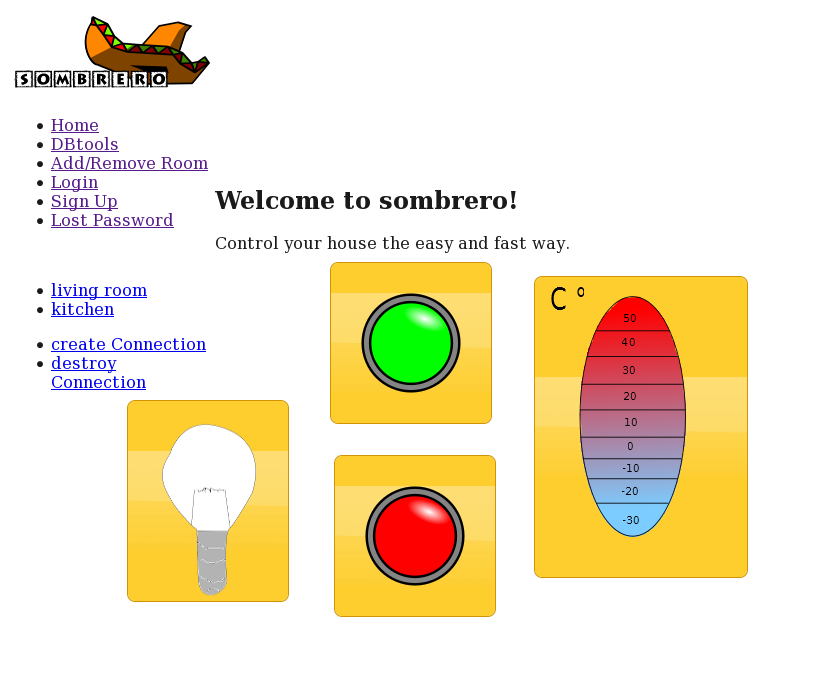
\includegraphics[width=0.80\linewidth]{iteration1.png}
  \caption{the humble beginnings}
  \label{fig:iterations1}
  \end{figure}


\clearpage
\subsection{Iteration 2 - Working}
  With a working prototype to start with, we needed to add all the core functionality which was required for the application to be useful in everyday life.

  The main points were:
  \begin{itemize}
    \item Room management had to be simplified.
    \item User functionality had to be integrated into the site concept.
    \item Widget management was needed.
    \item Image uploading functionality for rooms had to be implemented.
    \item We needed some utility widgets, mainly links between rooms, a toolbox for administrators and a favorite bar for users.
    \item KNX support had to be extended to non-Lamp widgets.
    \item Router discovery for establishing a connection to the KNX network had to be implemented.
    \item We \emph{desperately} needed a more appealing design.
  \end{itemize}

  Building on their experience, Gabriel took care of design and layout, improving the widget concept and expanding KNX support while Alexander managed the database and management functionality and implemented KNX utility features.

  At the end of this iteration, the core functionality was there. The site was still incoherent and parts of the code were a mess, but most of it \emph{worked} and it would have probably been usable by someone brave enough.

  \begin{figure}[h]
  \centering
  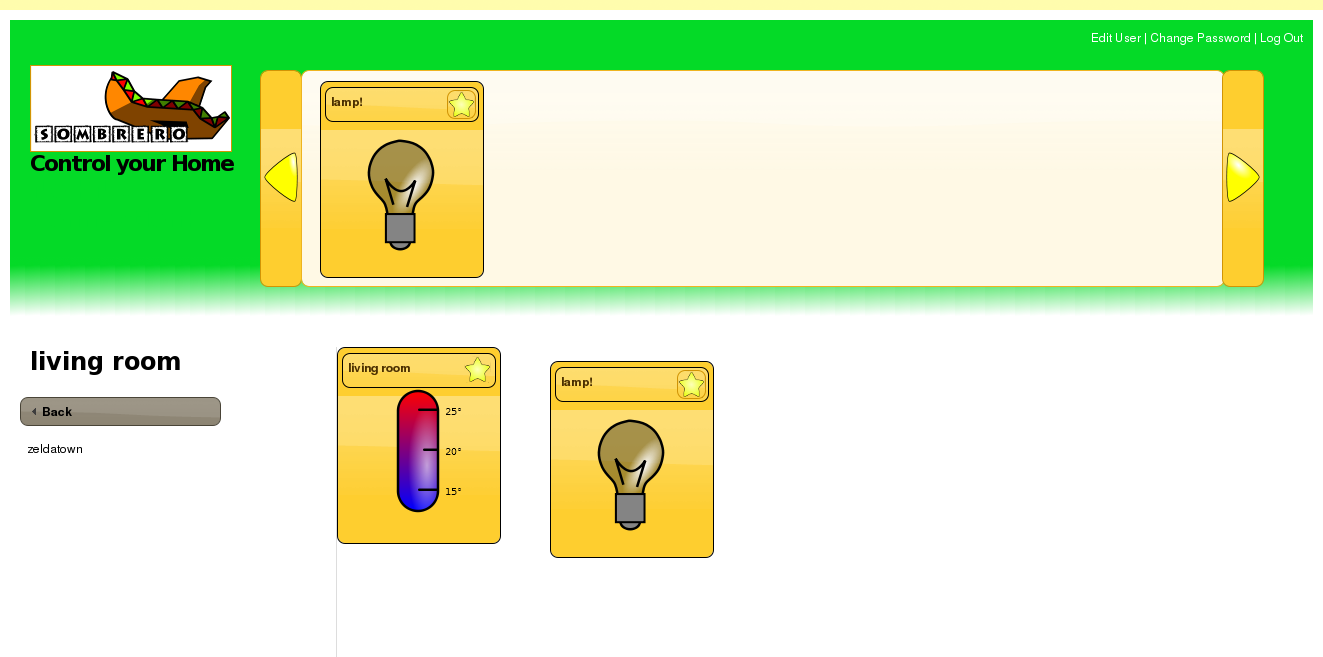
\includegraphics[width=0.80\linewidth]{iteration2.png}
  \caption{shiny new style}
  \label{fig:iterations2}
  \end{figure}

\clearpage
\subsection{Iteration 3 - Finishing}
  As we had little time for the implementation, the third iteration was also the last one. Core functionality was in place, but the whole image was a bit rough around the edges. Widgets still had some bugs and database functionality was mostly hidden behind secret URLs.

  In this iteration we set out to polish the application for shipping and further improve functionality. Unfortunately, Gabriel got sick and we had to drop most of the planned functionality additions. Another goal for this iteration was to clean up the code so it would be easier to read and make additions.

  Gabriel made great improvements to the widgets, fixing lots of bugs and cleaning the code to readability. He also improved widget handling by disallowing them to overlap or leave their predefined space. Another big point of improvement is the separate dialog design he established during this iteration, making dialogs more beautiful and usable.

  Alexander improved user management and widget handling on the server side. He implemented the user list, which allows the administrator to modify other user's accounts. He also wrote a framework which allows widgets to be updated client-side in response to server-side events, which both of us had spent a lot time planning. In adition, Alexander created a grouping system for widgets which was needed for this to work.

  In the end, we managed to get most of our ideas done, creating a complete piece of software. While a bit of further testing couldn't hurt, we believe it is relatively stable, useable and comfortable.

  \begin{figure}[h]
  \centering
  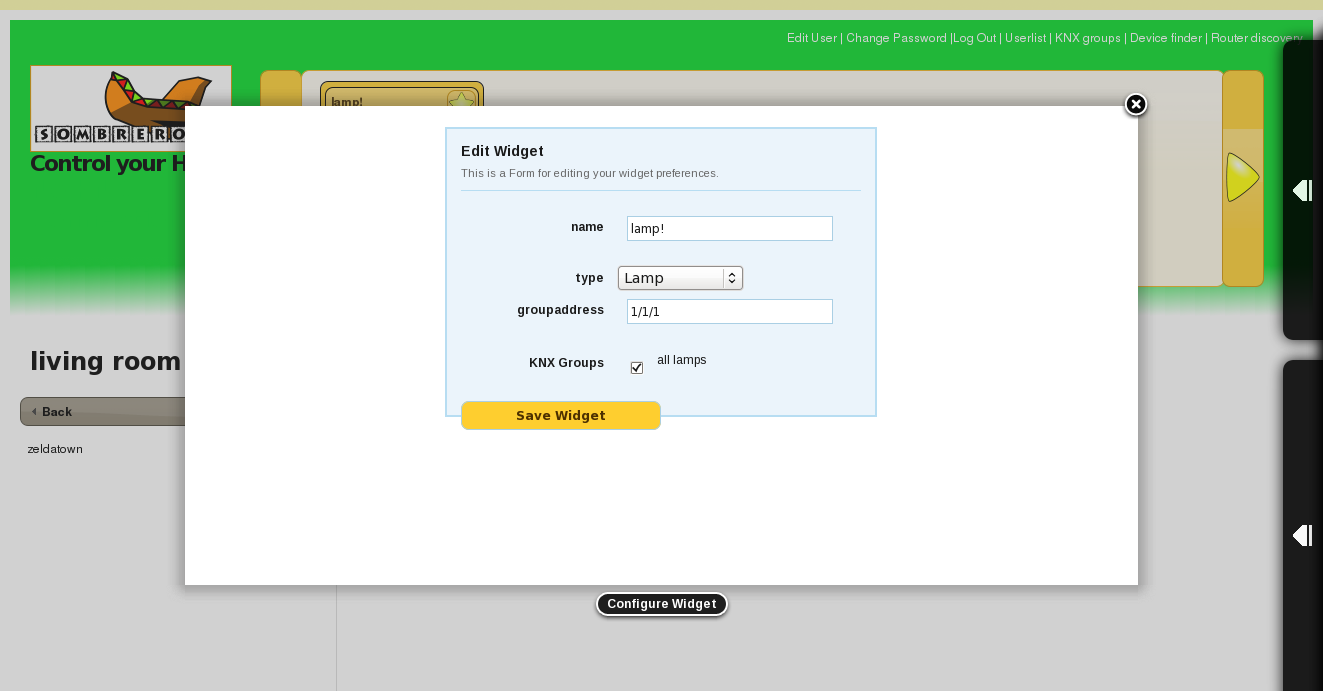
\includegraphics[width=0.80\linewidth]{iteration3f2.png}
  \caption{new dialogs}
  \label{fig:iterations3f1}
  \end{figure}

  \begin{figure}[h]
  \centering
  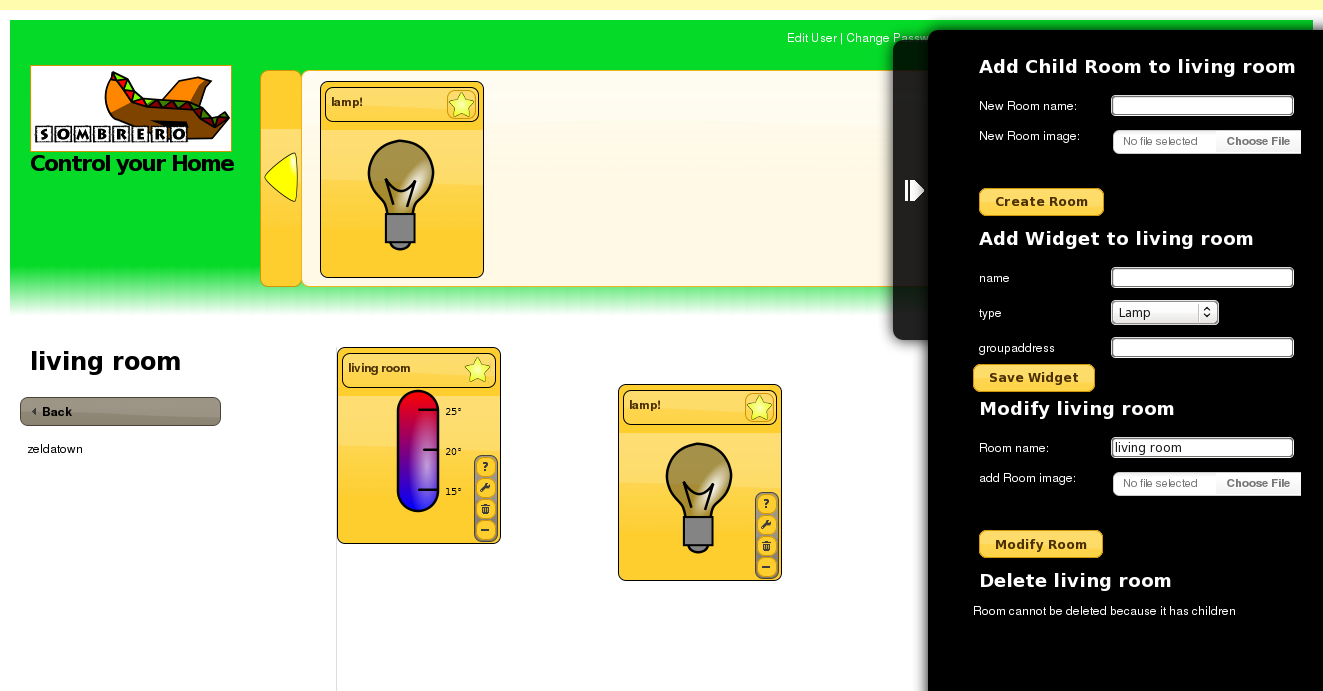
\includegraphics[width=0.80\linewidth]{iteration3f1.png}
  \caption{improved admin mode}
  \label{fig:iterations3f2}
  \end{figure}

\clearpage
%\chapter{Project Progression}
\section{Challenges}
\subsection{New Technologies}
    In sombrero we used many technologies that were completely new to us. That means that we had to learn them from scratch. About two months of our project duration were spent mostly on learning these technologies. Another challenge we encountered was the fact that some parts of Lift weren't properly documented. Lift is a very young framework and hasn't got many committers, so as we decided to use it we knew that we could have problems because of that.
\subsection{Illness}
    The team member Gabriel Grill got ill and wasn't able to do any kind of work for 3 to 4 weeks. That's about the duration of a whole iteration. It happened during the last iteration and because of this illness we weren't able to finish the iteration in time. So during the end of the project we really got into a hurry.
\subsection{Collision Detection between Widgets}
    This challenge has proven itself to be very difficult to solve. After a long search on the internet we found a JQuery plugin that was praised to give Draggable widgets the ability to detect collisions and then position the widgets on the edge of the other one. This algorithm wasn't recursive and didn't check if the dragged widget was inside the bounds of the layout. So it was very bug prone and not really of any use to us. The only solution was to implement it by ourselves, which wasn't as easy as we thought it would be. The drag event doesn't get called for every pixel the dragged widget passes. It depends on how fast you move your widget. So the faster you move the fewer events are called.
\subsection{The perfect project management tool}
    With Getting Real we got a really great guide on how to realize a project successfully, but the toolset to coordinate a project wasn't included in that package. So we had to find ways of our own to coordinate our work. First we tried to manage everything through Google Sites and Google Docs. At the beginning everything went smoothly, but we weren't able to keep everything well structured. Google Sites just wasn't built for project work, but rather for representation. So we switched to GitHub. This went very smoothly, because we also decided to get rid of CVS at the same time. So we used GitHub as code and project management base. After some weeks we discovered that GitHub's support for project management was too weak for our needs. We eventually switched to Pivotaltracker and are still using it today.
\subsection{Testing of Sombrero}
    The testing in sombrero turned out to be very difficult, because it's a web application and that's why we weren't able to think of a lot of unit tests. Whenever we wanted to test the KNX part of the application we had to go to our client to Vienna.
\subsection{CVS vs. Git}
    As a version management tool we decided to use CVS, because there is a ready to use server at our school. After some time of committing and refactoring we became aware of the fact that in CVS it's impossible to delete folders. The only thing you can do is emptying them.

    Another thing that got on our nerves was that when you update your project all version conflicts are just written into their respective files. So eventually we had enough of CVS and switched to another tool. We chose Git, because it's easy to manage and we got rid of all the problems we had with CVS.
\subsection{Eclipse Support}
    Gabriel Grill used eclipse to work on sombrero and encountered different challenges while doing so. The Scala plugin was in beta state, so many features you are used to as a programmer where not fully functional, for instance code completion, debugging and even displaying compiler errors.

    Until the end of the project the Git plugin had no support for merging branches.
\subsection{Challenges Concerning Mapper}
    We used the Lift Mapper as an API for accessing the database. During the development of sombrero we encountered some problems, because of the lack of documentation. A major problem was that a column can not be primary key and a foreign key at the same time. Also the inheritance mechanisms weren't easy to handle, because of the complex type system of Scala.
\clearpage
\section{Project log}
\subsection{Gabriel A. Grill}
\begin{tabular}{| r c r | r | p{9cm} |}
\hline
& & Date & Hours & Description \\
\hline
9/21/2009	&	-	&	9/25/2009	&	5	&	developing project ideas \\
	&		&	9/25/2009	&	1	&	meeting about last year's project \\
9/25/2009	&	-	&	9/30/2009	&	6	&	developing project ideas \\
	&		&	9/30/2009	&	5	&	meeting with client \\
	&		&	10/1/2009	&	2	&	meeting about sombrero \\
	&		&	10/1/2009	&	5	&	writting rudimentary concept for project \\
	&		&	10/2/2009	&	1	&	meeting about sombrero \\
	&		&	10/3/2009	&	2	&	writing changes to description \\
	&		&	10/4/2009	&	1	&	writing changes to description \\
	&		&	10/6/2009	&	2	&	writing changes to description and pitching sombrero \\
	&		&	9/10/2009	&	4	&	looking for modern ways to write sombrero and trying Scala for the first time \\
	&		&	10/15/2009	&	2	&	writing application form \\
	&		&	10/16/2009	&	4	&	redesigning sombrero and deciding on Scala and Lift \\
	&		&	10/19/2009	&	2	&	setting up first package- and class diagram \\
	&		&	10/23/2009	&	5	&	making a first handwritten sketch of the sombrero GUI \\
	&		&	10/24/2009	&	5	&	designing lamp, dimmer and temperature widget and creating rudimentary mock-up \\
	&		&	10/30/2009	&	5	&	working on design, class- and package diagram and writing function spec \\
	&		&	11/5/2009	&	1	&	meeting about functional spec \\
11/6/2009	&	-	&	11/13/2009	&	10	&	working on functional spec and developing a first lift application \\
	&		&	11/19/2009	&	2	&	handing functional spec over and deciding on methodology \\
11/21/2009	&	-	&	11/25/2009	&	2	&	researching on "Agile Programming" and "Getting Real" \\
	&		&	11/25/2009	&	2	&	meeting and presentation of "Getting Real" \\
	&		&	11/26/2009	&	3	&	working on logo and project web site \\
11/28/2009	&	-	&	11/26/2009	&	19	&	working on adoption of "Getting Real" for sombrero and reading it \\
12/20/2009	&	-	&	1/31/2010	&	18	&	working on project web site \\
	&		&	12/21/2009	&	10	&	meeting with client \\
	&		&	12/23/2009	&	3	&	importing sombrero with a first mock-up into CVS \\
1/3/2010	&	-	&	1/7/2010	&	17	&	writing a first rudimentary lamp widget and learning JQuery and setting up JavaScript and CSS framework \\
1/7/2010	&	-	&	1/21/2010	&	17	&	writing a first rudimentary temperature widget \\
1/7/2010	&	-	&	1/21/2010	&	5	&	learning Calimero NG \\
\end{tabular}

\begin{tabular}{| r c r | r | p{9cm} |}
& & Date & Hours & Description \\
\hline
	&		&	1/20/2010	&	6	&	writing Scala classes for the widgets to enable database support \\
	&		&	1/21/2010	&	4	&	completing iteration 1 \\
1/22/2010	&	-	&	1/25/2010	&	5	&	preparing for the end of term presentation \\
2/1/2010	&	-	&	2/4/2010	&	5	&	setting up sombrero wiki \\
	&		&	2/2/2010	&	4	&	refactoring, fixing CVS problems, improving eclipse support and working on design \\
	&		&	2/4/2010	&	2	&	working on utility widgets \\
	&		&	2/5/2010	&	5	&	working on treeview widget \\
	&		&	2/6/2010	&	3	&	fixing CVS problem; working on favorits widget \\
2/8/2010	&	-	&	2/19/2010	&	16	&	working on ideas for Refactoring \\
	&		&	2/12/2010	&	2	&	integrating user-management \\
	&		&	2/20/2010	&	8	&	studying and creating Scala- and Cometactors; setting up git repository; studying lift-process chain and working on dialogs \\
	&		&	2/21/2010	&	8	&	working on Actors; finishing Dialog; working on design \\
	&		&	2/22/2010	&	9	&	improving to Dialog and finishing KNXDaemon concept, finishing design \\
	&		&	2/26/2010	&	2	&	reworking design; and fixing CVS problems \\
	&		&	2/27/2010	&	5	&	finishing TreeViewWidget \\
	&		&	3/1/2010	&	4	&	working on design and admintoolbox \\
	&		&	3/2/2010	&	1	&	meeting about sombrero \\
	&		&	3/7/2010	&	6	&	working on Favorits and TreeView widget; working on Usermenu \\
	&		&	3/8/2010	&	8	&	working on TreeView and refactoring of ui.widgets; finishing UserMenu UI \\
	&		&	3/9/2010	&	6	&	working on Favorites (add, remove, vertical) and Toolbox (refactoring) \\
	&		&	3/11/2010	&	3	&	working on Toolbox and Favorites \\
	&		&	3/12/2010	&	5	&	working on roomlink and toolbox and favorites \\
3/13/2010	&	-	&	16/3/2010	&	13	&	working on collision detection \\
	&		&	3/16/2010	&	7	&	refactoring and work on toolbox and favorites \\
	&		&	4/9/2010	&	2	&	creating github account \\
	&		&	4/10/2010	&	3	&	trying to compile latex files, learning Git, learning latex \\
	&		&	4/11/2010	&	4	&	making Github available via eclipse and pushing first version \\
4/13/2010	&	-	&	4/16/2010	&	96	&	SCALA DAYS 2010 \\
4/16/2010	&	-	&	4/19/2010	&	9	&	refactoring \\
	&		&	4/22/2010	&	6	&	working on forms design, writing popup method, fixing some bugs, learning latex \\
	&		&	4/23/2010	&	8	&	finishing forms design, fixing some bugs, finishing adminsidebar \\
	&		&	4/24/2010	&	1	&	finishing collision detection \\
4/30/2010	&	-	&	5/20/2010	&	15	&	writing documentation \\
4/30/2010	&	-	&	5/20/2010	&	20	&	testing and bugfixing \\
\hline
\end{tabular}
\subsection{Alexander C. Steiner}
\begin{tabular}{| r c r | r | l |}
\hline
& & Date & Hours & Description \\
\hline
9/20/2009	&	-	&	9/30/2009	&	10	&	finding ideas \\
	&		&	9/30/2009	&	6	&	first meating with client \\
10/1/2009	&	-	&	10/6/2009	&	13	&	developing project description \\
	&		&	10/9/2009	&	4	&	researching technologies \\
	&		&	10/15/2009	&	2	&	write application form for last year's project\\
	&		&	10/16/2009	&	2	&	researching and deciding on technologies \\
10/16/2009	&	-	&	10/19/2009	&	4	&	improving concept \\
10/23/2009	&	-	&	10/24/2009	&	10	&	developing GUI concept \\
10/30/2009	&	-	&	11/19/2009	&	17	&	writing functional specification \\
	&		&	11/19/2009	&	1	&	deciding on project management direction \\
11/21/2009	&	-	&	11/22/2009	&	4	&	learning Lift \\
	&		&	11/25/2009	&	2	&	finalizing process model \\
	&		&	11/28/2009	&	2	&	creating the logo \\
	&		&	1/8/2010	&	4	&	setting up the database \\
	&		&	1/18/2010	&	4	&	further study of Lift and URL rewriting \\
	&		&	1/18/2010	&	1	&	creating User table \\
	&		&	1/20/2010	&	7	&	implementing room management functionality \\
	&		&	2/23/2010	&	5	&	improving room management \\
2/25/2010	&	-	&	3/2/2010	&	5	&	imrpoving user system \\
	&		&	2/27/2010	&	2	&	researching image upload \\
	&		&	3/4/2010	&	2	&	creating RoomlinkWidget table \\
	&		&	3/5/2010	&	2	&	implementing container widgets (now dropped)\\
	&		&	3/7/2010	&	2	&	implementing router discovery \\
	&		&	3/7/2010	&	1	&	implementing image display \\
3/9/2010	&	-	&	3/13/2010	&	9	&	implementing widget adding \\
	&		&	3/12/2010	&	2	&	general bugfixing \\
	&		&	3/14/2010	&	5	&	improving widget management \\
	&		&	3/16/2010	&	3	&	implementing KNX listener \\
	&		&	3/16/2010	&	2	&	implementing database support for favorites \\
4/1/2010	&	-	&	4/6/2010	&	4	&	implementing WidgetList\\
	&		&	4/7/2010	&	2	&	general bugfixing \\
4/9/2010	&	-	&	4/10/2010	&	6	&	implementing user management functionality\\
4/10/2010	&	-	&	4/18/2010	&	5	&	developing KNX alias functionality \\
	&		&	4/10/2010	&	2	&	learning LaTeX \\
4/13/2010	&	-	&	4/16/2010	&	96	&	SCALA DAYS 2010 \\
	&		&	4/16/2010	&	3	&	bugfixing and documenting \\
	&		&	4/18/2010	&	2	&	resolving mergind difficulties \\
	&		&	4/18/2010	&	2	&	developing prototype of device finder \\
	&		&	4/22/2010	&	3	&	improving widget editing \\
	&		&	4/22/2010	&	1	&	revising validation rules \\
	&		&	4/24/2010	&	5	&	heavy refactoring of widget forms, fixing lots of bugs\\
	&		&	4/25/2010	&	4	&	finishing device finder and router discovery \\
	&		&	4/25/2010	&	3	&	fixing KNX listener \\
4/30/2010	&	-	&	5/20/2010	&	15	&	writing documentation \\
4/30/2010	&	-	&	5/20/2010	&	20	&	testing and bugfixing \\
\hline
\end{tabular}


\clearpage
\section{Similar Products}

Prior to developing sombrero, we looked at other open source KNX management tools in order to collect ideas and learn from their mistakes. However, we did not find a lot of software that even had KNX support to start with.


\subsection{KNX@home}

KNX@home is a KNX control software similar to sombrero. It is being developed by the University of Applied Sciences in Deggendorf, Germany. The sombrero project originated when Gabriel tried to set up KNX@home during his summer internship. Despite being written in Java and advertised as platform independent, it has lots of dependencies and a very complicated architecture. The only way to get it running was to use the offered live CD. It was then that Gabriel noticed they were only supporting Lamps and had most likely spent most of their time getting their architecture and JavaScript frontend to work. As a consequence, we decided to use a straightforward architecture and powerful frameworks so we could concentrate on more important issues.


\subsection{LinuxMCE}

The goal of LinuxMCE is not to create a KNX control software, but rather a whole smart home framework, including media, telecom, security and building automation. As such, the focus is not on proper KNX support, and setting it up is difficult and requires advanced knowledge of Linux. Also, as the name suggests, LinuxMCE is tied to the Linux platform.

\clearpage
\section{Scala Days 2010}

In May, we noticed that the Scala Days 2010 were coming along, and decided to go there, hoping to learn something that could help us with sombrero. The Scala Days 2010 were the first Scala workshop, and were held at EPFL in Lausanne, Switzerland, on the 15th and 16th of April. While we had a wonderful time and learned a lot, we were not able to use any of the new technologies in sombrero as there was to little time left and the project was already far advanced.

If we do get the opportunity to further improve sombrero, we would most surely make use of the knowledge we earned at Scala Days. The first step would be to rebase to Scala 2.8, which provides exciting new features we would like to use, most importantly package objects, which are packages with member variables and functions, and named and default parameters. Another tool we would like to use is sbt, the Scala build tool. Sbt is fully configurable in Scala and was designed to ease Lift development, so it's a perfect fit for sombrero. We were also very delighted to hear that Eclipse support will improve with the release of Scala 2.8.

\clearpage
	\clearpage
    \chapter{Technology}
%\chapter{Technologies}
\section{KNX}
``More convenience, more safety, higher energy savings: The demand for building management systems is continuously increasing.

Whether in a single-family house or in an office complex, the demand for comfort and versatility in the management of air-conditioning, lighting and access control systems is growing. At the same time, the efficient use of energy is becoming increasingly important. More convenience and safety coupled with lower energy consumption can however only be achieved by intelligent control and monitoring of all products involved. This however implies more wiring, running from the sensors and actuators to the control and monitoring centers. Such a mass of wiring in turn means higher design and installation effort, increased fire risk and soaring costs.

The Answer: KNX /- the Worldwide STANDARD for Home and Building Control''\cite{knx.org}

``KNX is the successor to, and convergence of, three previous standards: the European Home Systems Protocol  (EHS)\footnote[1]{EHS is protocol that's target group were home appliances control and communication using Powerline\footnote[2]{Communication over wires carrying electrical power is called Powerline.}}, BatiBUS\footnote[3]{The BatiBUS is a deprecated field bus.}, and the European Installation Bus (EIB or Instabus)\footnote[4]{EIB describes how sensor and actuators can be connected during installation and how they communicate.}. The KNX standard is administered by the Konnex Association.

KNX defines several physical communication media:

\begin{itemize}
    \item \textbf{Twisted pair wiring (inherited from the BatiBUS and EIB Instabus standards)}
    \item \textbf{Powerline networking (inherited from EIB and EHS - similar to that used by X10\footnote[5]{X10 is a Powerline based home automation protocol.})}
    \item \textbf{Radio (KNX-RF\footnote[6]{KNX Radio Frequency is defined in the KNX specification.})}
    \item \textbf{Infrared}
    \item \textbf{Ethernet (also known as EIBnet/IP or KNXnet/IP)}
\end{itemize}

KNX is designed to be independent of any particular hardware platform. A KNX Device Network can be controlled by anything from an 8-bit microcontroller to a PC, according to the needs of a particular implementation. The most common form of installation is over twisted pair medium.

KNX is approved as an open standard to:

\begin{itemize}
    \item \textbf{International standard (ISO/IEC 14543-3)}
    \item \textbf{Canadian standard (CSA-ISO/IEC 14543-3)}
    \item \textbf{European Standard (CENELEC EN 50090 and CEN EN 13321-1)}
    \item \textbf{China Guo Biao(GB/Z 20965)}
\end{itemize}

KNX has more than 160 members/manufacturers including:

\begin{itemize}
    \item \textbf{ABB}
    \item \textbf{Bosch}
    \item \textbf{Miele \& Cie KG}
    \item \textbf{Schneider Electric Industries S.A.}
    \item \textbf{Siemens}
\end{itemize}

The complete list can be found at \url{http://www.knx.org}.

There are three categories of KNX devices:

\begin{itemize}
    \item \textbf{A-mode or "Automatic mode"}
        devices automatically configure themselves, and are intended to be sold to and installed by the end user.
    \item \textbf{E-mode or "Easy mode"}
        devices require basic training to install. Their behavior is pre-programmed, but they have configuration parameters that need to be tailored to the user's requirements.
    \item \textbf{S-mode or "System mode"}
        devices are used in the creation of bespoke building automation systems. S-mode devices have no default behavior, and must be programmed and installed by specialist technicians.''\cite{wikipedia.org:knx}
\end{itemize}

\clearpage
\section{Calimero}
``Calimero is a Java library for KNX access. It was first presented to the public at the KNX Scientific Conference 2005.
From the beginning, Calimero was also available on SourceForge (versions 1.x). The packages included in this distribution provided a KNXnet/IP (EIBnet/IP) Discovery and Tunneling client, APDU (application layer protocol data unit) type translation services essential for runtime interworking, and a simple group address storage using XML together with a GUI based demo application. Ease of use was a key design goal. Client applications were enabled to communicate with KNX devices via a high level API hiding network protocol details. Since then, development on Calimero continued. When considering new functionality to be included, the question arose how these features could be added while maintaining both ease of use and a compact footprint. Therefore, a considerable reorganization effort was undertaken, leading to a redesign of the user API as well as internal architectural aspects. The new Calimero NG API, in the following only referred to as "Calimero", now supports additional connection protocols, management, property access, high level convenience methods for common tasks, and more.''\cite{auto.tuwien.ac.at:calimeropdf}


In sombrero the ProcessCommunicator class is used to communicate with the KNX devices:
\begin{lstlisting}[caption=Calimero ProcessCommunicator: Connection.scala,label=lst:calimero:connection]
object Connection {
  	var link: KNXNetworkLinkIP = null
	var knxComm: ProcessCommunicator = null

  	def createConnection(remoteHost:String) = {
  		link = new KNXNetworkLinkIP(remoteHost, TPSettings.TP1)
  		if(isConnected){
  			knxComm = new ProcessCommunicatorImpl(link)
  		}
  	}

   def isConnected = link match {
     case null 	=> false
     case x		=> link.isOpen
   }

   def destroyConnection = {
     knxComm.detach
     link.close
   }
}
\end{lstlisting}

The example below shows how messages are sent to and received from KNX devices in sombrero:
\begin{lstlisting}[caption=Calimero write to device: Widget.scala,label=lst:calimero:write]
abstract class KNXWidget[T](destAddress:String, name:String, mainNumber:Int, dptID:String){
	System.out.println(destAddress);
    val destDevice = new GroupAddress(destAddress)
    val dptx: DPTXlator
    val dp: Datapoint

    .
    .
    .

	def write (status: T) = if(Connection.isConnected) Connection.knxComm.write(dp, translate(status))
	def write (status: String) = if(Connection.isConnected) Connection.knxComm.write(dp, status)
}

abstract class StateKNXWidget[T] (destAddress:String, name:String, mainNumber:Int, dptID:String)
		 extends KNXWidget[T](destAddress, name, mainNumber, dptID){
    override val dp = new StateDP(destDevice, name, mainNumber, dptID)

    .
    .
    .

	def getStatus (): Box[T] = {
	  if(Connection.isConnected){
		  Log.info(Connection.knxComm.toString)
		  Full(translate(Connection.knxComm.read(dp)))
	  }else
         Empty
	}
}

abstract class CommandKNXWidget [T] (destAddress:String, name:String, mainNumber:Int, dptID:String)
		 extends KNXWidget[T] (destAddress, name, mainNumber, dptID){
    override val dp = new CommandDP(destDevice, name, mainNumber, dptID)
}
\end{lstlisting}
\clearpage
\section{Scala}

Scala is a general purpose programming language. It is both object-oriented and functional and intends to minimize unnecessary code. It's concise syntax and, as a result, code sizes, can be compared to dynamic languages such as Python, while being statically typed.

As Scala uses the Java Virtual Machine, it is fully interoperable with Java. Scala classes can freely use and even inherit from Java classes and vice versa.

The following chapter is intended as a brief introduction to Scala, with a focus on the techniques used prominently in sombrero's code. It is in no way intended to be a complete guide to Scala. If you would like to learn more about Scala, we recommend looking at its web site, \url{http://www.scala-lang.org/}, and the book 'Programming in Scala' by Martin Odersky, the language's creator.

\subsection{Syntax}

As Scala syntax is fairly different to most other programming languages, here is a short and heavily documented example to illustrate the main differences to Java:

\begin{lstlisting}[caption=Scala Syntax,label=lst:scala:syntax]
//Classes can have parameters. These are equivalent to constructor parameters.
//Types are written AFTER the variable name, separated by a colon.
class Line(p1 : Point, p2 : Point) {

  //Create instance variables.
  //Type is inferred by the compiler.
  //Equivalent to Java: public Point pleft = p1;
  var pleft = p1 //No semicolon needed!
  var pright = p2

  //This code will be run on instanciation.
  //Basically the constructor body.
  //Note that Point.x could be a method since brackets for methods without parameters are not needed
  if(p2.x < p1.x) {
    pleft = p2
    pright = p1
  }

  //A simple function without return value.
  //Equivalent to Java: public void move(int dx, int dy) {
  def move(dx : Int, dy : Int) {
    pleft.x += dx
    pleft.y += dy
    pright.x += dx
    pright.y += dy
  }

  //The '=' denotes a function with return value.
  //Again, types are inferred by the compiler.
  def diff = {
    //The 'val' keyword creates a value (a constant).
    //Immutable values are often used in functional programming style.
    val newx = pright.x - pleft.x
    val newy = pright.y - pleft.y
    //The last statement in a block is the return value.
    new Point(newx, newy)
  }

  //Because operator overloading is supported in Scala, it would be easier to do:
  def diff2 = {
    pright - pleft
    //In fact, this is translated to:
    pright.-(pleft)
  }

  //Shorter syntax without the curly brackets:
  def diff3 = pright - pleft
  def left = pleft.x
  def right = pright.x

  //XML literals
  def toXml=
  <line>
    <point>{pleft.toString}</point>
    <point>{pright.toString}</point>
  </line>
}
\end{lstlisting}


\subsection{Singletons}

Singletons are object values that don't have an enclosing class. They are not fields of an instance, but rather reside inside a package next to classes. Singletons can also be imagined as classes that construct just one instance, but do so automatically. Fields and methods can be accessed through the object name, similar to static references in Java.

A special category of singletons are companion objects. These are simply singletons with the same name as a class. They usually complement the class and are used as a replacement for static methods and fields, which don't exist in Scala. Companion objects are frequently used to create constructors and extractors (the opposite of a constructor). Constructors are usually implemented as the \lstinline!apply! method, which gets called when an object is used as a function (when you put a parameter list next to it).

The following example adds companion objects to existing \lstinline!Line! and \lstinline!Point! classes.

\begin{lstlisting}[caption=Scala Singletons and Companion Objects,label=lst:scala:singletons]
object Line {
  def apply(p1 : Point, p2 : Point) = new Line(p1, p2)
}
object Point {
  def apply(x : Int, y : Int) = new Point(1, 2)
  //apply gets called by doing
  val origin = Point(0,0)
}

//this enables us to create a new Line by:
val line = Line(Point.origin, Point(5,7))
\end{lstlisting}


\subsection{Functions as Values}

In Scala, everything is an object, including functions. That means that you can pass functions or code blocks as arguments to other functions. Where you would use a Runnable in Java, for example, you just pass a function without arguments and return value in Scala.

The next example describes different methods of incrementing all Elements of a list. As lists are by default immutable in Scala, the new list is returned and the old one unmodified. To do this, we use \lstinline!List!'s \lstinline!map! method. It takes a function as a parameter, applies the function to each element of the \lstinline!List! and returns a \lstinline!List! of the return values. To pass a function as a parameter rather than its return value, follow it with an underscore (\lstinline!_!).

\begin{lstlisting}[caption=Scala Function Parameters,label=lst:scala:functions1]
//Define the increment function we want to use later.
def incr(i : Int) = i + 1

//Square brackets indicate type parameters for generics. In Java, you would use angle brackets.
def incrList(l : List[Int]) = l.map(incr _)
\end{lstlisting}

In the next example, we do not define the increment function explicitly. Rather, we make use of inline functions. These can be thought of as function literals, and consist of a parameter list, the character sequence \lstinline!=>! (symbolizing an arrow) and the function body. Scala allows to omitt the dot for method calls, and allows to use curly braces instead of round ones for inline functions so it looks like a code block and libraries can produce syntax indistinguishable from core Scala syntax. The following three lines are functionally exactly the same and just display the possibilities of the Scala syntax.

\begin{lstlisting}[caption=Scala Inline Functions,label=lst:scala:functions2]
def incrList1(l : List[Int]) = l.map((i : Int) => i + 1)
def incrList2(l : List[Int]) = l map ((i : Int) => i + 1)
def incrList3(l : List[Int]) = l map {(i : Int) => i + 1}
\end{lstlisting}

Most of the time, the Scala compiler can infer the types of inline function parameters. Thus, the type definition in the parameter list can be omitted. Because the parameter list no loger holds any essiantial information, it can be dropped as well. The underscore is then used where the parameter would otherwise be. If multiple underscores are used, the mark different parameters. That means that if you need to reference a parameter twice or more, you must name it. Again, the following three lines are equivalent to each other and the examples above.

\begin{lstlisting}[caption=Dropping the Parameter List,label=lst:scala:functions3]
def incrList4(l : List[Int]) = l map {(i) => i + 1}
def incrList5(l : List[Int]) = l map {i => i + 1}
def incrList6(l : List[Int]) = l map {_ + 1}
\end{lstlisting}


\subsection{Pattern Matching}

Pattern matching can be seen as a vastly more powerful alternative to Java's switch/case statements. Instead of just matching values, it can also match types, match and extract an instance's fields, apply wildcards to the fields and apply general tests. Due to its type matching capabilities, it is used as a replacement to the cast operation, although this is not often necessary due to Scala's powerful type system.

\begin{lstlisting}[caption=Scala Pattern Matching,label=lst:scala:patterns]
x match {

  //Match value and type simultaneously.
  case 1 => println("one") //No break needed.

  //Match type.
  case s : String => println(s)

  //Matches are evaluated top to bottom and the first match is executed.
  case i : Int => println("not one: " + i)

  //Match type and apply test.
  case p : Point if p.x > 4 => println("right point: " + p)

  //Extract fields.
  case Point(x, y) => println("left point, x=" + x + " y=" + y)

  //Extract some, match some others, wildcard the rest, and apply a test.
  case Line(Point(x, y), Point(3, _)) if x == y => println("pretty specific line...")

  //Catch everything that was has not yet matched anything.
  case _ => println("something else")
}
\end{lstlisting}


\subsection{Traits}

Traits are similar to Java Interfaces, as they are both used as a substitute to multiple inheritance. In contrast to Interfaces, however, traits can and often do contain implementations for their methods. The process of extending a trait is more commonly refered to as "to mix in the trait". This is often used to add functionality to a class without subclassing it, as the mix in can be applied to subclasses of the class as well while instanciating.

Suppose you would like to always be able to access the median element of your \lstinline!Stack!s and \lstinline!Queue!s. To do this, you make a trait that extends \lstinline!Seq!, \lstinline!Stack!'s and \lstinline!Queue!'s common superclass, and defines the \lstinline!median! method. Then, when instanciating a \lstinline!Queue!, you mix in the new trait and have access to the median method.

\begin{lstlisting}[caption=Scala Pattern Matching,label=lst:scala:patterns]
//_ is used instead of *
import scala.collection.mutable._

trait MedianSeq[A] extends Seq[A] {
  def median = apply(length / 2)
}

val q = new Queue[Int] with MedianSeq[Int]
q enqueue 1; q enqueue 2; q enqueue 3; q enqueue 4; q enqueue 5
q median // 3
q dequeue; q dequeue
q median // 4
\end{lstlisting}


\subsection{Actors}

Scala also implements an actor library similar to Erlang's. The idea behind actors is to avoid race conditions through elimination of shared data. Instead of shared data and parallel access, messages are sent to actors, which are stored in a queue and processed sequentially. When messages are sent, however, type information is lost and has to be regained on the receiving side through pattern matching. Due to pattern matching being used, actors can also react differently to different messages, and any object can be used as a message. Actors are instanciated by using the \lstinline!scala.actors.Actor.actor! method, though sometimes it can become necessary to directly subclass \lstinline!scala.actors.Actor!. Messages are sent to actors using the ! operator. For an example of actor usage, see the lift chapter \ref{NEEDED}.

\clearpage
%\chapter{Technology}
\section{Lift}

The Lift homepage (\url{http://www.liftweb.net/}) states that:
"Lift is an expressive and elegant framework for writing web applications. Lift stresses the importance of security, maintainability, scalability and performance, while allowing for high levels of developer productivity. Lift open source software licensed under an Apache 2.0 license."

It uses Scala as its programming language, which allows for compatibility with Java classes and Java Servlet Containers.

For further reading, we recommend "The Lift Book", \url{http://groups.google.com/group/the-lift-book/}.


\subsection{Templates}

In an effort to truly separate program logic and view, templates were created. Templates can import other templates and call special Scala functions called snippets. Meanwhile, all templates stay XML-conform, allowing them to be edited with most standard HTML and XML editors.

\begin{lstlisting}[caption=Lift Templates: userlist.html,label=lst:lift:templates]
<!-- surrounds the content of this tag with the template file "default-admin" -->
<lift:surround with="default-admin" at="content">

<!-- calls snippet UserList and passes the tag's content -->
<lift:UserList form="POST">
<table>  <tr>
    <td>
      User (click to edit)
    </td>
    <td colspan="3">
      set password
    </td>
    <td>
      delte user
    </td>
  </tr>
  
  <!-- prefixed elements are commonly used with Lift's bind function -->
  <userlist:entries>
  <tr>
    <td>
      <user:link />
    </td>
    <td>
      <user:newPw />
    </td>
    <td>
      <user:newPw />
    </td>
    <td>
      <user:submit />
    </td>
    <td>
      <user:delete />
    </td>
  </tr>
  </userlist:entries>
</table>
</lift:UserList>
</lift:surround>
\end{lstlisting}


\subsection{Snippets}

Snippets are Scala functions designed to be called by templates. They are methods of classes in a designated package, per convention called "snippet". They are then called using \lstinline!<lift:Class.method />!. If no method is given, it defaults to \lstinline!render!. All snippets take a \lstinline!scala.xml.NodeSeq! (the scala class representing XML structures) as a parameter and return a \lstinline!scala.xml.NodeSeq!.

HTML output is most easily generated with the SHtml object, which contains HTML generation methods for most standard uses.

An important method to note here is \lstinline!net.liftweb.util.BindHelpers.bind!, which will most of the time be imported through \lstinline!net.liftweb.util.Helpers!. It takes a prefix name as \lstinline!String!, a \lstinline!NodeSeq! and an arbitrary amount of \lstinline!String!, \lstinline!NodeSeq! tuples, resembling a map from \lstinline!String! to \lstinline!NodeSeq!. It then parses the NodeSeq and replaces any tags of the form \lstinline!<prefix:rest>! with the specified prefix and looks for the rest of the name in the map. Every matching tag is replaced by the map value. This allows designers to place the tags without even knowing what they will be in the end.

Here is the snippet for the template example in the previous section:
\begin{lstlisting}[caption=Lift Snippets: UserList.scala,label=lst:lift:snippets]
class UserList {

  //return type of snippets should be defined manually to avoid compiler confusion
  def render(xhtml : NodeSeq) : NodeSeq = {
    def entry(user : User, insidexhtml : NodeSeq) : NodeSeq = {
      var newPasswd : List[String] = Nil
      
      def testAndSet {
        user.password.setFromAny(newPasswd)
        user.validate match {
          case Nil => user.save; S.notice(user.email.is + "'s password set")
          case xs => S.error(xs)
        }
      }
      
      def testAndDelete {
        if(user.superUser.is && User.count(By(User.superUser, true)) == 1)
          S.error("you can't delete the last admin")
        else
          user.delete_!
      }
    
      //binds <user:something /> tags
      bind("user", insidexhtml,
           //tuple (a, b) can be written as a -> b
           "link" -> link("/useredit/" + user.id.is, () => Empty, Text(user.email.is)),
           "newPw" -> password_*("", LFuncHolder(newPasswd = _)),
           "submit" -> submit("Set Password", testAndSet _),
           "delete" -> submit("Delete User", testAndDelete _)
         )
    }
    
    bind("userlist", xhtml, "entries" -> ((insidexhtml) =>
    User.findAll().flatMap(entry(_, insidexhtml))))
  }
}
\end{lstlisting}


\subsection{Mapper}

Mapper is Lift's Object Relational Mapping (ORM) framework. The idea behind ORM frameworks is to write a class with specific attributes and then store instances of this class in a relational database. In Lift's case, Mapper can take any class extending the \lstinline!net.liftweb.mapper.BaseMapper! trait and create database tables in any database accessible through JDBC. In practice you would use the \lstinline!net.liftweb.mapper.KeyedMapper! or \lstinline!net.liftweb.mapper.LongKeyedMapper! traits because they offer implementations for most of \lstinline!BaseMapper!'s undefined functions.

To construct a Mapper-enabled class, you need a Mapper class and a MetaMapper companion object. The MetaMapper traits include many useful functions for manipulating the database table and fetching objects from the database. Inside the Mapper class, fields to be mapped to the database are defined as objects extending one of the mapped fields, e.g. \lstinline!net.liftweb.mapper.MappedLong! or \lstinline!net.liftweb.mapper.MappedString!.

\begin{lstlisting}[caption=Lift Mapper: Room.scala,label=lst:lift:mapper]
//LongKeyedMapper takes the actual class as a type parameter
//IdPK inserts a long id field that automatically increments
class Room extends LongKeyedMapper[Room] with IdPK {
  //returns the corresponding MetaMapper
  def getSingleton = Room
   
  //creates a string field
  object name extends MappedString(this, 25) {
    //creates a database index for quicker searching
    override def dbIndexed_? = true
  }
   
  object parent extends MappedLongForeignKey(this, Room) {
    override def dbIndexed_? = true
  } 
  
  object image extends MappedBinary(this)
  object imageMime extends MappedString(this,100)
  
  //utility methods
  def widgets = Widget.findAll(By(Widget.room, this.id))
  def children = Room.findAll(By(Room.parent, this.id))
  
  //cascadingly delete associated widgets
  override def delete_! = { Widget.bulkDelete_!! (By(Widget.room, this.id)); super.delete_! }
}  
 
object Room extends Room with LongKeyedMetaMapper[Room] {
  def roots = Room.findAll(By(Room.parent, Empty))
  object currentVar extends RequestVar[Box[Room]](Empty)
  def current = currentVar.is
}
\end{lstlisting}


\subsection{Comet}

Building on Scala's actors, Comet in Lift is implemented through CometActors. A special tag, \lstinline!<lift:comet>!, is also needed. Comet tags need to have a type and a name attribute. Type is the CometActor class wanted, and Name exists to identify multiple different CometActors in a single page. The CometActor can specify a render method like widgets, except that bind's prefix parameter is specified as a global def and the NodeSeq parameter is not needed. This is because the CometActor's tags can be refreshed individually without a page reload and bind is thus implemented as an instance method rather than a singleton method. CometActor also has three receive methods to override, \lstinline!lowPriority!, \lstinline!mediumPriority! and \lstinline!highPriority!. Inside these methods, \lstinline!partialUpdate! and \lstinline!reRender! can be called to send a JavaScript command to the browser and rerender the CometActor (not the whole page!) respectively.

Ajax is often used in conjunction with comet. However, Ajax is extremely easy to use in Lift. Just use one of SHtml's Ajax methods, which asynchronously call Scala functions on the server.

To illustrate the use of CometActors, here is sombrero's implementation of the router discovery:

\begin{lstlisting}[caption=Lift Comet: discovery.html,label=lst:lift:cometxhtml]
<lift:Surround.choose>
    Router IP: <lift:KNXRouter.ip/> <br/>
    
  <!-- comet actor inclusion, name is irrelevant since there is only one comet tag on the page -->
  <lift:comet type="Discovery" name="something">
    <rtr:button/>
    <rtr:entries/>
  </lift:comet>
  
  <lift:KNXRouter.set form="POST">
    <knxrouter:ip/>
    <knxrouter:set/>
  </lift:KNXRouter.set>
</lift:Surround.choose>
\end{lstlisting}

\begin{lstlisting}[caption=Lift Comet: Discovery.scala,label=lst:lift:cometscala]
class Discovery extends CometActor {
  //set binding prefix
  override def defaultPrefix = Full("rtr")
  
  //generate controls
  def render = bind("now" -> Text(model.KNXRouter.get_?.map(_.ip.is) openOr "Nothing!"),
      "entries" -> <table id="routerlist" />,
      "button" ->  ajaxButton("Start discovery", () => {spawn{discover()}; Noop}))
      
  def discover() = {
    //create a new KNX router discoverer and search for routers
    val d = new Discoverer(0, false)
    
    d.startSearch(10, true)
    
    Log.info(d.getSearchResponses.length.toString)
    
    //replace the generated table with a table containing the results
    this ! SetHtml("routerlist",
    <table id="routerlist">
      {d.getSearchResponses.foldLeft(Nil : NodeSeq)
        {(a,b) => a ++
          <tr>
            <td>
              {SHtml.link(".", () =>
                model.KNXRouter.get.
                ip(b.getControlEndpoint.toString).
                save, Text(b.getControlEndpoint.toString))}
            </td>
          </tr>}
      }
    </table>
    )
  }
  
  //forward received JsCmds to the client
  override def lowPriority : PartialFunction[Any, Unit] = {
  case cmd : JsCmd => {
      partialUpdate(cmd)
    }
  }
}
\end{lstlisting}


\clearpage
%\chapter{Technologies}
\section{JavaScript and JQuery}
\subsection{JavaScript}
    JavaScript is a prototype-based\footnote[1]{a style of object-oriented programming in which classes are not present and behavior reuse (inheritance) is performed via a process of cloning existing objects that serve as prototypes} scripting language used mostly in the form of client-side programming to be executed in web browsers. It's also a dynamic language, this means that it executes many common programming commands at runtime. Another feature is the support for first-class functions.

    Despite its name, JavaScript is unrelated to the Java programming language, but nevertheless there are similarities. It was developed by Brendan Eich of Netscape. The name was result of a marketing plot by Netscape and Sun. JavaScript is a trademark of Sun Microsystems.

    Features:
    \begin{itemize}
        \item \textbf{imperative}

            JavaScript supports all the structured programming syntax from C, but since 1.7 it distances it self more and more from C.
        \item \textbf{dynamic}

            Like in most scripting languages, types are associated with values, not variables. Almost everything in JavaScript is an object. With the eval function you can evaluate statements that are represented as a string at run-time.
        \item \textbf{functional}

            JavaScript has support for first class functions, closures and nested functions.
        \item \textbf{other nice features:}

            \begin{itemize}
                \item \textbf{DOM manipulation}

                    JavaScript executed in the web browser can be used to manipulate the DOM of the displayed HTML site.
                \item \textbf{arrays and objects}

                    Another great feature of JavaScript is the support of Arrays and Objects.
            \end{itemize}
    \end{itemize}
\subsection{Ajax}
    ``Ajax (shorthand for asynchronous JavaScript and XML) is a group of interrelated web development techniques used on the client-side to create interactive web applications.''\cite{wikipedia.org:ajax} In sombrero it is used to invoke asynchronously callbacks on the server to update the status of KNX devices or change and save a configuration. If you want more information concerning Ajax look into the The Lift Book\cite{becker:09}.

\subsection{Comet}
``In web development, Comet is a neologism to describe a web application model in which a long-held HTTP request allows a web server to push data to a browser, without the browser explicitly requesting it.''\cite{wikipedia.org:comet} In Lift this is done by a pull mechanism. In sombrero Comet is used to update widgets on the client, for instance if a the name of a widget was changed or the a lamp was turned on. If you want more information concerning Comet look into the Lift Book\cite{becker:09}.

\subsection{JQuery}
    jQuery is a lightweight cross-browser JavaScript library designed to simplify the client-side scripting of HTML. It was released in January 2006 by John Resig and is used by over 27\% of the 10,000 most visited websites.

    ``jQuery is free, open source software, dual-licensed under the MIT License and the GNU General Public License, Version 2.4 jQuery's syntax is designed to make it easier to navigate a document, select DOM elements, create animations, handle events, and develop Ajax applications. jQuery also provides capabilities for developers to create plugins on top of the JavaScript library. Utilising these facilities, developers are able to create abstractions for low-level interaction and animation, advanced effects and high-level, themeable widgets.''\cite{wikipedia.org:jquery}

    The jQuery library is usually a single JavaScript file, containing all its common functions. To include it within a web page use the following mark-up:
    \lstinline!<script type="text/javascript" src="jQuery.js"></ script>!

    JQuery features in more detail:
    \begin{itemize}
        \item \textbf{Chaining}

            Almost every method in JQuery returns a JQuery object, which can be used to call another method. That's why most statements aren't distributed over many lines of code. Another important feature of methods in JQuery is that most of them are implemented using the each method to iterate through a given set, so that the called method is called for every element of the set.
        \item \textbf{Core and Utilities}

            Here is a short list of very important methods of JQuery:

            \begin{itemize}
                \item \textbf{\lstinline!$("CSS3 Selector")!}
                    is also called the JQuery function and takes a string as an argument and returns a set of matched elements.
                \item \textbf{\lstinline!$.each(array, callback)!}
                    iterates through the array and calls for each element of the set the callback with the parameters index and value.
                \item \textbf{\lstinline!$.map(array, callback)!}
                    is similar to the Scala function map. It translates all items in an array or array-like object to another array of items.
                \item \textbf{\lstinline!$.extend(deep, target, object1, objectN)!}
                    merges the contents of two or more objects together into the first object and it's often used as a replacement for inheritance.
            \end{itemize}
        \item \textbf{Attributes}

            Controlling the attributes of DOM elements is quite easy in JQuery:

            \begin{itemize}
                \item \textbf{\lstinline!attr(name)!}
                    get the value of an attribute by name
                \item \textbf{\lstinline!attr(name, val)!}
                    set the value of an attribute by name
                \item \textbf{\lstinline!css(name)!}
                    get the value of a CSS attribute by name
                \item \textbf{\lstinline!css(name, val)!}
                    set the value of a CSS attribute by name
            \end{itemize}
        \item \textbf{Traversing}

            This feature enables JQuery to filter and find nodes in a set.
        \item \textbf{Manipulation}

            The manipulation package gives you the functionality to set or get the content of a set of nodes or even to append and remove nodes from it.
            Here is a short list of some useful methods:

            \begin{itemize}
                \item \textbf{\lstinline!text()!}
                    returns the text inside every node of the matched set
                \item \textbf{\lstinline!text(val)!}
                    changes the text inside every node of the matched set
                \item \textbf{\lstinline!append(val)!}
                    appends val to the last element inside the matched node. If a set of nodes is matched this is done to all of them.
                \item \textbf{\lstinline!clone()!}
                    creates a copy of set of matched nodes.
                \item \textbf{\lstinline!remove()!}
                    removes a set of matched nodes from the DOM.
                \item \textbf{\lstinline!detach()!}
                    removes a set of matched nodes from the DOM. This method those mostly the same as remove, except that it keeps all data associated with the removed elements.
            \end{itemize}

        \item \textbf{Events}

            In JQuery UI mostly all initialization is done on page load, like for instance in sombrero the creation of the widgets and the binding of events. This event is call after the whole page has been fully built up.
            Example:

\begin{lstlisting}[caption=initiazitation of a JQuery UI widget,label=lst:jquery:initwidget]
$(document).ready(function(){
    //widget init
    $(".class").bind('click', function() {
        alert('bar');
    });
    // or shorter with event helpers
    $(".class").click(function(){
        alert('bar');
    });
});
\end{lstlisting}
        \item \textbf{Effects}
            Another great feature of JQuery is the Effects feature. It enables you to animate showing and hiding of DOM elements in a appealing way.
    \end{itemize}

\subsection{JQuery UI}
``JQuery UI provides abstractions for low-level interaction and animation, advanced effects and high-level, themeable widgets, built on top of the jQuery JavaScript Library, that you can use to build highly interactive web applications.

jQuery UI provides a comprehensive set of core interaction plugins, UI widgets and visual effects that use a jQuery-style, event-driven architecture and a focus on web standards, accessibility, flexible styling, and user-friendly design.''\cite{jqueryui.com}

    Some plugins we used:
    \begin{itemize}
        \item \textbf{Draggable}
            gives a set of matched DOM elements the ability to be dragged on the page.
        \item \textbf{Dialog}
            gives a set of matched DOM elements the ability to open a dialog if clicked.
        \item \textbf{Effects}
            enables the programmer to animate the showing and hiding process in an appealing way.
    \end{itemize}

\subsection{JQuery UI CSS framework}
Widgets in sombrero are used to promote harmless div tags to beautiful widgets. So they contain a combination of logic and view and all of them are fully themeable using the JQuery UI CSS framework and plugin specific styles.

``The jQuery UI CSS Framework provide semantic presentation classes to indicate the role of an element within a widget such as a header, content area, or clickable region. These are applied consistently across all widgets so a clickable tab, accordian or button will all have the same "ui-state-default" class applied to indicate that it is clickable. When a user mouses over one of these elements, this class is changed to ui-state-hover, then ui-state-active when selected. This level of class consistency makes it easy to ensure that all elements with a similar role or interaction state will look the same across all widgets.

The CSS Framework styles are encapsulated in a single file called ui.theme.css and this is the file modified by the ThemeRoller application. Framework styles only include attributes that affect the look and feel (primarily color, background images and icons) so these are 'safe' styles that will not affect functionality of individual plugins. This separation means that a developer can create a custom look and feel by modifying the colors and images in theme.css file and know that as future plugins or bug fixes become available, these should work with the theme without modification.''\cite{jqueryui.com}

\subsection{JQuery UI widget factory}
The jquery.ui.widget.js file provides a factory method to create widget classes. Calling the factory creates a widget method used to create and interact with an instance of that widget class. This method can be called from any JQuery DOM node for the initialization or manipulation of the respective widget.

The following default methods are available for each instance, in addition to those provided by the prototype argument:
    \begin{itemize}
        \item \textbf{\lstinline!destroy()!}
            removes the instance from the encapsulated DOM element, which was stored on instance creation
        \item \textbf{\lstinline!option(String key[, String value])!}
            gets or sets an option for this instance
    \end{itemize}

Available properties for each instance:
    \begin{itemize}
        \item \textbf{\lstinline!options!}
            is a mix of defaults with settings provided by the user.
        \item \textbf{\lstinline!element!}
            is a jQuery object always containing the associated DOM element.
    \end{itemize}

Usage:
\begin{lstlisting}[caption=sourcecode of a JQuery UI widget,label=lst:jquery:writewidget]
(function($) {
//This statement assures that in this scope $ = JQuery

$.widget("ui.thewidget", {
   _init: function() {
     // constructor for thewidget
     // "this" is accessible in all methods of the widget
     // except in anoynmous functions
     if (this.options.option) {
       // this.element is a reference to the DOM node associated to
       // to the widget
       this.element.hide();
     }
   },
   _foo: function() {
      // internal functions should be named with a leading underscore
   },
   bar: function(val) {
     // calculate some value and return it
     return 1+val;
   },
   destroy: function() {
       // overrides the default destructor
       $.Widget.prototype.destroy.apply(this, arguments); // call of the super destroy method
        // destroy widget specific stuff
   }
});

$.extend($.ui.thewidget, {
	version: "1.0",
	defaults: {
        option: true   //default value
    }
});

//creates the widget
$("#id").thewidget({
    option: false
});

})(jQuery);
\end{lstlisting}

\clearpage
%\chapter{Technologies}
\section{JQuery Plugins}
\subsection{JQuery-message}
    Version 1.0

    ``This plugin allows you to easily display feedback messages as an unobtrusive overlay. The message fades away automatically after some time, avoiding the need to click an "ok" button or something similar. The user can speed up hiding of the message by moving the mouse or clicking anywhere.''\cite{bassistance.de}

    Usage:
\begin{lstlisting}[caption=JQuery message,label=lst:plugin:message]
$(function() {
    $().message("Hello world!");
    // or
    $("#display").message();
});
\end{lstlisting}

\subsection{JQuery-collide}
    Version 1.0

    Adds collision detection to draggable objects.
    Add "collide: 'block'" when you create a draggable:

\begin{lstlisting}[caption=collison detection,label=lst:plugin:collide]
$(".box").draggable({collide: 'block'});
\end{lstlisting}
    In 'block' mode objects are blocked from overlapping other objects by being snapped to the edge of the object they collided with.

    This library was mostly rewritten, because it didn't support recursive collision detection and it wasn't able to detect a containment.
\subsection{Fancybox}
Version 1.3.0

``FancyBox is a tool for displaying images, HTML content and multi-media in a Mac-style "lightbox" that floats overtop of web page.''\cite{fancybox.net} Mostly all dialogs in Sombrero are created by FancyBox.

\begin{lstlisting}[caption=how to fancybox,label=lst:plugin:fancybox]
    /* uses default settings */
    $("tagname").fancybox();
\end{lstlisting}


\subsection{iPod-style drilldown menu}
    Version  3.0

The iPod-style drilldown menu was created to help users traverse hierarchical data quickly. It's especially helpful when organizing large data structures that don't translate well into traditional tree view menus.

This library was heavily modified by Gabriel Grill. He fixed some bugs, changed some parts of the layout and changed the navigation so it would be possible for users to bookmark the current room. He also managed to change it from a drilldown menu to a side bar menu. For more insight on this topic read the chapter User Mode. 
\clearpage
\section{CSS and Yaml}
\subsection{CSS}
``Cascading Style Sheets (CSS) is a style sheet language used to describe the presentation semantics (that is, the look and formatting) of a document written in a markup language. Its most common application is to style web pages  written in HTML  and XHTML, but the language can also be applied to any kind of XML document, including SVG and XUL.

The CSS specifications are maintained by the World Wide Web Consortium (W3C). Internet media type (MIME type) text/css is registered for use with CSS by RFC 2318 (March 1998).''\cite{wikipedia.org:css}


\subsection{Yaml}
"Yet Another Multicolumn Layout" (short: YAML) is a (X)HTML/CSS framework for creating flexible layouts.

Features:
\begin{itemize}
    \item \textbf{conform to Web standards}
    \item \textbf{flexible layout concept with grids and rows}
    \item \textbf{submittals available}
\end{itemize}

\clearpage
\section{Version Control}

Through all stages of development, version control systems have been used to keep the code up to date across both developer's computers. In the beginning, we used our school's CVS repository, but when we finally had enough of CVS's shortcomings, we switched to a git repository on GitHub.


\subsection{Concurrent Versions System}

CVS is a free and open source revision control system for software projects that dates back to 1986. Due to its age and numerous limitations, it is now mostly replaced by newer systems.

Our main problems with CVS were the following:

\begin{itemize}
  \item CVS's inability to track renaming and movement of files and especially directories was a major hindrance during refactoring.
  \item CVS's conflict management did not fit our tastes.
\end{itemize}


\subsection{Git}

Git's major advantage when compared to CVS is that it was designed as a \emph{distributed} revision control system. That means that every client has a complete clone of the repository and can check out previous versions and other branches without connecting to the server. Moreover, Git assumes that most work is done in branches, so it provides efficient operations for branching and more importantly, merging. Another aspect of Git we liked a lot is that it doesn't create directories that contain no files. In contrast, CVS does not allow you to delete directories, which led to a lot of empty derectories after we changed the package structure while refactoring.

\subsection{Checking out the Sombrero Sources}

To check out the sombrero sources, \lstinline!cd! into an empty directory and \lstinline!git clone git://github.com/grill/sombrero.git!. For further information on the Sombrero sources, see How to Hack Sombrero\ref{NEEDED}.


\clearpage
%\chapter{Technologie}
\section{Development Environment}
\subsection{Eclipse}
    Eclipse is a multi-language software development environment comprising an IDE with a plug-in system.
    
\subsection{Eclipse Plugins}
    In sombrero we used the following eclipse plugins:
    \begin{itemize}
        \item \textbf{Git plugin}


            ``EGit is an Eclipse Team provider for the Git version control system. Git is a distributed SCM, which means every developer has a full copy of the complete history of every revision of the code, making queries against the history very fast and versatile. The EGit project is implementing Eclipse tooling on top of the JGit Java implementation of Git.''\cite{eclipse.org:egit}
        \item \textbf{Scala plugin}


            The Scala plugin is currently beeing developed by Miles Sabin. Its goal is to make the eclipse IDE as comfortable useable for Scala developers as it is for Java developers.
    \end{itemize}
\subsection{Maven}
    Maven is a tool for Java project management and build automation. Maven is offered by the Apache Software Foundation.

    Maven uses the Project Object Model to describe how projects are build. It comes with a set of predefined targets, but they can be changed by changing the pom.xml file.

    Most of maven's functionality is in plugins. A plugin extends the standard maven command mvn with additional commands.

        \lstinline!mvn [plugin-name]:[goal-name]!

    For example to run sombrero you have to run the command:

        \lstinline!mvn jetty:run!

    Another great feature of Maven is the ability to add dependencies to your project. Just write them into your pom.xml file and they are available for your project. These dependencies can even be automatically updated.

    Maven was very useful to our project because plugins are available for CVS and Git. As a result, it was very easy to integrate the Version Management into the build life cycle.

\clearpage
	\clearpage
    \chapter{How to use Sombrero}
\section{Installation}
\subsection{Windows and Linux}
The installation in Windows can be done many ways. The first one would be to download sombrero.war and deploy it into a serverlet container application server, like Tomcat, Jetty or Glassfisch. Another possibility would be to download the root directory of sombrero and to navigate into it. After that the command \lstinline!mvn jetty:run! should be written into the shell and sombrero should run smoothly. By the way this is the only possible solution to run the latest version of sombrero.

Sombrero has been tested with firefox 3.6 and Java 1.6. So if you install these recommended applications there should be no problems concerning sombrero.
\clearpage 
%\chapter{How to Use Sombrero}
\section{User Mode}
\subsection{What is User Mode?}

  If you are logged in as a simple user, you are considered to be in user mode. In user mode you are not able configure the status of devices and the user  profile properties of others. The status of devices can be changed through clicking. An explanation of every widget will follow later on. The profile properties can be set using the edit user form.

  Sombrero was built to make controlling your house very easy, but to use it properly you first have to understand the concept behind it. A house consists of floors. Floors consist of rooms and in rooms there are devices. You can structure your devices your way, each device is represented by a widget contained in a room. This structuring can only be done in admin mode. To access your devices you can use the tree view sidebar positioned on the left side.

  When you are logged in as a user the layout of the sombrero web page is split into 3 parts. On the left you see the tree view sidebar. The favorites bar is positioned on the top of the page. You can use it to quickly access widgets you use often. On the right side of the page there is some space left. This space is reserved for the widgets in their respective rooms.

  \begin{figure}[h]
  \centering
  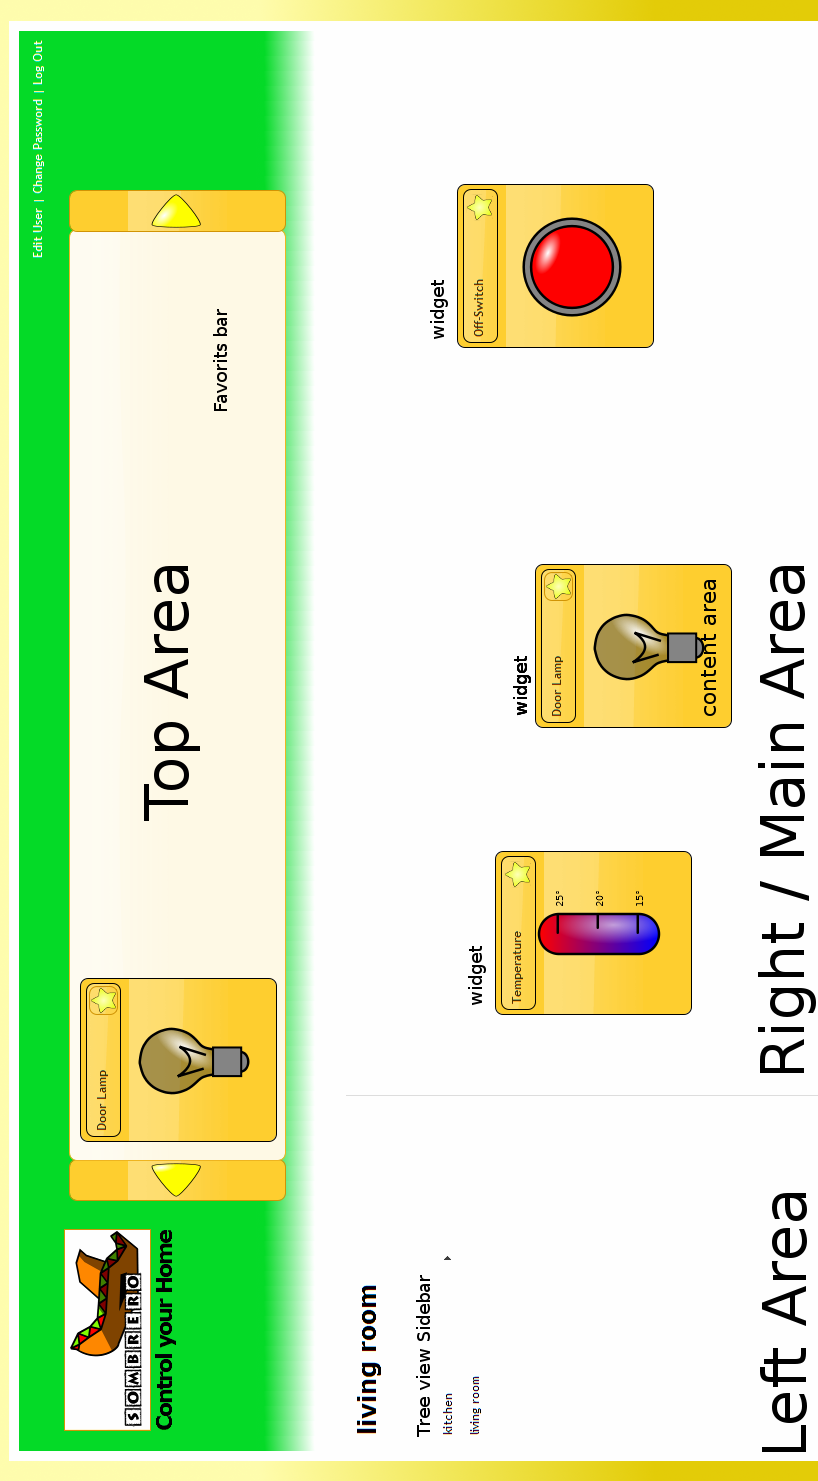
\includegraphics[width=0.80\linewidth]{room3.png}
  %\input{room3}
  \caption{room view structure}
  \label{fig:roomview}
  \end{figure}

  \clearpage
\subsection{Favorites Bar}
  This widget allows you to collect your favorite widgets and quickly access them in every room. The Favorites Bar is also called widget container, because you can add sombrero widgets of almost any kind to it. The content of the Bar stays in the same in every room, so with this widget you can access widgets from another room without being in that room. To add a widget to the Favorites Bar you have to click on the star at the top of the widget. By clicking it again the widget will vanish from the Bar.

\subsection{Tree view Sidebar}
  The tree view sidebar was designed to make navigation between rooms seamless and easy. Just by clicking on the room's name you switch to this room and the tree view sidebar gets updated and displays the rooms in the chosen room. If it has no rooms in it the neighbors are shown. By clicking on the arrow right of the the room name you can switch to the respective room view without loading its content.

  When you navigate into a room which contains rooms, you can go back to the view of the neighbor rooms by clicking the back button on the bottom of the tree view sidebar. Every room has its own URL, so it's possible to bookmark your favorite rooms.

\subsection{Sombrero widgets}
    All widgets that are positioned in the right area of the layout are capable of the following features:
    \begin{itemize}
        \item \textbf{dragging}
            Every Sombrero widget can be dragged in the bounds of the right area of the layout. The position is saved automatically after you drag a widget to a new position.
        \item \textbf{clicking}
            Sombrero widgets are split into two parts. On the top there is the title bar with the name of the widget. Under the title bar there is the content area, containing a selfmade picture of the device the widget represents. By clicking this picture you can change the status or send a command.
        \item \textbf{adding as a favorite}
            The title bar also contains a Star button. By clicking it you add the respective widget to the Favorites Bar and by clicking it again it gets removed. When a widget is up in the Favorites Bar it can also be removed by clicking the Star button of the widget in the Bar. Widgets in the Bar can be used in the same way as if they were down in the right area of the layout.
    \end{itemize}
\subsection{Room Link}
  \begin{figure}[h]
  \centering
  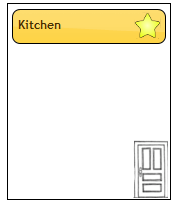
\includegraphics{roomlink.png}
  %\input{roomlink}
  \caption{Room Link}
  \label{fig:roomlink}
  \end{figure}

    This widget is the only one without KNX/EIB functionality. By clicking the picture in the content area of the widget the site will reload and you will find yourself in another room. The Super User has the ability to set a picture for this widget, for example the room the widget links to.
    \clearpage
\subsection{Roller Blind}
  \begin{figure}[h]
  \centering
  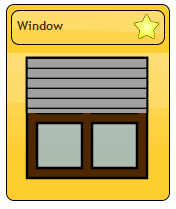
\includegraphics{rollo.png}
  %\input{rollo}
  \caption{Roller Blind}
  \label{fig:rollo}
  \end{figure}

    The Roller Blind is a KNX/EIB device widget. It allows you to control Roller Blinds just by clicking on the Roller Blind. To change state more intuitive, you can move your mouse up and down while it's pressed and the state in which it is in after you released the mouse will be saved.
    \clearpage
\subsection{Temperature actuator}
  \begin{figure}[h]
  \centering
  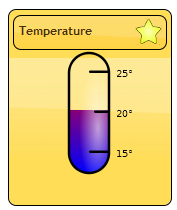
\includegraphics{temperature.png}
  %\input{temperature}
  \caption{Temperature actuator}
  \label{fig:temperature}
  \end{figure}

    This widget is a KNX/EIB device widget and can be used to change temperature of a temperature actuator by clicking the picture in the content area of the widget. To change state more intuitive, you can move your mouse up and down while it's pressed and the state in which it is in after you released the mouse will be saved.
    \clearpage
\subsection{Dimmer}
  \begin{figure}[h]
  \centering
  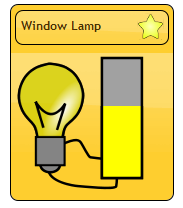
\includegraphics{dimmer.png}
  %\input{dimmer}
  \caption{Dimmer}
  \label{fig:dimmer}
  \end{figure}

    This widget is a KNX/EIB device widget and it is able to change the amount of light emitted from a dimmer by clicking on to the picture in the content area of the widget. To change state more intuitive, you can move your mouse up and down while it's pressed and the state in which it is in after you released the mouse will be saved.
    \clearpage
\subsection{Lamp}
  \begin{figure}[h]
  \centering
  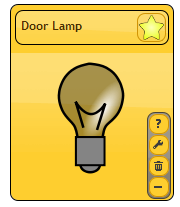
\includegraphics{lamp.png}
  %\input{lamp}
  \caption{Lamp}
  \label{fig:lamp}
  \end{figure}

    The Lamp is a KNX/EIB device widget. It allows you to turn lamps on and off by clicking on to the picture in the content area.
    \clearpage
\subsection{Switch}
  \begin{figure}[h]
  \centering
  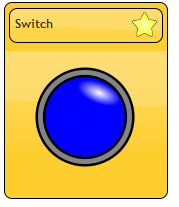
\includegraphics{switch.png}
  %\input{switch}
  \caption{Switch}
  \label{fig:switch}
  \end{figure}

    This widget exists in 3 forms:
    \begin{itemize}
        \item \textbf{Switch}
            With the Switch you can change the state of the device connected to it by clicking on the picture in the content area.
        \item \textbf{Switch Off}
            The Switch Off widget is able to turn the device connected to it off by clicking on the picture in the content area.
        \item \textbf{Switch On}
            The Switch On widget is able to turn the device connected to it on by clicking on the picture in the content area.
    \end{itemize}
\clearpage
%\chapter{How to Use Sombrero}
\section{Admin Mode}
\subsection{What is Admin Mode?}

  If you are logged in as a user with superuser privileges, you are considered to be in admin mode. In admin mode, you are able to do everything a normal user can, but you are shown some additional input elements for managing the room/widget layout and general server setup. Thus, for the purpose of this chapter, it is assumed you are familiar with user mode controls. If there are currently no users with admin privileges, which is most commonly the case after setup if no users have been created yet, all users can be created with admin privileges or take admin privileges through the edit user form. Admin can also give admin privileges to other users through the userlist.

  In admin mode, you can create rooms and widgets through the admin sidebar in room view. Similarly, individual widgets can be modified using the widget configuration buttons while in room view. To configure users and reset passwords, use the user list. To configure the KNX router used to access the KNX network, use the router discovery. To easily add knx widgets, use the device finder. Finally, to set KNX address aliases to match your group address setup, use the KNX group page.

  \clearpage
\subsection{Widget Editing}

  As the widget editing dialog can appear in different places and sometimes different forms, here is a list of widget attributes:
  \begin{itemize}
    \item \textbf{Name:} The name of the widget, which is useful for identifying it among widgets of the same class. It cannot be blank, and while it is possible to give different widgets the same name, it is discouraged to do so.
    \item \textbf{Class:} The class of the widget, or in other words, what this widget represents. Possible values are either different types of KNX widgets (e.g. Lamps or Temperature) and room links. Depending on the class of the widget, the other attributes may change.
    \item \textbf{Attributes of KNX widgets:}
    \begin{itemize}
      \item \textbf{Group Address:} KNX group address of the represented device. If you don't have your devices' group address information at hand, it is perhaps easier to use the device finder.
      \item \textbf{KNX Groups:} Additional KNX group addresses of the device. This is needed to correctly display the device's state.
    \end{itemize}
    \item \textbf{Attributes of Room Links:}
    \begin{itemize}
      \item \textbf{Room Reference:} The room this link leads to when clicked.
      \item \textbf{Image:} The image that is displayed on this room link. It should help to quickly identify the linked room.
    \end{itemize}
  \end{itemize}

\subsection{Admin Sidebar}

  The admin sidebar has two major areas: room modification and the widget clipboard, which can be shown using the upper and lower buttons on the right side of the screen respectively. The room modification area contains forms for adding child rooms to the current room, adding widgets to the current room, directly modifying the current rooms attribute, and deleting the current room.

  You can quickly add widgets too rooms using the widget adding area. Just fill in all the fields, hit "Add Widget", and the widget will appear in the current room. For information on what to enter into the specific fields, see widget editing\ref{NEEDED}.

  The room adding area is used to add rooms to your current layout. Rooms can be used to group widgets and other rooms to mimic their physical layout for easier identification. The room attribute modification area has the same fields, but the changes are applied to the current room instead of a new one. Room rooms can be added in the index page, accessible through the Sombrero logo on the upper left.
  \begin{itemize}
    \item \textbf{Name:} The name of the room. It is the only information the user has of a room when navigating, so choose a meaningful name. It cannot be blank, and while it is possible to give different rooms the same name, it is discouraged to do so.
    \item \textbf{Image:} The background image that is shown when the user visits the room. A good idea is to use a photograph of the room or its floor plan in order to allow users to arrange widgets according to their physical position.
  \end{itemize}

  The widget clipboard is where widgets not currently associated with a room appear. It's handling is similar to the favourites bar. Widgets can be stored here and put back into rooms using the Widget configuration buttons. It should be empty most of the time, as users without admin privileges cannot access the contained widgets.

\subsection{Widget Configuration Buttons}

  While in admin mode, every widget has a configuration bar. It consists of 4 small icons with various functionalities.
  \begin{itemize}
    \item 
\includegraphics{admin-help.png} displays a help page
    \item 
\includegraphics{admin-edit.png} opens the widget editing dialog
    \item 
\includegraphics{admin-delete.png} deletes the widget. Deleted widgets cannot be restored, so be careful.
    \item 
\includegraphics{admin-plus.png} 
\includegraphics{admin-minus.png} removes the widget from the current room and adds it to the clipboard, or vice-versa.
  \end{itemize}

\subsection{User List}

  The user list is the admin's tool to edit other user's accounts. In the column on the left, the user's email addresses are listed. By clicking one of them, you are shown the user editing form known from user mode, but for another user than yourself. By using the password boxes and the "Set Password" button, you can reset user passwords in case someone forgot it. The "Delete User" button deletes the corresponding user. You can even delete other administrators and once deleted, users cannot be recovered, so be careful.

\subsection{Router Discovery}

  This is the page that allows you to view and change the IP address of the KNX router used to access your KNX network. This step is crucial for Sombrero as it is impossible to access any KNX device without it. In most home networks, it will be enough to just hit the "Start Discovery" button and click the first router IP address that pops up. If more than one IP addresses appear, you have more than one KNX router in your network and need to decide which one to use. You can also set the router IP directly via the textbox and the "Set Router IP" button.

\subsection{Device Finder}

  The device finder provides an easy interface for adding KNX widgets when the group addresses are not known (or hard to find). Just press the "Start Device Finder" button and send some KNX commands using other hardware, e.g. switch your light on with the appropriate switch. Addresses which receive 3 or more commands are shown in a list, along with the amount of commands received. Click one of the KNX addresses, and you are presented with a KNX widget adding form. Once the widget is saved, it appears in the clipboard and can be added to the room of your choice.

\subsection{Group Address Aliases}

  KNX group address aliases are needed to correctly identify the device or devices a message is heading to if a device has more than one address. KNX group address alias configuration consists of to two steps.

  First, you have to define the KNX alias addresses. To do this, head to the "KNX Groups". Enter the names and addresses of KNX groups present in your physical setup. Names are just for identification and should be chosen accordingly.

  Second, you have to set the groups your widgets are in. Once you define one or more KNX groups, they appear as checkboxes in the widget editing form. Just check the groups your widget belongs to and save.

\clearpage
	\clearpage
    \chapter{How to hack Sombrero}
\section{Overview}

The most obvious, and thus best supported and easiest change one would probably make to Sombrero is the addition of widgets. Even this task, however, can greatly vary in difficulty and knowledge requirements.

The easiest task is to add KNX support for new devices using our unary, binary or analog widgets. The only thing needed to accomplish this is knowledge of Scala and Calimero, and of course of the KNX device you wish to support. On the represantation side, you just have to supply your own images or reuse ours. It is even easier to specialize our KNX widgets to specific models of devices, as you can use our code as a base.

If you want to add a unique control scheme to your widget, it gets more difficult as you need to script the JQuery representation of your widget and take care of communication between client and server.

To save data other than the KNX addresses, you need to create a new database table. This is basically the same as constructing any Lift Mapper class.

These are the three types of additions discussed in this chapter. If you want to do more than that, for example add your own site, there's no way for us to write a general guide, but it is recommended to take a close look at Lift and JQuery and investigate our templates with similar purpose.

For information on package and class structure, consult Appendix B: Source Structure.

\clearpage
\section{How to create a Widget}
\subsection{Overview}
This capital is a short guide on how to write new widgets. This guide consists of 3 parts:
\begin{itemize}
    \item \textbf{KNX widget - Scala}
        shows you how to implement new KNX widgets just by extending some classes and overwriting some translate methods.
    \item \textbf{KNX widget - JavaScript}
        is a more detailed look on the widget support in sombrero from a JavaScript perspective. This guide should be useful if you need to implement a new UI for a KNX widget.
    \item \textbf{Widgets from scratch}
         will show you how to implement non-KNX based widgets on the example of the room link widget.
\end{itemize}

To understand how widgets in sombrero work you need to understand the widget life cycle.
After a page request has been send to the server, it will be dispatched and the respective page will be generated by Lift. If you load a room view page, sombrero loads all widgets in the respective room from the Database and generates widgets. After that these widgets are rendered into the page, it will be sent to the client. In the next step the browser renders the site and after it's fully loaded all widgets get initialized. Now they are ready for user interaction. If the user performs an interaction which requires server side processing, a callback on the server is invoked via AJAX. There are two possible ways for the server to react and depending on the implementation one is used. The first solution just sends JavaScript commands back, which are later evaluated on the client. The other one is to return nothing to the client and send a request to the distributor actor. The distributer processes the request and sends to all clients affected by the request (using Comet JavaScript) commands to update the UI on the client.

The JavaScript part of the widgets is located in the folder toserve/widgets/js. If a widget needs a great amount of special CSS styles they are outsourced in the folder toserve/widgets/css. All widget Scala files are placed in the package org.sombrero.widget except KNX widgets, which can be found in the org.sombrero.widget.knx package.

\subsection{KNX widget - Scala}
    To bring more structure and modularity to this mess of KNX device widgets we split them into categories. First we differentiate between widgets that have state and ones that are only able to receive commands.

    I think command widgets are rarely used, but can be a nice platform for simple testing of devices. The switch, switch off and switch off are already implemented devices using command widget as a super class.
\begin{lstlisting}[caption=CommandWidget: discovery.html,label=lst:h2h:commandwidget]
abstract class CommandWidget(data: model.Widget, widgetType: String, wp: WidgetPlace) extends Widget(data, widgetType, wp) {

    .
    .

 	/* This method translates a value received from the client into a comprehensible form
     * for the KNX/EIB device encapsulated in this class.
     *
     * @param value is a String received from the client with a range from 0 - 100
     * @returns a String which should be understandable for the devices it will be sent to
 	 */
    def translate(value: String): String
}
\end{lstlisting}

    StateWidget inherits from CommandWidget, because every widget with a state is probably able to change this state. Most KNX widgets have to inherit from this class. Examples of widgets inheriting from this class are lamp, temperature actuator, dimmer and roller blind.
\begin{lstlisting}[caption=StateWidget: Widget.scala,label=lst:h2h:statewidget]
abstract class StateWidget(data: model.Widget, widgetType: String, wp: WidgetPlace) extends CommandWidget(data, widgetType, wp) {

    .
    .

   /* This method translates a value from a KNX/EIB device into an comprehensible form
    * for the clients JavaScript widget encapsulated in this class
    *
    * @param value is a Array[Byte] received from a KNX device
    * @returns a String that will be sent to the client it should hold value between 0 - 100
    */
    def translate(value: Array[Byte]): String
}
\end{lstlisting}

    If you want to implement a new KNX widget, it has to inherit from one of these classes above and implement their abstract methods. When you inherit from one of these classes there are two constructor parameters you need to assign a value to. The one called data can only be assigned by instantiation, because data is an instance of an model.Widget class. That's why it contains all meta data needed to create the widget, like its KNX address or position on site. So it has to be assigned in the constructor of the new class. The other parameter is called widgetType and will be explained in the next paragraph. Another thing you should be careful about is the member variable properties. It contains all properties that will be given as parameters to the JavaScript widget on initialization. All configuration of the UI and JavaScript part of the widgets can be done with this Map. The key is the name of the property and the value is the property's value. To learn more about properties of widget read the chapter JavaScript and JQuery again.

    This form of distinction between KNX device widgets wasn't enough to ensure great modularity, because to keep boilerplate code as small as possible we had to build the same abstraction on the JavaScript level. We discovered that with these two forms of widgets, we wouldn't be able to code the UI and JavaScript part in a modular way. So we decided to create three different widget types. These types are all implemented as standalone widgets and can be configured to become the widgets described in the chapter User Mode.

    Here a list of all available types:
\begin{itemize}
    \item \textbf{unary}
    
        This widget form is equivalent to the command widget. It is possible to configure the picture displayed in the content area. If you click in the content area of the widget a command is sent to the server.

        By inserting this line into the constructor of your new widget the picture in the content area is set to /images/Toogle.png.
\begin{lstlisting}[caption=widget configuration unary: Switch.scala,label=lst:h2h:unaryconfig]
properties ++ Map("img" -> "\"/images/Toggle.png\"")         //img is always displayed
\end{lstlisting}
    \item \textbf{binary}
    
        The binary widgets have two states. It is possible to assign to each state a picture. By clicking in the content area of the widget a command is sent to the server and later a update per Comet is received.

        By inserting this lines into the constructor of your new widget, you can set the pictures displayed in each state.
\begin{lstlisting}[caption=widget configuration binary,label=lst:h2h:binaryconfig]
properties ++ Map(
    "imgOn"  -> "\"/images/lightbulb1.png\"",		             //img displayed if state = true
    "imgOff" -> "\"/images/lightbulb1off.png\""                //img displayed if state = false
)
\end{lstlisting}
    \item \textbf{analog}
    
        This widget form is probably the most common and complex one.
        
        A short introduction to the most important properties:
        \begin{itemize}
            \item \textbf{foreground image}


                This image will always be displayed in foreground.

                \lstinline!frontImg = path!
            \item \textbf{background image}


                This image will always be displayed behind the foreground image.

                \lstinline!backgroundImg = path!
            \item \textbf{which image has to be clipped}


                This property determines which of the two images mentioned above should be clipped. Clipping refers to the CSS property clip, which allows you to cut displayed parts of a selected tag. So this feature gives the widget this feeling of changing the state intuitive. If you want to learn more about this topic read chapter How to use sombrero - User Mode.

                \lstinline!clip_front = true  - the foreground image will be clipped!

                \lstinline!clip_front = false - the background image will be clipped!
            \item \textbf{sliding rectangular}


                By setting this property you determine the area which will be used for sliding to change the state of the widget. All values are relative to the position upper left corner of the content area.

                \lstinline!slideRect = [top, left, height, width]!
            \item \textbf{opacity image}


                This image, if set, will be placed before the foreground widget. It's opacity changes percental to the current state.

                \lstinline!opacity = path!
            \item \textbf{reverse}


                This property allows you to decide if sliding should be top down or bottom up. The lamp and temperature widget are set to top down and the roller blind widget uses bottom up.

                \lstinline!reverse = true  - sliding bottom up!

                \lstinline!reverse = false - sliding top down!
        \end{itemize}

        By inserting one of the following code examples into the constructor of your new widget, you can configure it to look and feel like one of the already finished widgets.
        \begin{itemize}
            \item \textbf{roller blind}
\begin{lstlisting}[caption=widget configuration roller blind: Rollo.scala,label=lst:h2h:rollerblindconfig]
properties ++ Map(
	"frontImg" -> "\"/images/rollo0zu.png\"",
	"backgroundImg" -> "\"/images/rollo0.png\"",
	"slideRect" -> "[19, 19, 122, 122]",
    "reverse" -> "true"
)
\end{lstlisting}
            \item \textbf{temperature actuator}
            \begin{lstlisting}[caption=widget configuration temperature actuator: Temperature.scala,label=lst:h2h:temperatureconfig]
properties ++ Map(
    "clip_front" -> "true"
)
\end{lstlisting}
            \item \textbf{dimmer}
\begin{lstlisting}[caption=widget configuration dimmer: Dimmer.scala,label=lst:h2h:dimmerconfig]
properties ++ Map(
    "frontImg" -> "\"/images/dim0drag.png\"",
	"backgroundImg" -> "\"/images/dim0.png\"",
	"slideRect" -> "[19, 90, 122, 42]",
	"opacity" -> "\"/images/dim0light.png\""
)
\end{lstlisting}
        \end{itemize}
\end{itemize}

To enable KNX support for your new widget, you have to choose the DataPoint of the respective device. There are two categories of KNX devices. One with state and one without. To implement the KNX functionalities you have to write a subclass and implement all abstract methods.

The class CommandKNXWidget should be inherited if you want to use a device without state:
\begin{lstlisting}[caption=KNX command widget: Widget.scala,label=lst:h2h:commandknxwidget]
/* KNXWidget is the super class of the two specified KNX device
 * classes which implement KNX functionality.
 *
 * @type T is a type that should be specified in the last sub
 * class of KNXWidget. This type was built to maintain type
 * conformity.
 */

abstract class KNXWidget[T](destAddress:String, name:String, mainNumber:Int, dptID:String){
	System.out.println(destAddress);
    val destDevice = new GroupAddress(destAddress)
    val dptx: DPTXlator
    val dp: Datapoint

    /* Translate takes a value of type T and transforms it into a
     * String understandable for the KNX device.
     * It was created to maintain type conformity during the
     * sending process of commands.
     */
    def translate (value: T): String

	def write (status: T) = if(Connection.isConnected) Connection.knxComm.write(dp, translate(status))
	def write (status: String) = if(Connection.isConnected) Connection.knxComm.write(dp, status)
}

/* CommandKNXWidget is the super class of all classes which
 * implement Command KNX functionality
 */
abstract class CommandKNXWidget [T] (destAddress:String, name:String, mainNumber:Int, dptID:String)
		 extends KNXWidget[T] (destAddress, name, mainNumber, dptID){
    override val dp = new CommandDP(destDevice, name, mainNumber, dptID)
}
\end{lstlisting}

The class StateKNXWidget should be inherited if you want to use a device with state enabled:
\begin{lstlisting}[caption=KNX state widget: Widget.scala,label=lst:h2h:stateknxwidget]
abstract class StateKNXWidget[T] (destAddress:String, name:String, mainNumber:Int, dptID:String)
		 extends KNXWidget[T](destAddress, name, mainNumber, dptID){
    override val dp = new StateDP(destDevice, name, mainNumber, dptID)

    /* This method takes a value of type String and transforms it
     * into it's respective type.
     * It was written to transform Strings received from a device
     * into it's respective type.
     */
    def translate (value: String): T

    /* This method takes a value of type Array[Byte] and transforms it into a String understandable for humans
     */
    def translate (value: Array[Byte]): String

	def getStatus (): Box[T] = {
	  if(Connection.isConnected){
		  Log.info(Connection.knxComm.toString)
		  Full(translate(Connection.knxComm.read(dp)))
	  }else
         Empty
	}
}
\end{lstlisting}

Here is an example of an already implemented KNX widget with state using binary as a widgetTyp:
\begin{lstlisting}[caption=widget lamp: Lamp.scala,label=lst:h2h:lampwidget]
class Lamp (data: org.sombrero.model.Widget, wp: WidgetPlace) extends StateWidget(data, "binary", wp){
   val knx = new KNXLamp(data.knx().groupAddress.is)
   var status:Boolean = knx.getStatus match {
     case Full(x: Boolean)	=> x
     case _					=> false
   }

   properties ++ Map(
     	"value" -> status.toString
   )
   //sets the path to a helptext URL which can be accessed in Admin Mode
   helpUrl = "/helptext/lamp"

   def translate(value: Array[Byte]): String = knx.translate(knx.translate(value)).toString
   def translate(value: String): String = {
      Log.info("I'm a Lamp tell me what to do");
      knx.translate(! value.toBoolean)
   }
}

class KNXLamp (destAddress:String)
	extends StateKNXWidget [Boolean](destAddress, "Lamp",
			TranslatorTypes.TYPE_BOOLEAN, DPTXlatorBoolean.DPT_SWITCH.getID){
	val dptx = new DPTXlatorBoolean (DPTXlatorBoolean.DPT_SWITCH.getID)

    def translate (value: Boolean): String = {
      dptx.setValue(value)
      dptx.getValue
    }

    def translate (value: String): Boolean = {
      dptx.setValue(value)
      dptx.getValueBoolean
    }

    def translate (value: Array[Byte]): String = {
		dptx.setData(value)
		dptx.getValue
    }
}
\end{lstlisting}

\subsection{KNX widget - JavaScript}
    If you read the previous chapter, you should now be able to implement new KNX widgets with Sombrero's three widget types, but what if want to built a more complex widget? To get some more insight on that part I will show you how we implemented the analog widget. Before reading this chapter you should have read the chapter about how to create JQuery widgets.

    JavaScript sombrero widgets are usually initialized using empty div tags. These tags will be filled with the respective mock-up to make them look and feel like stylish widgets. All the configuration for the widgets is done trough options.

    Because inheritance isn't really supported by JQuery widgets I decided to take another approach to this modularity problem. The solution was to outsource all redundant code into another widget, called protowidget.

    A first look at the \_init method of protowidget:
\begin{lstlisting}[caption=prototype widget - init: ui.protowidget.js ,label=lst:h2h:protowidgetinit]
_init: function (){
	var that = this;                      //this is a helper variable to access this in anonymous functions
	this.hoff = this._getData('hoff');
	this.off = this._getData('off');
	
	this.element
    //these CSS classes give the widget the JQuery UI CSS framework look
	.attr("class", "ui-state-default ui-corner-all")
    //setting all style information that was given by the options
    //this._getData('top') = this.options.top
	.css({
		position: 	"absolute",
		border: 	"1px solid black",
		height: 	(this._getData('height')+this.hoff+this.off) + "px",
		width:		(this._getData('width')+this.off) + "px",
		top: 		this._getData('top') + "px",
		left: 		this._getData('left') + "px"})
    //the hover event
	.hover(function(){ that.mouseOn(); },
			function(){ that.mouseOff(); });   	

	this.toolbox();       //adds the admin toolbox to the widget
	this.draggable();     //adds draggable functionality
	this.titlebar();      //adds the title bar to the widget
}
\end{lstlisting}

    Protowidget consists of the following functionalities:
    \begin{itemize}
        \item \textbf{draggable}

            This feature enables the widgets to be draggable. For this functionality the standard JQuery UI draggable implementation with a small extension is used. The surrounding div tag is used as an associated DOM element.

\begin{lstlisting}[caption=prototype widget - draggable: ui.protowidget.js ,label=lst:h2h:protowidgetdrag]
draggable: function(){
    var that = this;

	this.element.draggable({
		snap: true,
        //enables snapping between widgets
		
        snapMode: "both",
		snapTolerance: "10",
		cancel: this._getData('cancel'),
        //By specifying the property cancel you can
        //state an area that doesn't allow dragging
        //this feature is used by the analog widget
		
        stop: function(event, ui){
        //this function is called when the user stops dragging

				that._setData('top', ui.position.top);
				that._setData('left', ui.position.left);
				that._getData('stop')();
				that._setData('isDragged', true);
		},
		collide: "block",
        //enables collision detection

		containment: this._getData('parentTag')
        //sets a containment tag, which limits
        //widget movement to this area
	});
}
\end{lstlisting}

        \item \textbf{admin toolbox}

            This feature is responsible for the admin toolbox. The protowidget automatically generates the admin toolbox, by specifying the icons that should be used, the callback that should be called and the urls which specify the location for the dialogs. If you want to learn more on this topic feel free to browse through the code.
        \item \textbf{title bar}

            The protowidget also generates the title bar for you. The only thing you need to specify is the title.
        \item \textbf{on hover style change}

            This feature enables the widget to change it's look to a JQuery UI CSS framework hover-look, when the mouse is over the widget.

\begin{lstlisting}[caption=hover widget, label=lst:h2h:hoverwidget]
mouseOn: function(){
	if(!this._getData('hoveroff')) this.element.addClass("ui-state-hover");
},
mouseOff: function(){
	if(!this._getData('hoveroff')) this.element.removeClass("ui-state-hover");
}
\end{lstlisting}

        \item \textbf{copying and moving}

            Copying and moving was developed for the favorites widget and the admin side bar. To enable coping you need to implement the function createCopy. The function should return a copy of the current widget and set is\_active to true and set the parentObj property to the current element.

        Here is an example that shows you how to do so:
\begin{lstlisting}[caption=copy widget, label=lst:h2h:copywidget]
var this = that;

this.element.protowidget( $.extend({}, this.options, {
    createCopy: function(){
		return $('<div></div>').widgetname($.extend({}, that.options, {
			is_active: true,
			parentObj: that.element
		}));
	}
}));
\end{lstlisting}
        \item \textbf{style information}

            By tweaking some options, you can change the style of the widget, for instance height, width or even the position through top and left.
    \end{itemize}
    Every self-built widget that's supposed to be in the main area of the site should use protowidget to enable standard functionality.

Here is an already implemented example:
\begin{lstlisting}[caption=binaray widget: ui.binary.js ,label=lst:h2h:binarywidget]
(function($) {

$.widget("ui.binary", {
	_init: function (){
		var that = this;

		if(this._getData('value'))
			var img = this._getData('imgOn');
		else
			var img = this._getData('imgOff');

		this.element.protowidget( $.extend({}, this.options, {
			createCopy: function(){
				return $('<div></div>').binary($.extend({}, that.options, {
					is_active: true,
					parentObj: that.element
				}));
			}
		}));
		
		this.img = $("<img></img>")
		.css({
			position: 	"absolute",
			height: 	(this._getData('height')) + "px",
			width:		(this._getData('width'))  + "px",
			top: 		this.element.protowidget('option', 'hoff') + "px",
			left: 		"0px"})
		.attr("src", img)
		.click(function (){
			if(!that.element.protowidget('option', 'isDragged'))
				that._getData('change')();
			else
				that.element.protowidget('option', 'isDragged', false);
		})
		.appendTo(this.element);
		
	},
   /* This function should be implemented in every widget with
    * state because it is used as a standard callback by the
    * widget class.
    */
	update_value: function(newValue){
		if(newValue)
			this.img.attr("src", this._getData('imgOn'));
		else
			this.img.attr("src", this._getData('imgOff'));
		this._setData('value', newValue);
	}
});

$.extend($.ui.binary, {
    version: "1.0",     //version number
    defaults: {

top: 0,                 //top value of the widget
left: 0,                //left value of the widget
height: 160,            //height value of the widget
width: 160,	            //width value of the widget
imgOn: "/images/lightbulb1.png",
//img in widget when value = true

imgOff: "/images/lightbulb1off.png",
//img in widget when value = false

click: function(){},    //callback is called on click
stop: function(){},     //callback is called when drag stopped
prefix: "lamp",         //prefix for the id atribute
admin: null,            //true = admin mode - false = normal mode
admin_img: [     "ui-icon-help",
                 "ui-icon-wrench",	
                 "ui-icon-trash",	
                 "ui-icon-minus"],
//array filled with css classes to display
//the clickable icons of the admin widget

admin_onClick: [ function(){},	
                 function(){},		
                 function(){},
                 function(){}],
//callback is called on the click on
//the associated icon of the admin widget

text: "",              //text for the title bar
is_active: false,
//determines if a widget is in the favorites bar or not

favorites: null,
//reference to the JQuery object of the favorites bar

parentTag: null,
//reference to the JQuery object of the main area

active: 	   function(){},
//this callback is called when a widget is promoted to favorite

inactive: 	   function(){},
//this callback is called when a widget looses it's
//favorite status

admin_url: 		[ "",
           		  "" ],
//these strings are urls that are used for creating the help and
//the configuration dialog

in_toolbox:		function(){},
//this callback is called when a widget is moved to the
//admin sidebar

out_toolbox:	function(){},
//this callback is called when a widget is removed from the
//admin sidebar

value: true,		     //true -> on; false -> off

change:			function(){}
//this callback is called when the status of the lamp was
//changed by clicking

	}
});
})(jQuery);

\end{lstlisting}

\subsection{Widgets from scratch}
So far I have shown you how to implement non-KNX widgets and implementing a non KNX widget isn't really different at all.

First you have to create a scala class and let it inherit from org.sombrero.widget.Widget. Then you set the parameter widgetType to the name of the JQuery widget you want to use and as before don't specify data yet. This will be done automatically by the WidgetList class. After that you can add or remove some properties. The next step would be to write the JavaScript part of the widget and after you are done with everything skip to the chapter and read how to write the database part of a widget. After that you should put the widget into the widget list.

This is a modified example of the class WidgetList, where the widget TheWidget was added:
\begin{lstlisting}[caption=widget list ,label=lst:h2h:widgetlist]
object WidgetList {
  case class WidgetClass[T <: model.WidgetData[T]] (name : String, id : String, data : model.WidgetMetaData[T], factory : (model.Widget) => widget.Widget)

  val map = Map(
  "Lamp"        -> WidgetClass[model.KNXWidget]
  ("Lamp", "Lamp", model.KNXWidget, new Lamp(_)),

  "Temperature" -> WidgetClass[model.KNXWidget]
  ("Temperature", "Temperature", model.KNXWidget,
        new Temperature(_)),

  "SwitchOn"    -> WidgetClass[model.KNXWidget]
  ("SwitchOn", "SwitchOn", model.KNXWidget, new SwitchOn(_, _)),

  "SwitchOff"   -> WidgetClass[model.KNXWidget]
  ("SwitchOff", "SwitchOff", model.KNXWidget, new SwitchOff(_, _)),

  "Switch"      -> WidgetClass[model.KNXWidget]
  ("Switch", "Switch", model.KNXWidget, new Switch(_, _)),

  "Dimmer"      -> WidgetClass[model.KNXWidget]
  ("Dimmer", "Dimmer", model.KNXWidget, new Dimmer(_, _)),

  "Rollo"       -> WidgetClass[model.KNXWidget]
  ("Rollo", "Rollo", model.KNXWidget, new Rollo(_, _)),

  "Roomlink"    -> WidgetClass[model.RoomlinkWidget]
  ("Roomlink", "Roomlink", model.RoomlinkWidget, new RoomLink(_, _)),

  "TheWidget"   -> WidgetClass[model.TheWidget]
  ("TheWidget", "TheWidget", model.TheWidget, new TheWidget(_, _)))

 val default = map("Lamp")
}
\end{lstlisting}

If you really want to create a new widget by yourself you should look into the JavaScriptHelper class. There are some quite neat functions for interaction with JQuery widgets and before you start to code your first widget by yourself you should have a look into the file Widget.scala.
\clearpage
\section{Constructing a WidgetData Table}

If you want to save data other than KNX addresses or RoomLinks, you need to build your own \lstinline!WidgetData! table. This consists of a class mixing in \lstinline!WidgetData! and a companion object mixing in \lstinline!WidgetMetaData!, much like you would usually use \lstinline!LongKeyedMapper! and \lstinline!LongKeyedMetaMapper! or similar. \lstinline!WidgetData! handles the foreign key to \lstinline!Widget! and allows for the use of polymorphism in the widget creation and editing forms. \lstinline!WidgetData! does not provide a primary key, so it is recommended to also mix in Lift's \lstinline!IdPK! trait. To get started quickly, just look at the \lstinline!KNXWidget! and \lstinline!RoomlinkWidget! classes. What follows now is a step-by-step example using \lstinline!KNXWidget!.

\subsection{Mix in WidgetData and WidgetMetaData}

For sombrero to correctly recognize your table, you need to mix in \lstinline!WidgetData! and \lstinline!WidgetMetaData! in your class and companion object respectively.

\begin{lstlisting}[caption=Mixing in!,label=lst:widgetdata:mixin]
/*
 * Mix in WidgetData.
 * The type parameter to WidgetData must be the type of the class itself.
 * IdPK is also mixed in to automatically generate a primary key.
 * Note that the primary key must be a Long.
 */
class KNXWidget extends WidgetData[KNXWidget] with IdPK{
  //getSingleton must return the companion object.
  def getSingleton = KNXWidget
}  

/*
 * The companion object must mix in WidgetMetaData.
 * The companion object must also inherit the WidgetData class above,
 * and the type parameter to WidgetMetaData must be that class as well.
 */
object KNXWidget extends KNXWidget with WidgetMetaData[KNXWidget] {}
\end{lstlisting}


\subsection{Create some Fields}

As a table without fields would be pretty useless, we add some to \lstinline!KNXWidget!. In this case, it's a String called groupAddress. Defining fields works the same as in every Mapper class, so consult The Difintive Guide to Lift\cite[chapter 6: The Mapper and Record Frameworks]{becker:09} for further information, they explain it better than I ever could.

\begin{lstlisting}
class KNXWidget extends WidgetData[KNXWidget] with IdPK{
  def getSingleton = KNXWidget
   
  //A basic string field.
  object groupAddress extends MappedString(this, 15) {}
}  

object KNXWidget extends KNXWidget with WidgetMetaData[KNXWidget] {}
\end{lstlisting}


\subsection{Create meaningful Form Generators or Validations}

The create, update and delete operations are automatically available as part of the normal widget configuration methods. WidgetData creation and editing is embedded in the normal widget creation end editing forms through Mapper's \lstinline!toFrom! method and validation framework. In most cases you will need to use at least one of these to guarantee correct user input. This is needed mostly for strings, which usually either validate against a regular expression or provide the user with a drop-down box. To get a drop-down box, override \lstinline!toFrom! and use \lstinline!SHtml.select!, which automatically handles data validation. Again, refer to The Lift Book\cite[as above]{becker:09} for further information. In \lstinline!KNXWidget!'s case, there is no way to get a list of valid group addresses, so we just validate against a KNX address regular expression.

\begin{lstlisting}
class KNXWidget extends WidgetData[KNXWidget] with IdPK{
  def getSingleton = KNXWidget
   
  object groupAddress extends MappedString(this, 15) {
    //Define the validation method as needed by Lift Mapper.
    def correctAddress(in : String) : List[FieldError] = {
      if(Matchers.knx.findPrefixMatchOf(in) == None) {
        List(FieldError(this, Text("incorrect KNX address format")))
      } else {
        List[FieldError]()
      }
    }
    //Generate the List of validations.
    override def validations = correctAddress _ :: Nil
  }
}  

object KNXWidget extends KNXWidget with WidgetMetaData[KNXWidget] {}
\end{lstlisting}


\subsection{Write a Widget}

Now it is time to write the client representation of your widget. This step can actually be done prior or parallel to the previous steps, but needs to be finished before the next one. You can even write more than one widget that makes use of the new \lstinline!WidgetData!.

To access the the instance of your new class that belongs to a widget, use \lstinline!model.Widget.data!. The return type of this function is \lstinline!Box[WidgetData[_]]!, but it always returns a full box with the WidgetData type configured in the \lstinline!WidgetList! (see next step\ref{NEEDED}), unless something already went horribly wrong, so it's no problem if you just die somehow in the default case. As the model widget is located in the widget's data member variable, most accesses to the \lstinline!WidgetData! will look something like this:

\begin{lstlisting}
data.data match {
  case Full(d : MyWidgetData) => d.foo
  case _ => dieHorribleDeath //Should not happen anyways.
}
\end{lstlisting}


\subsection{Insert into WidgetList}

Finally, for sombrero to actually see your new widget and WidgetData, you need to insert it into the \lstinline!WidgetList!. Modifying the widget list works the same as for other custom widgets\ref{NEEDED}, except that you use your new \lstinline!WidgetData! class and companion object instead of \lstinline!KNXWidget! or \lstinline!RoomlinkWidget!. If you did everything right, you should see your new widget class in the selection box in the widget creation form now.

\clearpage
	\clearpage
    \chapter{Ideas for the Future}
%\chapter{Ideas for the Future}
\section{Improvement Suggestions - Sombrero}
In the following chapter I'd like to present some improvement suggestions for sombrero. Most of them are ideas that turned up during project planning or development and were considered for implementation at some point, but have been dropped due to limited resources.

\subsection{Triggers}
This feature was planned for inclusion most of the time, but never really fit into any of the iterations because it requires thorough research of the user interface and serious restructuring on the code side.

The idea is to allow the user to schedule KNX actions that automatically get executed when triggered by some kind of event. Events would mostly be time-based (e.g. turn on the heating at 4 pm so it's warm when you get home from office), but could also originate from KNX measurements (e.g. when the light is turned on, also raise the temperature because it is assumed that some person is inside the room).

To implement this feature, one would have to think of some kind of event system similar to the widgets. Widgets themselves could be used for actions, but a mechanism for accurately specifying the action would be needed (e.g. the exact temperature).


\subsection{Desktop Widgets}
At one point, we had the idea that it would be cool if widgets could be "downloaded" to a user's desktop. Thus, the user would be able to monitor and manipulate selected KNX devices, maybe the lamp in the room the computer is in, without even launching the browser. This wouldn't even be incredibly hard to do, but we just didn't have the manpower to look for a decent desktop widget framework supporting XML, JavaScript and Ajax.


\subsection{Hash Colored Widgets}
While brainstorming on how the user could quickly identify the widgets, the idea to automatically assign a different color to each one came up. The color would be generated out of the name and/or KNX address of the widget, and therefore be unique and never change (as would be the case with random colors). As colors can be quickly identified with a glance, widgets could easily be found. However, because positional information and names can be remembered and identified just as intuitively and random colors are surprisingly hard to do using JQuery, this feature was eventually dropped.


\subsection{Room List}
The room list would allow administrators to manage room and widget layout more easily. Rooms would be laid out in a tree structure similar to the directory index of modern file browsers. Next to the room names, all the widgets in the room would be listed, represented by small icons. When hovering above one of them with the mouse, the full widget would pop up, complete with admin buttons, most notably edit. Widgets and rooms would be moveable and rearrangeable through drag \& drop.

\subsection{Pluggable Widgets}
As of now, it is possible to add custom widgets (See "Hacking Sombrero" \ref{NEEDED}). To do so, however, you have to add your own source files, modify existing ones, and recompile the whole package. It would be ideal if you would just have to drop a file in a specific place and a new widget type would pop up.

\section{Improvement Suggestions - Calimero}
\subsection{Overview}
During our work with sombrero we were lucky to have such an easy abstraction network abstraction library, but as time passed we encountered some difficulties concerning it and its interoperability with Scala. That's why our client suggested that we should add a list of possible improvements for calimero. We put a lot of thought into this and came up with the idea to develop a Scala wrapper library for calimero. The next sections will address some features that would be possible.

\subsection{DSL}
Our first idea was to implement a Domain Specific Language for calimero, to ease and assist learning. This can be done because the Scala language comes with a REPL, a read-evaluation-print-loop. This shell could be used as a platform for beginners to jumpstart calimero learning. It should also be interresting for testing purposes.

\subsection{Generics}
The tuwien.auto.calimero.dptxlator package in calimero contains classes to parse messages recieved from KNX devices into their respective Java types. We would propose to use only one class, that can be dynamicly typed with generics and Scala's implicits. In the current implementation each DPTX type has its own class.

\subsection{Actors}
In calimero all event processing is done by listeners. We had the idea to replace this technology with Actors. The main advantages would be that it's easier to avoid race conditions with actor support and that the whole programm gets more manageable.

\clearpage

	\clearpage
    \chapter{Conclusion}

Building automation, and smart homes in particular, will get increasingly more common and widespread in the next few years. In this diploma thesis project, we tried to develop an easy to use interface to control your intelligent home. While our solution is limited to closed home networks, even this can be used through a smartphone to create a remote control for your entire house. The next logical step would be to test it and make it secure enough to allow access from the internet. Then you would be able to control your house from wherever you are.

To think even further, one could use the various sensors in modern smartphones to detect behaviour patterns and make the house react accordingly. For example, when you are driving home from your skiing holidays, your smartphone will notice this through its GPS sensor and would notify your house, which would then begin heating so its warm and cozy by the time you arrive.

During the creation of sombrero we learned that this and a lot more would already be possible with todays technologies. We hope sombrero will grow to be the technology that provides this functionality.

  \clearpage

  \addcontentsline{toc}{chapter}{Appendix}
  \appendix
  
	%\chapter{Appendix}
\chapter{Curricula Vitae}
\section{Alexander C. Steiner}\begin{tabular}{ll}
\large{Personal Data:}\\ \\
\textbf{E-Mail:}                    &       alex\_steiner@gmx.net\\
\textbf{Date of birth:}             &       08/01/1991\\
\textbf{Citizenship:}               &       Austria\\
\\
\large{Education:}\\
\\
\textbf{2005 - 2010}                &       HTBLuVA Wiener Neustadt \\
                                    &       Department for EDP and Organization\\
\\
\large{Special Skills:}\\
\\
\textbf{Programming Languages:}     &       Scala, Java(ME, SE, EE), C, C\#, Python,\\
                                    &       PHP, JavaScript, Groovy, VBA, SQL, TSQL\\
\textbf{Organization:}              &       RUP, XP, Agile Manifesto, Getting Real\\
\textbf{Frameworks:}                &       Lift, Java, .net\\
\\
\large{Projects:}\\
\\
\textbf{2007-2010}                  &       Robotics Project(RoboCup, Hexapod tournament,\\
                                    &       Robot Challenge)\\
\textbf{2008}                       &       replica file system replication tool\\
\textbf{2008-2009}                  &       TBT(\textbf{T}BT \textbf{B}raille \textbf{T}rainer)\\
\\ \\ \\ \\
\large{Today:}\\
\end{tabular}
\begin{itemize}
\item currently completing his studies at HTBLuVA Wiener Neustadt, EDP and Organization Department
\item world cup finalist of robo cup junior
\item co-author of the KNX management software sombrero
\end{itemize}
\clearpage
\section{Gabriel A. Grill}
\begin{tabular}{ll}
\large{Personal Data:}\\ \\
\textbf{E-Mail:}                    &       gabriel.grill@aon.at\\
\textbf{Date of birth:}             &       02/03/1991\\
\textbf{Citizenship:}               &       Austria\\
\\
\large{Education:}\\
\\
\textbf{2005 - 2010}                &       HTBLuVA Wiener Neustadt\\
                                    &       Department for EDP and Organization\\
\\
\large{Special Skills:}\\
\\
\textbf{Programming Languages:}     &       C, C\#, Java(ME, SE, EE), Groovy, Scala, Matlab, VBA,\\
                                    &       Python, PHP, JavaScript, SQL, TSQL\\
\textbf{Organization:}              &       RUP, XP, Agile Manifesto, Getting Real\\
\textbf{Frameworks:}                &       Lift, Jmaki, JQuery, Java, .net\\
\\
\large{Projects:}\\
\\
\textbf{2007-2010}                  &       Robotics Project(RoboCup, Hexapod tournament,\\
                                    &       Robot Challenge)\\
\textbf{2008-2009}                  &       TBT(\textbf{T}BT \textbf{B}raille \textbf{T}rainer)\\
\textbf{2009}                       &       Smart Library\\
\\ \\ \\ \\
\large{Today:}\\
\end{tabular}

\begin{itemize}
\item currently completing his studies at HTBLuVA Wiener Neustadt, EDP and Organization Department
\item world cup finalist of robo cup junior
\item co-author of the KNX management software sombrero

\end{itemize}

	\clearpage
  \chapter{Source Structure}

\section{Packages}

  \begin{figure}[h]
  \centering
  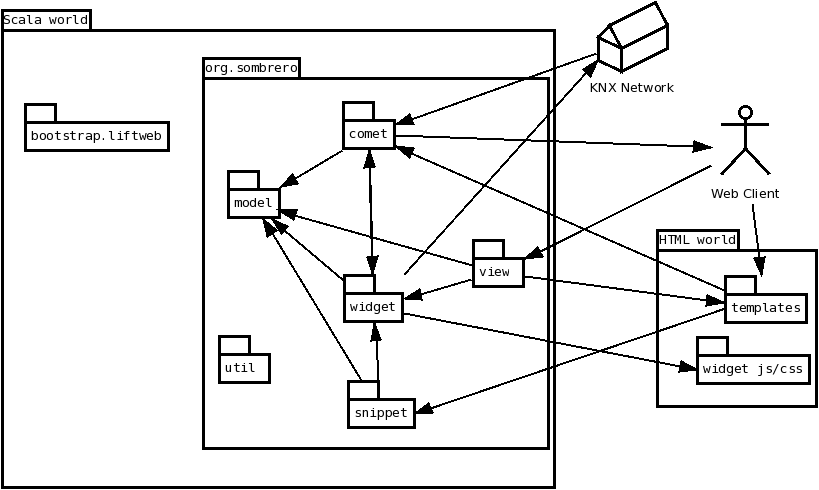
\includegraphics[width=0.80\linewidth]{packages.png}
  %% Graphic for TeX using PGF
% Title: /home/alex/Documents/Schule/Diplomarbeit/diplatex/dia/packages.dia
% Creator: Dia v0.97
% CreationDate: Mon May 17 13:12:52 2010
% For: alex
% \usepackage{tikz}
% The following commands are not supported in PSTricks at present
% We define them conditionally, so when they are implemented,
% this pgf file will use them.
\ifx\du\undefined
  \newlength{\du}
\fi
\setlength{\du}{15\unitlength}
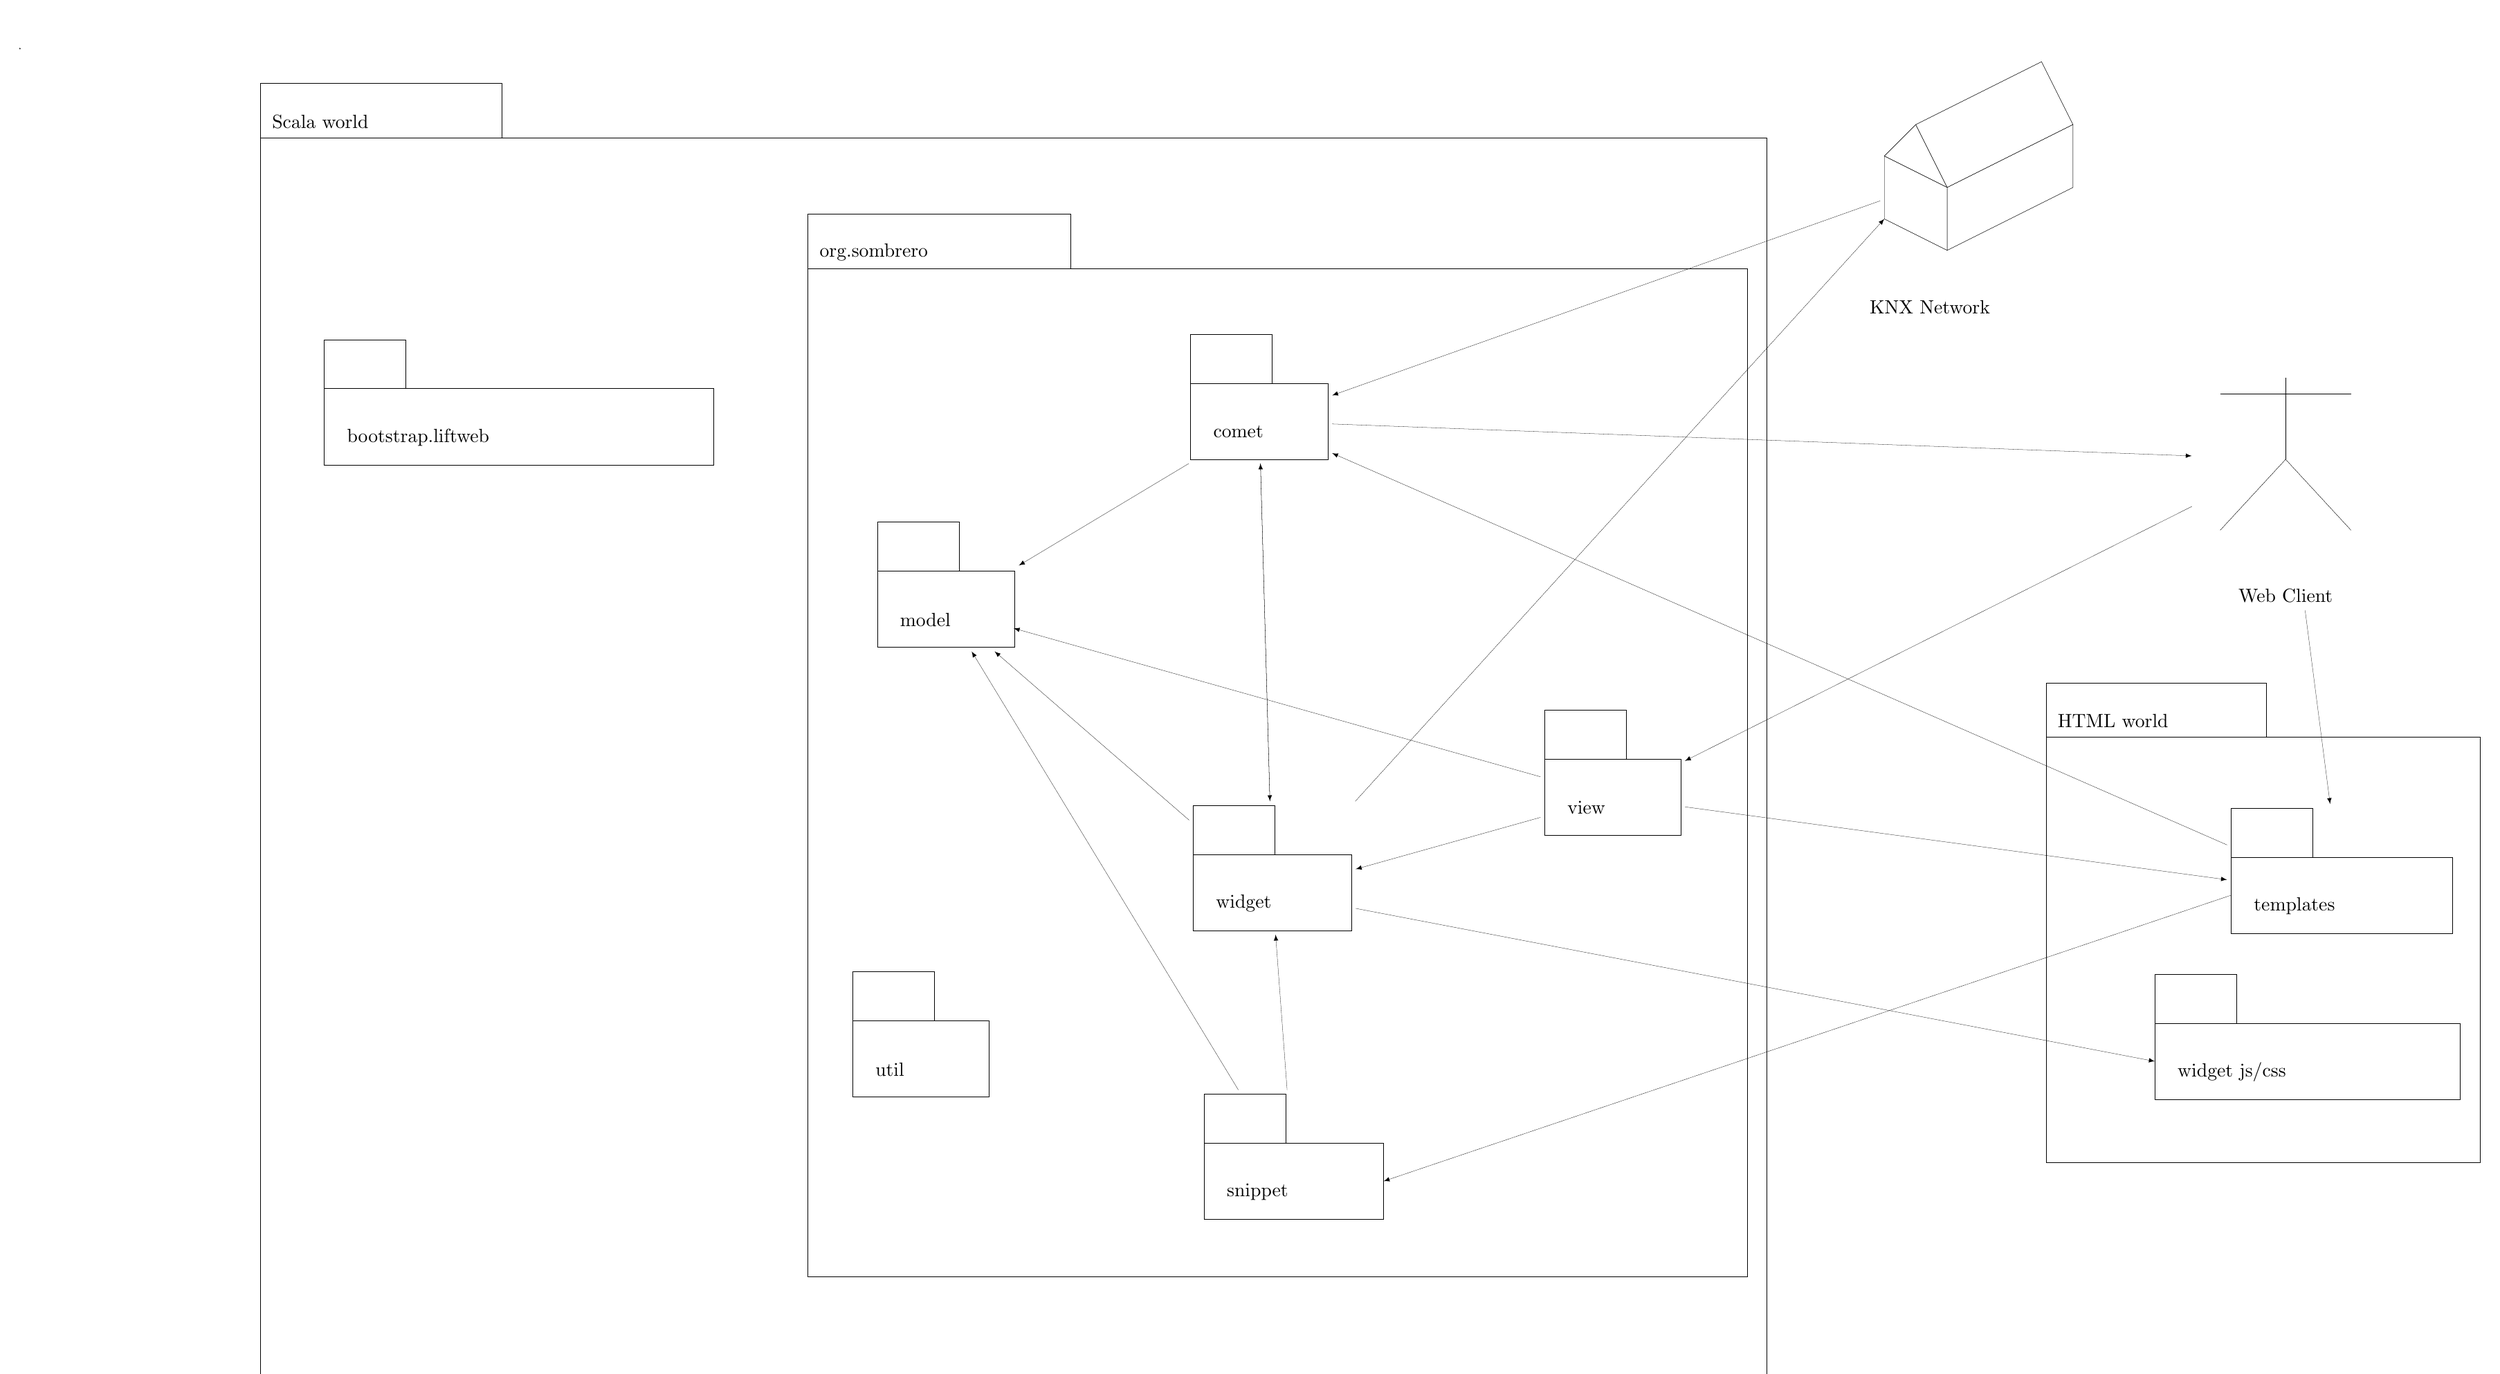
\begin{tikzpicture}
\pgftransformxscale{1.000000}
\pgftransformyscale{-1.000000}
\definecolor{dialinecolor}{rgb}{0.000000, 0.000000, 0.000000}
\pgfsetstrokecolor{dialinecolor}
\definecolor{dialinecolor}{rgb}{1.000000, 1.000000, 1.000000}
\pgfsetfillcolor{dialinecolor}
\pgfsetlinewidth{0.150000\du}
\pgfsetdash{}{0pt}
\definecolor{dialinecolor}{rgb}{1.000000, 1.000000, 1.000000}
\pgfsetfillcolor{dialinecolor}
\fill (38.700000\du,12.850000\du)--(38.700000\du,20.650000\du)--(46.675000\du,20.650000\du)--(46.675000\du,12.850000\du)--cycle;
\definecolor{dialinecolor}{rgb}{0.000000, 0.000000, 0.000000}
\pgfsetstrokecolor{dialinecolor}
\draw (38.700000\du,12.850000\du)--(38.700000\du,20.650000\du)--(46.675000\du,20.650000\du)--(46.675000\du,12.850000\du)--cycle;
\definecolor{dialinecolor}{rgb}{1.000000, 1.000000, 1.000000}
\pgfsetfillcolor{dialinecolor}
\fill (38.700000\du,11.850000\du)--(38.700000\du,12.850000\du)--(42.750000\du,12.850000\du)--(42.750000\du,11.850000\du)--cycle;
\definecolor{dialinecolor}{rgb}{0.000000, 0.000000, 0.000000}
\pgfsetstrokecolor{dialinecolor}
\draw (38.700000\du,11.850000\du)--(38.700000\du,12.850000\du)--(42.750000\du,12.850000\du)--(42.750000\du,11.850000\du)--cycle;
% setfont left to latex
\definecolor{dialinecolor}{rgb}{0.000000, 0.000000, 0.000000}
\pgfsetstrokecolor{dialinecolor}
\node[anchor=west] at (38.800000\du,12.550000\du){HTML world};
\pgfsetlinewidth{0.150000\du}
\pgfsetdash{}{0pt}
\definecolor{dialinecolor}{rgb}{1.000000, 1.000000, 1.000000}
\pgfsetfillcolor{dialinecolor}
\fill (5.925000\du,1.850000\du)--(5.925000\du,24.700000\du)--(33.575000\du,24.700000\du)--(33.575000\du,1.850000\du)--cycle;
\definecolor{dialinecolor}{rgb}{0.000000, 0.000000, 0.000000}
\pgfsetstrokecolor{dialinecolor}
\draw (5.925000\du,1.850000\du)--(5.925000\du,24.700000\du)--(33.575000\du,24.700000\du)--(33.575000\du,1.850000\du)--cycle;
\definecolor{dialinecolor}{rgb}{1.000000, 1.000000, 1.000000}
\pgfsetfillcolor{dialinecolor}
\fill (5.925000\du,0.850000\du)--(5.925000\du,1.850000\du)--(10.360000\du,1.850000\du)--(10.360000\du,0.850000\du)--cycle;
\definecolor{dialinecolor}{rgb}{0.000000, 0.000000, 0.000000}
\pgfsetstrokecolor{dialinecolor}
\draw (5.925000\du,0.850000\du)--(5.925000\du,1.850000\du)--(10.360000\du,1.850000\du)--(10.360000\du,0.850000\du)--cycle;
% setfont left to latex
\definecolor{dialinecolor}{rgb}{0.000000, 0.000000, 0.000000}
\pgfsetstrokecolor{dialinecolor}
\node[anchor=west] at (6.025000\du,1.550000\du){Scala world};
\pgfsetlinewidth{0.150000\du}
\pgfsetdash{}{0pt}
\definecolor{dialinecolor}{rgb}{1.000000, 1.000000, 1.000000}
\pgfsetfillcolor{dialinecolor}
\fill (15.975000\du,4.250000\du)--(15.975000\du,22.750000\du)--(33.225000\du,22.750000\du)--(33.225000\du,4.250000\du)--cycle;
\definecolor{dialinecolor}{rgb}{0.000000, 0.000000, 0.000000}
\pgfsetstrokecolor{dialinecolor}
\draw (15.975000\du,4.250000\du)--(15.975000\du,22.750000\du)--(33.225000\du,22.750000\du)--(33.225000\du,4.250000\du)--cycle;
\definecolor{dialinecolor}{rgb}{1.000000, 1.000000, 1.000000}
\pgfsetfillcolor{dialinecolor}
\fill (15.975000\du,3.250000\du)--(15.975000\du,4.250000\du)--(20.795000\du,4.250000\du)--(20.795000\du,3.250000\du)--cycle;
\definecolor{dialinecolor}{rgb}{0.000000, 0.000000, 0.000000}
\pgfsetstrokecolor{dialinecolor}
\draw (15.975000\du,3.250000\du)--(15.975000\du,4.250000\du)--(20.795000\du,4.250000\du)--(20.795000\du,3.250000\du)--cycle;
% setfont left to latex
\definecolor{dialinecolor}{rgb}{0.000000, 0.000000, 0.000000}
\pgfsetstrokecolor{dialinecolor}
\node[anchor=west] at (16.075000\du,3.950000\du){org.sombrero};
\pgfsetlinewidth{0.150000\du}
\pgfsetdash{}{0pt}
\definecolor{dialinecolor}{rgb}{1.000000, 1.000000, 1.000000}
\pgfsetfillcolor{dialinecolor}
\fill (7.100000\du,6.450000\du)--(7.100000\du,7.850000\du)--(14.245000\du,7.850000\du)--(14.245000\du,6.450000\du)--cycle;
\definecolor{dialinecolor}{rgb}{0.000000, 0.000000, 0.000000}
\pgfsetstrokecolor{dialinecolor}
\draw (7.100000\du,6.450000\du)--(7.100000\du,7.850000\du)--(14.245000\du,7.850000\du)--(14.245000\du,6.450000\du)--cycle;
\definecolor{dialinecolor}{rgb}{1.000000, 1.000000, 1.000000}
\pgfsetfillcolor{dialinecolor}
\fill (7.100000\du,5.550000\du)--(7.100000\du,6.450000\du)--(8.600000\du,6.450000\du)--(8.600000\du,5.550000\du)--cycle;
\definecolor{dialinecolor}{rgb}{0.000000, 0.000000, 0.000000}
\pgfsetstrokecolor{dialinecolor}
\draw (7.100000\du,5.550000\du)--(7.100000\du,6.450000\du)--(8.600000\du,6.450000\du)--(8.600000\du,5.550000\du)--cycle;
% setfont left to latex
\definecolor{dialinecolor}{rgb}{0.000000, 0.000000, 0.000000}
\pgfsetstrokecolor{dialinecolor}
\node[anchor=west] at (7.400000\du,7.345000\du){bootstrap.liftweb};
\pgfsetlinewidth{0.150000\du}
\pgfsetdash{}{0pt}
\definecolor{dialinecolor}{rgb}{1.000000, 1.000000, 1.000000}
\pgfsetfillcolor{dialinecolor}
\fill (17.250000\du,9.800000\du)--(17.250000\du,11.200000\du)--(19.775000\du,11.200000\du)--(19.775000\du,9.800000\du)--cycle;
\definecolor{dialinecolor}{rgb}{0.000000, 0.000000, 0.000000}
\pgfsetstrokecolor{dialinecolor}
\draw (17.250000\du,9.800000\du)--(17.250000\du,11.200000\du)--(19.775000\du,11.200000\du)--(19.775000\du,9.800000\du)--cycle;
\definecolor{dialinecolor}{rgb}{1.000000, 1.000000, 1.000000}
\pgfsetfillcolor{dialinecolor}
\fill (17.250000\du,8.900000\du)--(17.250000\du,9.800000\du)--(18.750000\du,9.800000\du)--(18.750000\du,8.900000\du)--cycle;
\definecolor{dialinecolor}{rgb}{0.000000, 0.000000, 0.000000}
\pgfsetstrokecolor{dialinecolor}
\draw (17.250000\du,8.900000\du)--(17.250000\du,9.800000\du)--(18.750000\du,9.800000\du)--(18.750000\du,8.900000\du)--cycle;
% setfont left to latex
\definecolor{dialinecolor}{rgb}{0.000000, 0.000000, 0.000000}
\pgfsetstrokecolor{dialinecolor}
\node[anchor=west] at (17.550000\du,10.695000\du){model};
\pgfsetlinewidth{0.150000\du}
\pgfsetdash{}{0pt}
\definecolor{dialinecolor}{rgb}{1.000000, 1.000000, 1.000000}
\pgfsetfillcolor{dialinecolor}
\fill (23.000000\du,6.350000\du)--(23.000000\du,7.750000\du)--(25.525000\du,7.750000\du)--(25.525000\du,6.350000\du)--cycle;
\definecolor{dialinecolor}{rgb}{0.000000, 0.000000, 0.000000}
\pgfsetstrokecolor{dialinecolor}
\draw (23.000000\du,6.350000\du)--(23.000000\du,7.750000\du)--(25.525000\du,7.750000\du)--(25.525000\du,6.350000\du)--cycle;
\definecolor{dialinecolor}{rgb}{1.000000, 1.000000, 1.000000}
\pgfsetfillcolor{dialinecolor}
\fill (23.000000\du,5.450000\du)--(23.000000\du,6.350000\du)--(24.500000\du,6.350000\du)--(24.500000\du,5.450000\du)--cycle;
\definecolor{dialinecolor}{rgb}{0.000000, 0.000000, 0.000000}
\pgfsetstrokecolor{dialinecolor}
\draw (23.000000\du,5.450000\du)--(23.000000\du,6.350000\du)--(24.500000\du,6.350000\du)--(24.500000\du,5.450000\du)--cycle;
% setfont left to latex
\definecolor{dialinecolor}{rgb}{0.000000, 0.000000, 0.000000}
\pgfsetstrokecolor{dialinecolor}
\node[anchor=west] at (23.300000\du,7.245000\du){comet};
\pgfsetlinewidth{0.150000\du}
\pgfsetdash{}{0pt}
\definecolor{dialinecolor}{rgb}{1.000000, 1.000000, 1.000000}
\pgfsetfillcolor{dialinecolor}
\fill (23.050000\du,15.000000\du)--(23.050000\du,16.400000\du)--(25.960000\du,16.400000\du)--(25.960000\du,15.000000\du)--cycle;
\definecolor{dialinecolor}{rgb}{0.000000, 0.000000, 0.000000}
\pgfsetstrokecolor{dialinecolor}
\draw (23.050000\du,15.000000\du)--(23.050000\du,16.400000\du)--(25.960000\du,16.400000\du)--(25.960000\du,15.000000\du)--cycle;
\definecolor{dialinecolor}{rgb}{1.000000, 1.000000, 1.000000}
\pgfsetfillcolor{dialinecolor}
\fill (23.050000\du,14.100000\du)--(23.050000\du,15.000000\du)--(24.550000\du,15.000000\du)--(24.550000\du,14.100000\du)--cycle;
\definecolor{dialinecolor}{rgb}{0.000000, 0.000000, 0.000000}
\pgfsetstrokecolor{dialinecolor}
\draw (23.050000\du,14.100000\du)--(23.050000\du,15.000000\du)--(24.550000\du,15.000000\du)--(24.550000\du,14.100000\du)--cycle;
% setfont left to latex
\definecolor{dialinecolor}{rgb}{0.000000, 0.000000, 0.000000}
\pgfsetstrokecolor{dialinecolor}
\node[anchor=west] at (23.350000\du,15.895000\du){widget};
\pgfsetlinewidth{0.150000\du}
\pgfsetdash{}{0pt}
\definecolor{dialinecolor}{rgb}{1.000000, 1.000000, 1.000000}
\pgfsetfillcolor{dialinecolor}
\fill (23.250000\du,20.300000\du)--(23.250000\du,21.700000\du)--(26.545000\du,21.700000\du)--(26.545000\du,20.300000\du)--cycle;
\definecolor{dialinecolor}{rgb}{0.000000, 0.000000, 0.000000}
\pgfsetstrokecolor{dialinecolor}
\draw (23.250000\du,20.300000\du)--(23.250000\du,21.700000\du)--(26.545000\du,21.700000\du)--(26.545000\du,20.300000\du)--cycle;
\definecolor{dialinecolor}{rgb}{1.000000, 1.000000, 1.000000}
\pgfsetfillcolor{dialinecolor}
\fill (23.250000\du,19.400000\du)--(23.250000\du,20.300000\du)--(24.750000\du,20.300000\du)--(24.750000\du,19.400000\du)--cycle;
\definecolor{dialinecolor}{rgb}{0.000000, 0.000000, 0.000000}
\pgfsetstrokecolor{dialinecolor}
\draw (23.250000\du,19.400000\du)--(23.250000\du,20.300000\du)--(24.750000\du,20.300000\du)--(24.750000\du,19.400000\du)--cycle;
% setfont left to latex
\definecolor{dialinecolor}{rgb}{0.000000, 0.000000, 0.000000}
\pgfsetstrokecolor{dialinecolor}
\node[anchor=west] at (23.550000\du,21.195000\du){snippet};
\pgfsetlinewidth{0.150000\du}
\pgfsetdash{}{0pt}
\definecolor{dialinecolor}{rgb}{1.000000, 1.000000, 1.000000}
\pgfsetfillcolor{dialinecolor}
\fill (16.800000\du,18.050000\du)--(16.800000\du,19.450000\du)--(19.300000\du,19.450000\du)--(19.300000\du,18.050000\du)--cycle;
\definecolor{dialinecolor}{rgb}{0.000000, 0.000000, 0.000000}
\pgfsetstrokecolor{dialinecolor}
\draw (16.800000\du,18.050000\du)--(16.800000\du,19.450000\du)--(19.300000\du,19.450000\du)--(19.300000\du,18.050000\du)--cycle;
\definecolor{dialinecolor}{rgb}{1.000000, 1.000000, 1.000000}
\pgfsetfillcolor{dialinecolor}
\fill (16.800000\du,17.150000\du)--(16.800000\du,18.050000\du)--(18.300000\du,18.050000\du)--(18.300000\du,17.150000\du)--cycle;
\definecolor{dialinecolor}{rgb}{0.000000, 0.000000, 0.000000}
\pgfsetstrokecolor{dialinecolor}
\draw (16.800000\du,17.150000\du)--(16.800000\du,18.050000\du)--(18.300000\du,18.050000\du)--(18.300000\du,17.150000\du)--cycle;
% setfont left to latex
\definecolor{dialinecolor}{rgb}{0.000000, 0.000000, 0.000000}
\pgfsetstrokecolor{dialinecolor}
\node[anchor=west] at (17.100000\du,18.945000\du){util};
\pgfsetlinewidth{0.150000\du}
\pgfsetdash{}{0pt}
\definecolor{dialinecolor}{rgb}{1.000000, 1.000000, 1.000000}
\pgfsetfillcolor{dialinecolor}
\fill (29.500000\du,13.250000\du)--(29.500000\du,14.650000\du)--(32.000000\du,14.650000\du)--(32.000000\du,13.250000\du)--cycle;
\definecolor{dialinecolor}{rgb}{0.000000, 0.000000, 0.000000}
\pgfsetstrokecolor{dialinecolor}
\draw (29.500000\du,13.250000\du)--(29.500000\du,14.650000\du)--(32.000000\du,14.650000\du)--(32.000000\du,13.250000\du)--cycle;
\definecolor{dialinecolor}{rgb}{1.000000, 1.000000, 1.000000}
\pgfsetfillcolor{dialinecolor}
\fill (29.500000\du,12.350000\du)--(29.500000\du,13.250000\du)--(31.000000\du,13.250000\du)--(31.000000\du,12.350000\du)--cycle;
\definecolor{dialinecolor}{rgb}{0.000000, 0.000000, 0.000000}
\pgfsetstrokecolor{dialinecolor}
\draw (29.500000\du,12.350000\du)--(29.500000\du,13.250000\du)--(31.000000\du,13.250000\du)--(31.000000\du,12.350000\du)--cycle;
% setfont left to latex
\definecolor{dialinecolor}{rgb}{0.000000, 0.000000, 0.000000}
\pgfsetstrokecolor{dialinecolor}
\node[anchor=west] at (29.800000\du,14.145000\du){view};
\pgfsetlinewidth{0.150000\du}
\pgfsetdash{}{0pt}
\definecolor{dialinecolor}{rgb}{1.000000, 1.000000, 1.000000}
\pgfsetfillcolor{dialinecolor}
\fill (42.100000\du,15.050000\du)--(42.100000\du,16.450000\du)--(46.165000\du,16.450000\du)--(46.165000\du,15.050000\du)--cycle;
\definecolor{dialinecolor}{rgb}{0.000000, 0.000000, 0.000000}
\pgfsetstrokecolor{dialinecolor}
\draw (42.100000\du,15.050000\du)--(42.100000\du,16.450000\du)--(46.165000\du,16.450000\du)--(46.165000\du,15.050000\du)--cycle;
\definecolor{dialinecolor}{rgb}{1.000000, 1.000000, 1.000000}
\pgfsetfillcolor{dialinecolor}
\fill (42.100000\du,14.150000\du)--(42.100000\du,15.050000\du)--(43.600000\du,15.050000\du)--(43.600000\du,14.150000\du)--cycle;
\definecolor{dialinecolor}{rgb}{0.000000, 0.000000, 0.000000}
\pgfsetstrokecolor{dialinecolor}
\draw (42.100000\du,14.150000\du)--(42.100000\du,15.050000\du)--(43.600000\du,15.050000\du)--(43.600000\du,14.150000\du)--cycle;
% setfont left to latex
\definecolor{dialinecolor}{rgb}{0.000000, 0.000000, 0.000000}
\pgfsetstrokecolor{dialinecolor}
\node[anchor=west] at (42.400000\du,15.945000\du){templates};
\pgfsetlinewidth{0.150000\du}
\pgfsetdash{}{0pt}
\definecolor{dialinecolor}{rgb}{1.000000, 1.000000, 1.000000}
\pgfsetfillcolor{dialinecolor}
\fill (40.700000\du,18.100000\du)--(40.700000\du,19.500000\du)--(46.305000\du,19.500000\du)--(46.305000\du,18.100000\du)--cycle;
\definecolor{dialinecolor}{rgb}{0.000000, 0.000000, 0.000000}
\pgfsetstrokecolor{dialinecolor}
\draw (40.700000\du,18.100000\du)--(40.700000\du,19.500000\du)--(46.305000\du,19.500000\du)--(46.305000\du,18.100000\du)--cycle;
\definecolor{dialinecolor}{rgb}{1.000000, 1.000000, 1.000000}
\pgfsetfillcolor{dialinecolor}
\fill (40.700000\du,17.200000\du)--(40.700000\du,18.100000\du)--(42.200000\du,18.100000\du)--(42.200000\du,17.200000\du)--cycle;
\definecolor{dialinecolor}{rgb}{0.000000, 0.000000, 0.000000}
\pgfsetstrokecolor{dialinecolor}
\draw (40.700000\du,17.200000\du)--(40.700000\du,18.100000\du)--(42.200000\du,18.100000\du)--(42.200000\du,17.200000\du)--cycle;
% setfont left to latex
\definecolor{dialinecolor}{rgb}{0.000000, 0.000000, 0.000000}
\pgfsetstrokecolor{dialinecolor}
\node[anchor=west] at (41.000000\du,18.995000\du){widget js/css};
\pgfsetlinewidth{0.100000\du}
\pgfsetbuttcap
\pgfsetdash{}{0pt}
{
\definecolor{dialinecolor}{rgb}{0.000000, 0.000000, 0.000000}
\pgfsetfillcolor{dialinecolor}
% was here!!!
\pgfsetarrowsstart{latex}
\definecolor{dialinecolor}{rgb}{0.000000, 0.000000, 0.000000}
\pgfsetstrokecolor{dialinecolor}
\draw (26.545000\du,21.000000\du)--(42.100000\du,15.750000\du);
}
% setfont left to latex
\pgfsetlinewidth{0.100000\du}
\pgfsetbuttcap
\pgfsetdash{}{0pt}
{
\definecolor{dialinecolor}{rgb}{0.000000, 0.000000, 0.000000}
\pgfsetfillcolor{dialinecolor}
% was here!!!
\pgfsetarrowsstart{latex}
\definecolor{dialinecolor}{rgb}{0.000000, 0.000000, 0.000000}
\pgfsetstrokecolor{dialinecolor}
\draw (24.562351\du,16.474426\du)--(24.773454\du,19.324988\du);
}
% setfont left to latex
\pgfsetlinewidth{0.100000\du}
\pgfsetbuttcap
\pgfsetdash{}{0pt}
{
\definecolor{dialinecolor}{rgb}{0.000000, 0.000000, 0.000000}
\pgfsetfillcolor{dialinecolor}
% was here!!!
\pgfsetarrowsstart{latex}
\definecolor{dialinecolor}{rgb}{0.000000, 0.000000, 0.000000}
\pgfsetstrokecolor{dialinecolor}
\draw (40.700000\du,18.800000\du)--(26.033166\du,15.992517\du);
}
% setfont left to latex
\pgfsetlinewidth{0.100000\du}
\pgfsetbuttcap
\pgfsetdash{}{0pt}
{
\definecolor{dialinecolor}{rgb}{0.000000, 0.000000, 0.000000}
\pgfsetfillcolor{dialinecolor}
% was here!!!
\pgfsetarrowsstart{latex}
\definecolor{dialinecolor}{rgb}{0.000000, 0.000000, 0.000000}
\pgfsetstrokecolor{dialinecolor}
\draw (26.032708\du,15.271899\du)--(29.424691\du,14.321384\du);
}
% setfont left to latex
\pgfsetlinewidth{0.150000\du}
\pgfsetdash{}{0pt}
\definecolor{dialinecolor}{rgb}{1.000000, 1.000000, 1.000000}
\pgfsetfillcolor{dialinecolor}
\pgfpathellipse{\pgfpoint{43.100000\du}{5.950000\du}}{\pgfpoint{0.300000\du}{0\du}}{\pgfpoint{0\du}{0.300000\du}}
\pgfusepath{fill}
\definecolor{dialinecolor}{rgb}{0.000000, 0.000000, 0.000000}
\pgfsetstrokecolor{dialinecolor}
\pgfpathellipse{\pgfpoint{43.100000\du}{5.950000\du}}{\pgfpoint{0.300000\du}{0\du}}{\pgfpoint{0\du}{0.300000\du}}
\pgfusepath{stroke}
\definecolor{dialinecolor}{rgb}{0.000000, 0.000000, 0.000000}
\pgfsetstrokecolor{dialinecolor}
\draw (41.900000\du,6.550000\du)--(44.300000\du,6.550000\du);
\definecolor{dialinecolor}{rgb}{0.000000, 0.000000, 0.000000}
\pgfsetstrokecolor{dialinecolor}
\draw (43.100000\du,6.250000\du)--(43.100000\du,7.750000\du);
\definecolor{dialinecolor}{rgb}{0.000000, 0.000000, 0.000000}
\pgfsetstrokecolor{dialinecolor}
\draw (43.100000\du,7.750000\du)--(41.900000\du,9.050000\du);
\definecolor{dialinecolor}{rgb}{0.000000, 0.000000, 0.000000}
\pgfsetstrokecolor{dialinecolor}
\draw (43.100000\du,7.750000\du)--(44.300000\du,9.050000\du);
% setfont left to latex
\definecolor{dialinecolor}{rgb}{0.000000, 0.000000, 0.000000}
\pgfsetstrokecolor{dialinecolor}
\node at (43.100000\du,10.245000\du){Web Client};
\pgfsetlinewidth{0.100000\du}
\pgfsetbuttcap
\pgfsetdash{}{0pt}
{
\definecolor{dialinecolor}{rgb}{0.000000, 0.000000, 0.000000}
\pgfsetfillcolor{dialinecolor}
% was here!!!
\pgfsetarrowsstart{latex}
\definecolor{dialinecolor}{rgb}{0.000000, 0.000000, 0.000000}
\pgfsetstrokecolor{dialinecolor}
\draw (43.916472\du,14.076172\du)--(43.458073\du,10.524414\du);
}
% setfont left to latex
\pgfsetlinewidth{0.100000\du}
\pgfsetbuttcap
\pgfsetdash{}{0pt}
{
\definecolor{dialinecolor}{rgb}{0.000000, 0.000000, 0.000000}
\pgfsetfillcolor{dialinecolor}
% was here!!!
\pgfsetarrowsstart{latex}
\definecolor{dialinecolor}{rgb}{0.000000, 0.000000, 0.000000}
\pgfsetstrokecolor{dialinecolor}
\draw (41.377675\du,7.685999\du)--(25.598509\du,7.099646\du);
}
% setfont left to latex
\pgfsetlinewidth{0.100000\du}
\pgfsetbuttcap
\pgfsetdash{}{0pt}
{
\definecolor{dialinecolor}{rgb}{0.000000, 0.000000, 0.000000}
\pgfsetfillcolor{dialinecolor}
% was here!!!
\pgfsetarrowsstart{latex}
\definecolor{dialinecolor}{rgb}{0.000000, 0.000000, 0.000000}
\pgfsetstrokecolor{dialinecolor}
\draw (32.074399\du,13.285120\du)--(41.381372\du,8.612793\du);
}
% setfont left to latex
\pgfsetlinewidth{0.150000\du}
\pgfsetdash{}{0pt}
\pgfsetdash{}{0pt}
\pgfsetbuttcap
\pgfsetmiterjoin
\pgfsetlinewidth{0.150000\du}
\pgfsetbuttcap
\pgfsetmiterjoin
\pgfsetdash{}{0pt}
\definecolor{dialinecolor}{rgb}{1.000000, 1.000000, 1.000000}
\pgfsetfillcolor{dialinecolor}
\fill (36.311783\du,1.604167\du)--(36.888867\du,2.758333\du)--(35.734700\du,2.181250\du)--cycle;
\definecolor{dialinecolor}{rgb}{0.000000, 0.000000, 0.000000}
\pgfsetstrokecolor{dialinecolor}
\draw (36.311783\du,1.604167\du)--(36.888867\du,2.758333\du)--(35.734700\du,2.181250\du)--cycle;
\pgfsetlinewidth{0.015000\du}
\pgfsetbuttcap
\pgfsetmiterjoin
\pgfsetdash{}{0pt}
\definecolor{dialinecolor}{rgb}{0.000000, 0.000000, 0.000000}
\pgfsetstrokecolor{dialinecolor}
\draw (36.311783\du,1.604167\du)--(36.888867\du,2.758333\du)--(35.734700\du,2.181250\du)--cycle;
\pgfsetlinewidth{0.150000\du}
\pgfsetbuttcap
\pgfsetmiterjoin
\pgfsetdash{}{0pt}
\definecolor{dialinecolor}{rgb}{1.000000, 1.000000, 1.000000}
\pgfsetfillcolor{dialinecolor}
\fill (38.620117\du,0.450000\du)--(39.197200\du,1.604167\du)--(36.888867\du,2.758333\du)--(36.311783\du,1.604167\du)--cycle;
\definecolor{dialinecolor}{rgb}{0.000000, 0.000000, 0.000000}
\pgfsetstrokecolor{dialinecolor}
\draw (38.620117\du,0.450000\du)--(39.197200\du,1.604167\du)--(36.888867\du,2.758333\du)--(36.311783\du,1.604167\du)--cycle;
\pgfsetlinewidth{0.015000\du}
\pgfsetbuttcap
\pgfsetmiterjoin
\pgfsetdash{}{0pt}
\definecolor{dialinecolor}{rgb}{0.000000, 0.000000, 0.000000}
\pgfsetstrokecolor{dialinecolor}
\draw (38.620117\du,0.450000\du)--(39.197200\du,1.604167\du)--(36.888867\du,2.758333\du)--(36.311783\du,1.604167\du)--cycle;
\pgfsetlinewidth{0.150000\du}
\pgfsetbuttcap
\pgfsetmiterjoin
\pgfsetdash{}{0pt}
\definecolor{dialinecolor}{rgb}{1.000000, 1.000000, 1.000000}
\pgfsetfillcolor{dialinecolor}
\fill (35.734700\du,2.181250\du)--(36.888867\du,2.758333\du)--(36.888867\du,3.912500\du)--(35.734700\du,3.335417\du)--cycle;
\definecolor{dialinecolor}{rgb}{0.000000, 0.000000, 0.000000}
\pgfsetstrokecolor{dialinecolor}
\draw (35.734700\du,2.181250\du)--(36.888867\du,2.758333\du)--(36.888867\du,3.912500\du)--(35.734700\du,3.335417\du)--cycle;
\pgfsetlinewidth{0.015000\du}
\pgfsetbuttcap
\pgfsetmiterjoin
\pgfsetdash{}{0pt}
\definecolor{dialinecolor}{rgb}{0.000000, 0.000000, 0.000000}
\pgfsetstrokecolor{dialinecolor}
\draw (35.734700\du,2.181250\du)--(36.888867\du,2.758333\du)--(36.888867\du,3.912500\du)--(35.734700\du,3.335417\du)--cycle;
\pgfsetlinewidth{0.150000\du}
\pgfsetbuttcap
\pgfsetmiterjoin
\pgfsetdash{}{0pt}
\definecolor{dialinecolor}{rgb}{1.000000, 1.000000, 1.000000}
\pgfsetfillcolor{dialinecolor}
\fill (36.888867\du,2.758333\du)--(39.197200\du,1.604167\du)--(39.197200\du,2.758333\du)--(36.888867\du,3.912500\du)--cycle;
\definecolor{dialinecolor}{rgb}{0.000000, 0.000000, 0.000000}
\pgfsetstrokecolor{dialinecolor}
\draw (36.888867\du,2.758333\du)--(39.197200\du,1.604167\du)--(39.197200\du,2.758333\du)--(36.888867\du,3.912500\du)--cycle;
\pgfsetlinewidth{0.015000\du}
\pgfsetbuttcap
\pgfsetmiterjoin
\pgfsetdash{}{0pt}
\definecolor{dialinecolor}{rgb}{0.000000, 0.000000, 0.000000}
\pgfsetstrokecolor{dialinecolor}
\draw (36.888867\du,2.758333\du)--(39.197200\du,1.604167\du)--(39.197200\du,2.758333\du)--(36.888867\du,3.912500\du)--cycle;
% setfont left to latex
\definecolor{dialinecolor}{rgb}{0.000000, 0.000000, 0.000000}
\pgfsetstrokecolor{dialinecolor}
\node[anchor=west] at (35.349200\du,4.950000\du){KNX Network};
\pgfsetlinewidth{0.100000\du}
\pgfsetbuttcap
\pgfsetdash{}{0pt}
{
\definecolor{dialinecolor}{rgb}{0.000000, 0.000000, 0.000000}
\pgfsetfillcolor{dialinecolor}
% was here!!!
\pgfsetarrowsstart{latex}
\definecolor{dialinecolor}{rgb}{0.000000, 0.000000, 0.000000}
\pgfsetstrokecolor{dialinecolor}
\draw (25.599903\du,6.575106\du)--(35.661153\du,3.002486\du);
}
% setfont left to latex
\pgfsetlinewidth{0.100000\du}
\pgfsetbuttcap
\pgfsetdash{}{0pt}
{
\definecolor{dialinecolor}{rgb}{0.000000, 0.000000, 0.000000}
\pgfsetfillcolor{dialinecolor}
% was here!!!
\pgfsetarrowsstart{latex}
\definecolor{dialinecolor}{rgb}{0.000000, 0.000000, 0.000000}
\pgfsetstrokecolor{dialinecolor}
\draw (25.599577\du,7.635434\du)--(42.025921\du,14.827643\du);
}
% setfont left to latex
\pgfsetlinewidth{0.100000\du}
\pgfsetbuttcap
\pgfsetdash{}{0pt}
{
\definecolor{dialinecolor}{rgb}{0.000000, 0.000000, 0.000000}
\pgfsetfillcolor{dialinecolor}
% was here!!!
\pgfsetarrowsstart{latex}
\definecolor{dialinecolor}{rgb}{0.000000, 0.000000, 0.000000}
\pgfsetstrokecolor{dialinecolor}
\draw (35.734700\du,3.335420\du)--(26.025232\du,14.026133\du);
}
% setfont left to latex
\pgfsetlinewidth{0.100000\du}
\pgfsetbuttcap
\pgfsetdash{}{0pt}
{
\definecolor{dialinecolor}{rgb}{0.000000, 0.000000, 0.000000}
\pgfsetfillcolor{dialinecolor}
% was here!!!
\pgfsetarrowsstart{latex}
\definecolor{dialinecolor}{rgb}{0.000000, 0.000000, 0.000000}
\pgfsetstrokecolor{dialinecolor}
\draw (24.284198\du,7.823981\du)--(24.458036\du,14.024802\du);
}
% setfont left to latex
\pgfsetlinewidth{0.100000\du}
\pgfsetbuttcap
\pgfsetdash{}{0pt}
{
\definecolor{dialinecolor}{rgb}{0.000000, 0.000000, 0.000000}
\pgfsetfillcolor{dialinecolor}
% was here!!!
\pgfsetarrowsstart{latex}
\definecolor{dialinecolor}{rgb}{0.000000, 0.000000, 0.000000}
\pgfsetstrokecolor{dialinecolor}
\draw (24.458036\du,14.024802\du)--(24.284198\du,7.823981\du);
}
% setfont left to latex
\pgfsetlinewidth{0.100000\du}
\pgfsetbuttcap
\pgfsetdash{}{0pt}
{
\definecolor{dialinecolor}{rgb}{0.000000, 0.000000, 0.000000}
\pgfsetfillcolor{dialinecolor}
% was here!!!
\pgfsetarrowsstart{latex}
\definecolor{dialinecolor}{rgb}{0.000000, 0.000000, 0.000000}
\pgfsetstrokecolor{dialinecolor}
\draw (18.983659\du,11.274811\du)--(23.879189\du,19.325409\du);
}
% setfont left to latex
\pgfsetlinewidth{0.100000\du}
\pgfsetbuttcap
\pgfsetdash{}{0pt}
{
\definecolor{dialinecolor}{rgb}{0.000000, 0.000000, 0.000000}
\pgfsetfillcolor{dialinecolor}
% was here!!!
\pgfsetarrowsstart{latex}
\definecolor{dialinecolor}{rgb}{0.000000, 0.000000, 0.000000}
\pgfsetstrokecolor{dialinecolor}
\draw (42.024740\du,15.466498\du)--(32.075263\du,14.128253\du);
}
% setfont left to latex
\pgfsetlinewidth{0.100000\du}
\pgfsetbuttcap
\pgfsetdash{}{0pt}
{
\definecolor{dialinecolor}{rgb}{0.000000, 0.000000, 0.000000}
\pgfsetfillcolor{dialinecolor}
% was here!!!
\pgfsetarrowsstart{latex}
\definecolor{dialinecolor}{rgb}{0.000000, 0.000000, 0.000000}
\pgfsetstrokecolor{dialinecolor}
\draw (19.405669\du,11.275049\du)--(22.976152\du,14.373340\du);
}
% setfont left to latex
\pgfsetlinewidth{0.100000\du}
\pgfsetbuttcap
\pgfsetdash{}{0pt}
{
\definecolor{dialinecolor}{rgb}{0.000000, 0.000000, 0.000000}
\pgfsetfillcolor{dialinecolor}
% was here!!!
\pgfsetarrowsstart{latex}
\definecolor{dialinecolor}{rgb}{0.000000, 0.000000, 0.000000}
\pgfsetstrokecolor{dialinecolor}
\draw (19.755371\du,10.850391\du)--(29.425715\du,13.576657\du);
}
% setfont left to latex
\pgfsetlinewidth{0.100000\du}
\pgfsetbuttcap
\pgfsetdash{}{0pt}
{
\definecolor{dialinecolor}{rgb}{0.000000, 0.000000, 0.000000}
\pgfsetfillcolor{dialinecolor}
% was here!!!
\pgfsetarrowsstart{latex}
\definecolor{dialinecolor}{rgb}{0.000000, 0.000000, 0.000000}
\pgfsetstrokecolor{dialinecolor}
\draw (19.849628\du,9.697723\du)--(22.970294\du,7.825323\du);
}
% setfont left to latex
\end{tikzpicture}

  \caption{package structure}
  \label{fig:packages}
  \end{figure}

This picture probably needs explanation. The Scala world is located under \lstinline!src/main/scala/!. The templates of HTML world are in \lstinline!src/main/webapp/!, the widget resources are in \lstinline!src/main/resources/toserve/!.

The user accesses Sombrero through a web browser. His request either matches one of the externally accessible templates or gets caught by URL rewriting of one of the location classes in the \lstinline!view! package, which will in turn redirect to a template, but supply it with special snippets. The most notable example for URL rewriting would be the room view. The user's request gets rewritten by the \lstinline!RoomLoc! class in \lstinline!view!, which redirects to \lstinline!room.html!, which in turn uses the \lstinline!roomview! snippet in \lstinline!RoomLoc!. \lstinline!RoomLoc! can then proceed, using information saved from the user's original request, to get widget information from the database interface that is the \lstinline!model! package and use it to construct the widgets that make up the room, using \lstinline!widget!'s various UI classes.

Templates can use other snippets, which don't depend on the user's request, too, these are located in the \lstinline!snippet! package. The favorites bar would be an example of such a snippet. KNX widgets use the KNX network to query the device status upon creation and forward the user's actions to the actual devices. The database is used to save widget positions. The \lstinline!comet! package includes everything that pushes data back to the user. This includes data about status changes in the KNX network, which is translated into UI changes by the widgets. The util package includes utility functionality used by every package (drawing all the arrows would have seriously impacted the clarity of the image), most notably the \lstinline!JavaScriptHelper! and the \lstinline!WidgetList!. Finally, the \lstinline!bootstrap.liftweb! package includes a single class, \lstinline!Boot!, which holds the Lift configuration.


\section{Database Model}

Because we use Lift's Mapper ORM framewrok, all database tables are represented by classes and their companion objects. These classes reside in the \lstinline!model! package. Note that although every Mapper class needs a companion object, they have been omitted in the following diagram for better readability. Many-to-many-relations have been implemented as seperate entities.

  \begin{figure}[h]
  \centering
  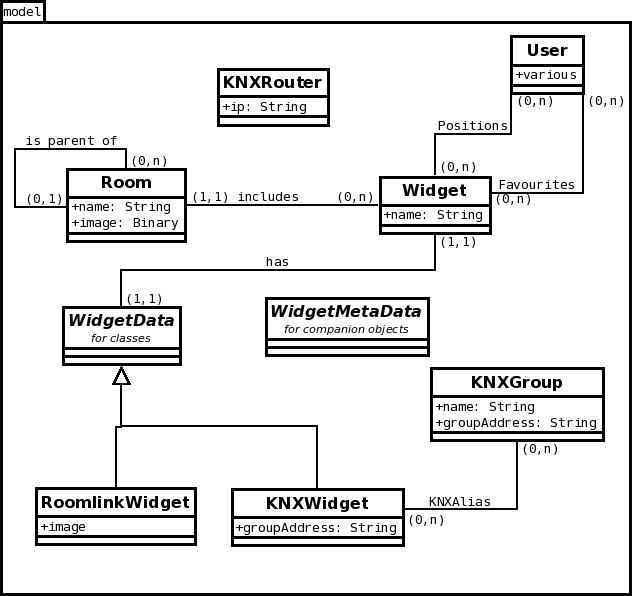
\includegraphics[width=0.80\linewidth]{model.png}
  %% Graphic for TeX using PGF
% Title: /home/alex/Documents/Schule/Diplomarbeit/diplatex/dia/model.dia
% Creator: Dia v0.97
% CreationDate: Mon May 17 13:13:05 2010
% For: alex
% \usepackage{tikz}
% The following commands are not supported in PSTricks at present
% We define them conditionally, so when they are implemented,
% this pgf file will use them.
\ifx\du\undefined
  \newlength{\du}
\fi
\setlength{\du}{15\unitlength}
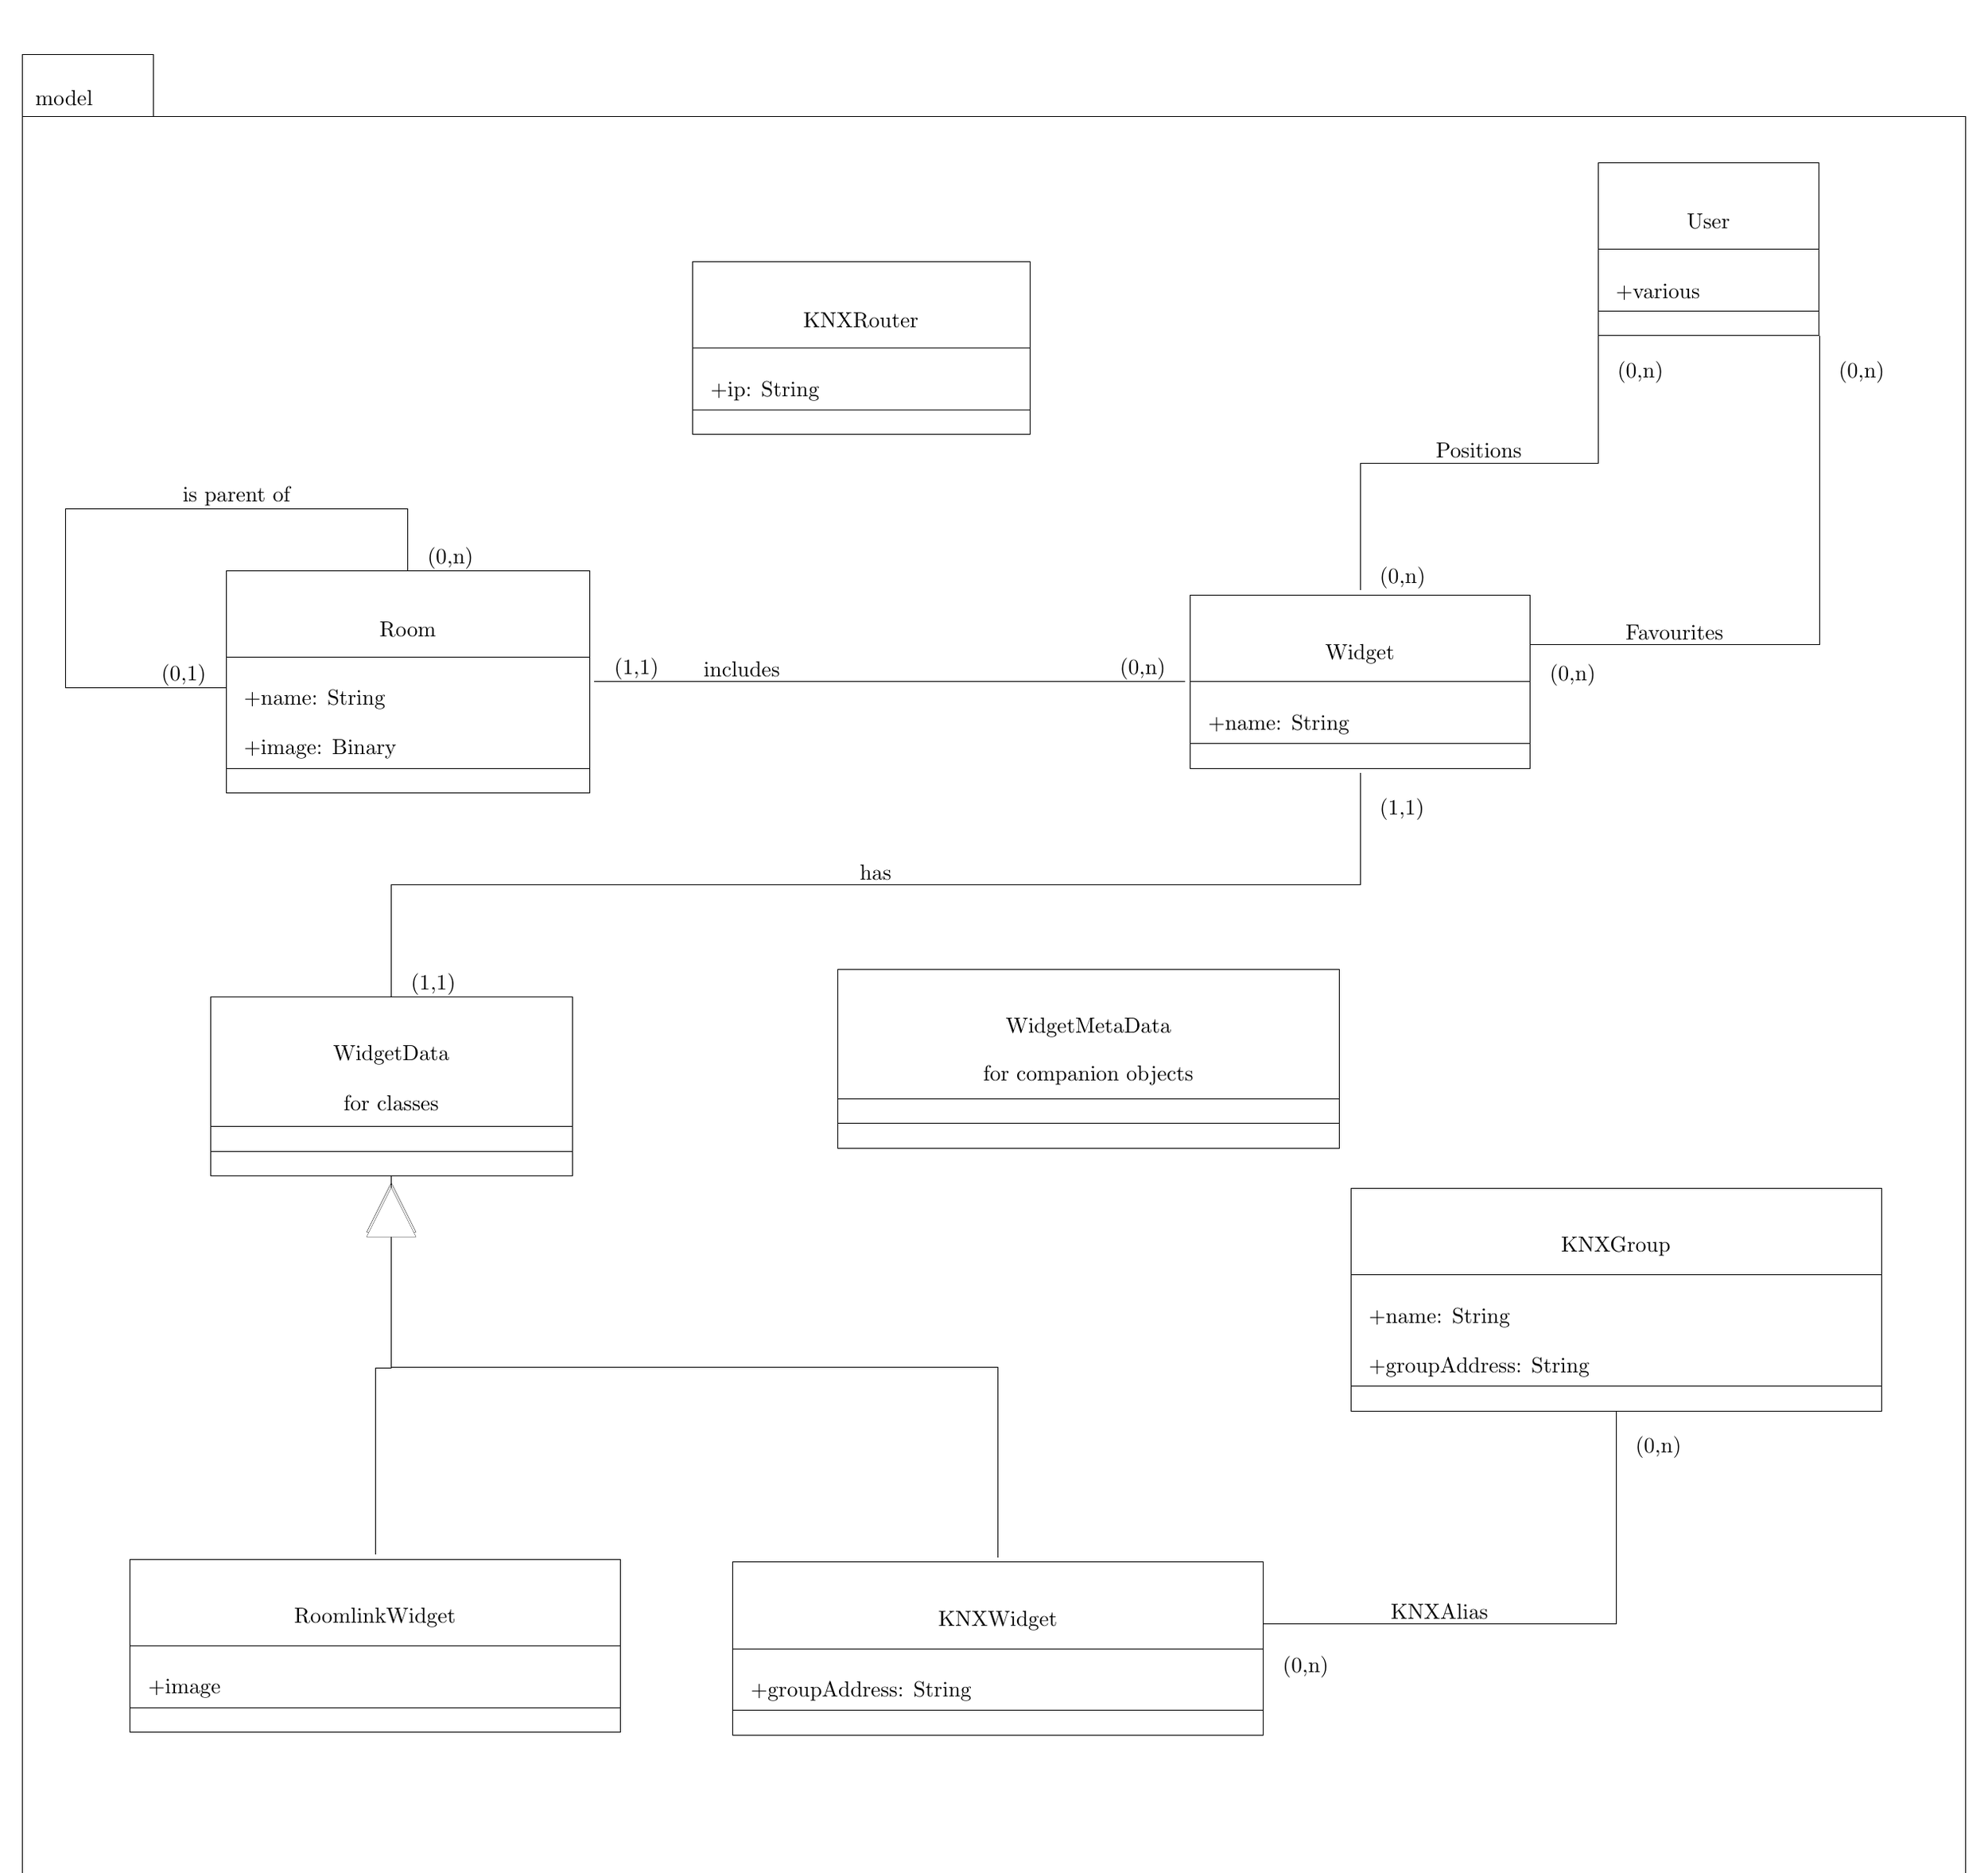
\begin{tikzpicture}
\pgftransformxscale{1.000000}
\pgftransformyscale{-1.000000}
\definecolor{dialinecolor}{rgb}{0.000000, 0.000000, 0.000000}
\pgfsetstrokecolor{dialinecolor}
\definecolor{dialinecolor}{rgb}{1.000000, 1.000000, 1.000000}
\pgfsetfillcolor{dialinecolor}
\pgfsetlinewidth{0.150000\du}
\pgfsetdash{}{0pt}
\definecolor{dialinecolor}{rgb}{1.000000, 1.000000, 1.000000}
\pgfsetfillcolor{dialinecolor}
\fill (15.300000\du,1.300000\du)--(15.300000\du,29.900000\du)--(46.750000\du,29.900000\du)--(46.750000\du,1.300000\du)--cycle;
\definecolor{dialinecolor}{rgb}{0.000000, 0.000000, 0.000000}
\pgfsetstrokecolor{dialinecolor}
\draw (15.300000\du,1.300000\du)--(15.300000\du,29.900000\du)--(46.750000\du,29.900000\du)--(46.750000\du,1.300000\du)--cycle;
\definecolor{dialinecolor}{rgb}{1.000000, 1.000000, 1.000000}
\pgfsetfillcolor{dialinecolor}
\fill (15.300000\du,0.300000\du)--(15.300000\du,1.300000\du)--(17.425000\du,1.300000\du)--(17.425000\du,0.300000\du)--cycle;
\definecolor{dialinecolor}{rgb}{0.000000, 0.000000, 0.000000}
\pgfsetstrokecolor{dialinecolor}
\draw (15.300000\du,0.300000\du)--(15.300000\du,1.300000\du)--(17.425000\du,1.300000\du)--(17.425000\du,0.300000\du)--cycle;
% setfont left to latex
\definecolor{dialinecolor}{rgb}{0.000000, 0.000000, 0.000000}
\pgfsetstrokecolor{dialinecolor}
\node[anchor=west] at (15.400000\du,1.000000\du){model};
\pgfsetlinewidth{0.150000\du}
\pgfsetdash{}{0pt}
\definecolor{dialinecolor}{rgb}{1.000000, 1.000000, 1.000000}
\pgfsetfillcolor{dialinecolor}
\fill (18.600000\du,8.650000\du)--(18.600000\du,10.050000\du)--(24.490000\du,10.050000\du)--(24.490000\du,8.650000\du)--cycle;
\definecolor{dialinecolor}{rgb}{0.000000, 0.000000, 0.000000}
\pgfsetstrokecolor{dialinecolor}
\draw (18.600000\du,8.650000\du)--(18.600000\du,10.050000\du)--(24.490000\du,10.050000\du)--(24.490000\du,8.650000\du)--cycle;
% setfont left to latex
\definecolor{dialinecolor}{rgb}{0.000000, 0.000000, 0.000000}
\pgfsetstrokecolor{dialinecolor}
\node at (21.545000\du,9.600000\du){Room};
\definecolor{dialinecolor}{rgb}{1.000000, 1.000000, 1.000000}
\pgfsetfillcolor{dialinecolor}
\fill (18.600000\du,10.050000\du)--(18.600000\du,11.850000\du)--(24.490000\du,11.850000\du)--(24.490000\du,10.050000\du)--cycle;
\definecolor{dialinecolor}{rgb}{0.000000, 0.000000, 0.000000}
\pgfsetstrokecolor{dialinecolor}
\draw (18.600000\du,10.050000\du)--(18.600000\du,11.850000\du)--(24.490000\du,11.850000\du)--(24.490000\du,10.050000\du)--cycle;
% setfont left to latex
\definecolor{dialinecolor}{rgb}{0.000000, 0.000000, 0.000000}
\pgfsetstrokecolor{dialinecolor}
\node[anchor=west] at (18.775000\du,10.750000\du){+name: String};
% setfont left to latex
\definecolor{dialinecolor}{rgb}{0.000000, 0.000000, 0.000000}
\pgfsetstrokecolor{dialinecolor}
\node[anchor=west] at (18.775000\du,11.550000\du){+image: Binary};
\definecolor{dialinecolor}{rgb}{1.000000, 1.000000, 1.000000}
\pgfsetfillcolor{dialinecolor}
\fill (18.600000\du,11.850000\du)--(18.600000\du,12.250000\du)--(24.490000\du,12.250000\du)--(24.490000\du,11.850000\du)--cycle;
\definecolor{dialinecolor}{rgb}{0.000000, 0.000000, 0.000000}
\pgfsetstrokecolor{dialinecolor}
\draw (18.600000\du,11.850000\du)--(18.600000\du,12.250000\du)--(24.490000\du,12.250000\du)--(24.490000\du,11.850000\du)--cycle;
\pgfsetlinewidth{0.150000\du}
\pgfsetdash{}{0pt}
\definecolor{dialinecolor}{rgb}{1.000000, 1.000000, 1.000000}
\pgfsetfillcolor{dialinecolor}
\fill (34.200000\du,9.050000\du)--(34.200000\du,10.450000\du)--(39.705000\du,10.450000\du)--(39.705000\du,9.050000\du)--cycle;
\definecolor{dialinecolor}{rgb}{0.000000, 0.000000, 0.000000}
\pgfsetstrokecolor{dialinecolor}
\draw (34.200000\du,9.050000\du)--(34.200000\du,10.450000\du)--(39.705000\du,10.450000\du)--(39.705000\du,9.050000\du)--cycle;
% setfont left to latex
\definecolor{dialinecolor}{rgb}{0.000000, 0.000000, 0.000000}
\pgfsetstrokecolor{dialinecolor}
\node at (36.952500\du,10.000000\du){Widget};
\definecolor{dialinecolor}{rgb}{1.000000, 1.000000, 1.000000}
\pgfsetfillcolor{dialinecolor}
\fill (34.200000\du,10.450000\du)--(34.200000\du,11.450000\du)--(39.705000\du,11.450000\du)--(39.705000\du,10.450000\du)--cycle;
\definecolor{dialinecolor}{rgb}{0.000000, 0.000000, 0.000000}
\pgfsetstrokecolor{dialinecolor}
\draw (34.200000\du,10.450000\du)--(34.200000\du,11.450000\du)--(39.705000\du,11.450000\du)--(39.705000\du,10.450000\du)--cycle;
% setfont left to latex
\definecolor{dialinecolor}{rgb}{0.000000, 0.000000, 0.000000}
\pgfsetstrokecolor{dialinecolor}
\node[anchor=west] at (34.375000\du,11.150000\du){+name: String};
\definecolor{dialinecolor}{rgb}{1.000000, 1.000000, 1.000000}
\pgfsetfillcolor{dialinecolor}
\fill (34.200000\du,11.450000\du)--(34.200000\du,11.850000\du)--(39.705000\du,11.850000\du)--(39.705000\du,11.450000\du)--cycle;
\definecolor{dialinecolor}{rgb}{0.000000, 0.000000, 0.000000}
\pgfsetstrokecolor{dialinecolor}
\draw (34.200000\du,11.450000\du)--(34.200000\du,11.850000\du)--(39.705000\du,11.850000\du)--(39.705000\du,11.450000\du)--cycle;
\pgfsetlinewidth{0.150000\du}
\pgfsetdash{}{0pt}
\definecolor{dialinecolor}{rgb}{1.000000, 1.000000, 1.000000}
\pgfsetfillcolor{dialinecolor}
\fill (18.350000\du,15.550000\du)--(18.350000\du,17.650000\du)--(24.205000\du,17.650000\du)--(24.205000\du,15.550000\du)--cycle;
\definecolor{dialinecolor}{rgb}{0.000000, 0.000000, 0.000000}
\pgfsetstrokecolor{dialinecolor}
\draw (18.350000\du,15.550000\du)--(18.350000\du,17.650000\du)--(24.205000\du,17.650000\du)--(24.205000\du,15.550000\du)--cycle;
% setfont left to latex
\definecolor{dialinecolor}{rgb}{0.000000, 0.000000, 0.000000}
\pgfsetstrokecolor{dialinecolor}
\node at (21.277500\du,16.500000\du){WidgetData};
% setfont left to latex
\definecolor{dialinecolor}{rgb}{0.000000, 0.000000, 0.000000}
\pgfsetstrokecolor{dialinecolor}
\node at (21.277500\du,17.275000\du){for classes};
\definecolor{dialinecolor}{rgb}{1.000000, 1.000000, 1.000000}
\pgfsetfillcolor{dialinecolor}
\fill (18.350000\du,17.650000\du)--(18.350000\du,18.050000\du)--(24.205000\du,18.050000\du)--(24.205000\du,17.650000\du)--cycle;
\definecolor{dialinecolor}{rgb}{0.000000, 0.000000, 0.000000}
\pgfsetstrokecolor{dialinecolor}
\draw (18.350000\du,17.650000\du)--(18.350000\du,18.050000\du)--(24.205000\du,18.050000\du)--(24.205000\du,17.650000\du)--cycle;
\definecolor{dialinecolor}{rgb}{1.000000, 1.000000, 1.000000}
\pgfsetfillcolor{dialinecolor}
\fill (18.350000\du,18.050000\du)--(18.350000\du,18.450000\du)--(24.205000\du,18.450000\du)--(24.205000\du,18.050000\du)--cycle;
\definecolor{dialinecolor}{rgb}{0.000000, 0.000000, 0.000000}
\pgfsetstrokecolor{dialinecolor}
\draw (18.350000\du,18.050000\du)--(18.350000\du,18.450000\du)--(24.205000\du,18.450000\du)--(24.205000\du,18.050000\du)--cycle;
\pgfsetlinewidth{0.150000\du}
\pgfsetdash{}{0pt}
\definecolor{dialinecolor}{rgb}{1.000000, 1.000000, 1.000000}
\pgfsetfillcolor{dialinecolor}
\fill (28.500000\du,15.100000\du)--(28.500000\du,17.200000\du)--(36.615000\du,17.200000\du)--(36.615000\du,15.100000\du)--cycle;
\definecolor{dialinecolor}{rgb}{0.000000, 0.000000, 0.000000}
\pgfsetstrokecolor{dialinecolor}
\draw (28.500000\du,15.100000\du)--(28.500000\du,17.200000\du)--(36.615000\du,17.200000\du)--(36.615000\du,15.100000\du)--cycle;
% setfont left to latex
\definecolor{dialinecolor}{rgb}{0.000000, 0.000000, 0.000000}
\pgfsetstrokecolor{dialinecolor}
\node at (32.557500\du,16.050000\du){WidgetMetaData};
% setfont left to latex
\definecolor{dialinecolor}{rgb}{0.000000, 0.000000, 0.000000}
\pgfsetstrokecolor{dialinecolor}
\node at (32.557500\du,16.825000\du){for companion objects};
\definecolor{dialinecolor}{rgb}{1.000000, 1.000000, 1.000000}
\pgfsetfillcolor{dialinecolor}
\fill (28.500000\du,17.200000\du)--(28.500000\du,17.600000\du)--(36.615000\du,17.600000\du)--(36.615000\du,17.200000\du)--cycle;
\definecolor{dialinecolor}{rgb}{0.000000, 0.000000, 0.000000}
\pgfsetstrokecolor{dialinecolor}
\draw (28.500000\du,17.200000\du)--(28.500000\du,17.600000\du)--(36.615000\du,17.600000\du)--(36.615000\du,17.200000\du)--cycle;
\definecolor{dialinecolor}{rgb}{1.000000, 1.000000, 1.000000}
\pgfsetfillcolor{dialinecolor}
\fill (28.500000\du,17.600000\du)--(28.500000\du,18.000000\du)--(36.615000\du,18.000000\du)--(36.615000\du,17.600000\du)--cycle;
\definecolor{dialinecolor}{rgb}{0.000000, 0.000000, 0.000000}
\pgfsetstrokecolor{dialinecolor}
\draw (28.500000\du,17.600000\du)--(28.500000\du,18.000000\du)--(36.615000\du,18.000000\du)--(36.615000\du,17.600000\du)--cycle;
\pgfsetlinewidth{0.100000\du}
\pgfsetdash{}{0pt}
\pgfsetmiterjoin
\pgfsetbuttcap
{
\definecolor{dialinecolor}{rgb}{0.000000, 0.000000, 0.000000}
\pgfsetfillcolor{dialinecolor}
% was here!!!
\definecolor{dialinecolor}{rgb}{0.000000, 0.000000, 0.000000}
\pgfsetstrokecolor{dialinecolor}
\draw (34.127087\du,10.450000\du)--(26.950000\du,10.450000\du)--(26.950000\du,10.450000\du)--(24.564859\du,10.450000\du);
}
% setfont left to latex
\definecolor{dialinecolor}{rgb}{0.000000, 0.000000, 0.000000}
\pgfsetstrokecolor{dialinecolor}
\node at (26.950000\du,10.250000\du){includes};
\definecolor{dialinecolor}{rgb}{0.000000, 0.000000, 0.000000}
\pgfsetstrokecolor{dialinecolor}
\node[anchor=east] at (33.927087\du,10.250000\du){(0,n)};
\definecolor{dialinecolor}{rgb}{0.000000, 0.000000, 0.000000}
\pgfsetstrokecolor{dialinecolor}
\node[anchor=west] at (24.764859\du,10.250000\du){(1,1)};
\pgfsetlinewidth{0.100000\du}
\pgfsetdash{}{0pt}
\pgfsetmiterjoin
\pgfsetbuttcap
{
\definecolor{dialinecolor}{rgb}{0.000000, 0.000000, 0.000000}
\pgfsetfillcolor{dialinecolor}
% was here!!!
\definecolor{dialinecolor}{rgb}{0.000000, 0.000000, 0.000000}
\pgfsetstrokecolor{dialinecolor}
\draw (21.277500\du,15.550000\du)--(21.277500\du,13.737680\du)--(36.952500\du,13.737680\du)--(36.952500\du,11.925360\du);
}
% setfont left to latex
\definecolor{dialinecolor}{rgb}{0.000000, 0.000000, 0.000000}
\pgfsetstrokecolor{dialinecolor}
\node at (29.115000\du,13.537680\du){has};
\definecolor{dialinecolor}{rgb}{0.000000, 0.000000, 0.000000}
\pgfsetstrokecolor{dialinecolor}
\node[anchor=west] at (21.477500\du,15.350000\du){(1,1)};
\definecolor{dialinecolor}{rgb}{0.000000, 0.000000, 0.000000}
\pgfsetstrokecolor{dialinecolor}
\node[anchor=west] at (37.152500\du,12.525360\du){(1,1)};
\pgfsetlinewidth{0.150000\du}
\pgfsetdash{}{0pt}
\definecolor{dialinecolor}{rgb}{1.000000, 1.000000, 1.000000}
\pgfsetfillcolor{dialinecolor}
\fill (26.800000\du,24.700000\du)--(26.800000\du,26.100000\du)--(35.385000\du,26.100000\du)--(35.385000\du,24.700000\du)--cycle;
\definecolor{dialinecolor}{rgb}{0.000000, 0.000000, 0.000000}
\pgfsetstrokecolor{dialinecolor}
\draw (26.800000\du,24.700000\du)--(26.800000\du,26.100000\du)--(35.385000\du,26.100000\du)--(35.385000\du,24.700000\du)--cycle;
% setfont left to latex
\definecolor{dialinecolor}{rgb}{0.000000, 0.000000, 0.000000}
\pgfsetstrokecolor{dialinecolor}
\node at (31.092500\du,25.650000\du){KNXWidget};
\definecolor{dialinecolor}{rgb}{1.000000, 1.000000, 1.000000}
\pgfsetfillcolor{dialinecolor}
\fill (26.800000\du,26.100000\du)--(26.800000\du,27.100000\du)--(35.385000\du,27.100000\du)--(35.385000\du,26.100000\du)--cycle;
\definecolor{dialinecolor}{rgb}{0.000000, 0.000000, 0.000000}
\pgfsetstrokecolor{dialinecolor}
\draw (26.800000\du,26.100000\du)--(26.800000\du,27.100000\du)--(35.385000\du,27.100000\du)--(35.385000\du,26.100000\du)--cycle;
% setfont left to latex
\definecolor{dialinecolor}{rgb}{0.000000, 0.000000, 0.000000}
\pgfsetstrokecolor{dialinecolor}
\node[anchor=west] at (26.975000\du,26.800000\du){+groupAddress: String};
\definecolor{dialinecolor}{rgb}{1.000000, 1.000000, 1.000000}
\pgfsetfillcolor{dialinecolor}
\fill (26.800000\du,27.100000\du)--(26.800000\du,27.500000\du)--(35.385000\du,27.500000\du)--(35.385000\du,27.100000\du)--cycle;
\definecolor{dialinecolor}{rgb}{0.000000, 0.000000, 0.000000}
\pgfsetstrokecolor{dialinecolor}
\draw (26.800000\du,27.100000\du)--(26.800000\du,27.500000\du)--(35.385000\du,27.500000\du)--(35.385000\du,27.100000\du)--cycle;
\pgfsetlinewidth{0.150000\du}
\pgfsetdash{}{0pt}
\definecolor{dialinecolor}{rgb}{1.000000, 1.000000, 1.000000}
\pgfsetfillcolor{dialinecolor}
\fill (17.050000\du,24.650000\du)--(17.050000\du,26.050000\du)--(24.977500\du,26.050000\du)--(24.977500\du,24.650000\du)--cycle;
\definecolor{dialinecolor}{rgb}{0.000000, 0.000000, 0.000000}
\pgfsetstrokecolor{dialinecolor}
\draw (17.050000\du,24.650000\du)--(17.050000\du,26.050000\du)--(24.977500\du,26.050000\du)--(24.977500\du,24.650000\du)--cycle;
% setfont left to latex
\definecolor{dialinecolor}{rgb}{0.000000, 0.000000, 0.000000}
\pgfsetstrokecolor{dialinecolor}
\node at (21.013750\du,25.600000\du){RoomlinkWidget};
\definecolor{dialinecolor}{rgb}{1.000000, 1.000000, 1.000000}
\pgfsetfillcolor{dialinecolor}
\fill (17.050000\du,26.050000\du)--(17.050000\du,27.050000\du)--(24.977500\du,27.050000\du)--(24.977500\du,26.050000\du)--cycle;
\definecolor{dialinecolor}{rgb}{0.000000, 0.000000, 0.000000}
\pgfsetstrokecolor{dialinecolor}
\draw (17.050000\du,26.050000\du)--(17.050000\du,27.050000\du)--(24.977500\du,27.050000\du)--(24.977500\du,26.050000\du)--cycle;
% setfont left to latex
\definecolor{dialinecolor}{rgb}{0.000000, 0.000000, 0.000000}
\pgfsetstrokecolor{dialinecolor}
\node[anchor=west] at (17.225000\du,26.750000\du){+image};
\definecolor{dialinecolor}{rgb}{1.000000, 1.000000, 1.000000}
\pgfsetfillcolor{dialinecolor}
\fill (17.050000\du,27.050000\du)--(17.050000\du,27.450000\du)--(24.977500\du,27.450000\du)--(24.977500\du,27.050000\du)--cycle;
\definecolor{dialinecolor}{rgb}{0.000000, 0.000000, 0.000000}
\pgfsetstrokecolor{dialinecolor}
\draw (17.050000\du,27.050000\du)--(17.050000\du,27.450000\du)--(24.977500\du,27.450000\du)--(24.977500\du,27.050000\du)--cycle;
\pgfsetlinewidth{0.100000\du}
\pgfsetdash{}{0pt}
\pgfsetmiterjoin
\pgfsetbuttcap
{
\definecolor{dialinecolor}{rgb}{0.000000, 0.000000, 0.000000}
\pgfsetfillcolor{dialinecolor}
% was here!!!
\definecolor{dialinecolor}{rgb}{0.000000, 0.000000, 0.000000}
\pgfsetstrokecolor{dialinecolor}
\draw (21.277500\du,18.450000\du)--(21.277500\du,21.537320\du)--(31.092500\du,21.537320\du)--(31.092500\du,24.624640\du);
}
\definecolor{dialinecolor}{rgb}{0.000000, 0.000000, 0.000000}
\pgfsetstrokecolor{dialinecolor}
\draw (21.277500\du,19.361803\du)--(21.277500\du,21.537320\du)--(31.092500\du,21.537320\du)--(31.092500\du,24.624640\du);
\pgfsetmiterjoin
\definecolor{dialinecolor}{rgb}{1.000000, 1.000000, 1.000000}
\pgfsetfillcolor{dialinecolor}
\fill (21.677500\du,19.361803\du)--(21.277500\du,18.561803\du)--(20.877500\du,19.361803\du)--cycle;
\pgfsetlinewidth{0.100000\du}
\pgfsetdash{}{0pt}
\pgfsetmiterjoin
\definecolor{dialinecolor}{rgb}{0.000000, 0.000000, 0.000000}
\pgfsetstrokecolor{dialinecolor}
\draw (21.677500\du,19.361803\du)--(21.277500\du,18.561803\du)--(20.877500\du,19.361803\du)--cycle;
% setfont left to latex
\pgfsetlinewidth{0.100000\du}
\pgfsetdash{}{0pt}
\pgfsetmiterjoin
\pgfsetbuttcap
{
\definecolor{dialinecolor}{rgb}{0.000000, 0.000000, 0.000000}
\pgfsetfillcolor{dialinecolor}
% was here!!!
\definecolor{dialinecolor}{rgb}{0.000000, 0.000000, 0.000000}
\pgfsetstrokecolor{dialinecolor}
\draw (21.277500\du,18.525372\du)--(21.277500\du,21.550006\du)--(21.013750\du,21.550006\du)--(21.013750\du,24.574640\du);
}
\definecolor{dialinecolor}{rgb}{0.000000, 0.000000, 0.000000}
\pgfsetstrokecolor{dialinecolor}
\draw (21.277500\du,19.437176\du)--(21.277500\du,21.550006\du)--(21.013750\du,21.550006\du)--(21.013750\du,24.574640\du);
\pgfsetmiterjoin
\definecolor{dialinecolor}{rgb}{1.000000, 1.000000, 1.000000}
\pgfsetfillcolor{dialinecolor}
\fill (21.677500\du,19.437176\du)--(21.277500\du,18.637176\du)--(20.877500\du,19.437176\du)--cycle;
\pgfsetlinewidth{0.100000\du}
\pgfsetdash{}{0pt}
\pgfsetmiterjoin
\definecolor{dialinecolor}{rgb}{0.000000, 0.000000, 0.000000}
\pgfsetstrokecolor{dialinecolor}
\draw (21.677500\du,19.437176\du)--(21.277500\du,18.637176\du)--(20.877500\du,19.437176\du)--cycle;
% setfont left to latex
\pgfsetlinewidth{0.150000\du}
\pgfsetdash{}{0pt}
\definecolor{dialinecolor}{rgb}{1.000000, 1.000000, 1.000000}
\pgfsetfillcolor{dialinecolor}
\fill (40.800000\du,2.050000\du)--(40.800000\du,3.450000\du)--(44.380000\du,3.450000\du)--(44.380000\du,2.050000\du)--cycle;
\definecolor{dialinecolor}{rgb}{0.000000, 0.000000, 0.000000}
\pgfsetstrokecolor{dialinecolor}
\draw (40.800000\du,2.050000\du)--(40.800000\du,3.450000\du)--(44.380000\du,3.450000\du)--(44.380000\du,2.050000\du)--cycle;
% setfont left to latex
\definecolor{dialinecolor}{rgb}{0.000000, 0.000000, 0.000000}
\pgfsetstrokecolor{dialinecolor}
\node at (42.590000\du,3.000000\du){User};
\definecolor{dialinecolor}{rgb}{1.000000, 1.000000, 1.000000}
\pgfsetfillcolor{dialinecolor}
\fill (40.800000\du,3.450000\du)--(40.800000\du,4.450000\du)--(44.380000\du,4.450000\du)--(44.380000\du,3.450000\du)--cycle;
\definecolor{dialinecolor}{rgb}{0.000000, 0.000000, 0.000000}
\pgfsetstrokecolor{dialinecolor}
\draw (40.800000\du,3.450000\du)--(40.800000\du,4.450000\du)--(44.380000\du,4.450000\du)--(44.380000\du,3.450000\du)--cycle;
% setfont left to latex
\definecolor{dialinecolor}{rgb}{0.000000, 0.000000, 0.000000}
\pgfsetstrokecolor{dialinecolor}
\node[anchor=west] at (40.975000\du,4.150000\du){+various};
\definecolor{dialinecolor}{rgb}{1.000000, 1.000000, 1.000000}
\pgfsetfillcolor{dialinecolor}
\fill (40.800000\du,4.450000\du)--(40.800000\du,4.850000\du)--(44.380000\du,4.850000\du)--(44.380000\du,4.450000\du)--cycle;
\definecolor{dialinecolor}{rgb}{0.000000, 0.000000, 0.000000}
\pgfsetstrokecolor{dialinecolor}
\draw (40.800000\du,4.450000\du)--(40.800000\du,4.850000\du)--(44.380000\du,4.850000\du)--(44.380000\du,4.450000\du)--cycle;
\pgfsetlinewidth{0.100000\du}
\pgfsetdash{}{0pt}
\pgfsetmiterjoin
\pgfsetbuttcap
{
\definecolor{dialinecolor}{rgb}{0.000000, 0.000000, 0.000000}
\pgfsetfillcolor{dialinecolor}
% was here!!!
\definecolor{dialinecolor}{rgb}{0.000000, 0.000000, 0.000000}
\pgfsetstrokecolor{dialinecolor}
\draw (36.952500\du,8.974640\du)--(36.952500\du,6.912320\du)--(40.800000\du,6.912320\du)--(40.800000\du,4.850000\du);
}
% setfont left to latex
\definecolor{dialinecolor}{rgb}{0.000000, 0.000000, 0.000000}
\pgfsetstrokecolor{dialinecolor}
\node at (38.876250\du,6.712320\du){Positions};
\definecolor{dialinecolor}{rgb}{0.000000, 0.000000, 0.000000}
\pgfsetstrokecolor{dialinecolor}
\node[anchor=west] at (37.152500\du,8.774640\du){(0,n)};
\definecolor{dialinecolor}{rgb}{0.000000, 0.000000, 0.000000}
\pgfsetstrokecolor{dialinecolor}
\node[anchor=west] at (41.000000\du,5.450000\du){(0,n)};
\pgfsetlinewidth{0.150000\du}
\pgfsetdash{}{0pt}
\definecolor{dialinecolor}{rgb}{1.000000, 1.000000, 1.000000}
\pgfsetfillcolor{dialinecolor}
\fill (36.800000\du,18.650000\du)--(36.800000\du,20.050000\du)--(45.385000\du,20.050000\du)--(45.385000\du,18.650000\du)--cycle;
\definecolor{dialinecolor}{rgb}{0.000000, 0.000000, 0.000000}
\pgfsetstrokecolor{dialinecolor}
\draw (36.800000\du,18.650000\du)--(36.800000\du,20.050000\du)--(45.385000\du,20.050000\du)--(45.385000\du,18.650000\du)--cycle;
% setfont left to latex
\definecolor{dialinecolor}{rgb}{0.000000, 0.000000, 0.000000}
\pgfsetstrokecolor{dialinecolor}
\node at (41.092500\du,19.600000\du){KNXGroup};
\definecolor{dialinecolor}{rgb}{1.000000, 1.000000, 1.000000}
\pgfsetfillcolor{dialinecolor}
\fill (36.800000\du,20.050000\du)--(36.800000\du,21.850000\du)--(45.385000\du,21.850000\du)--(45.385000\du,20.050000\du)--cycle;
\definecolor{dialinecolor}{rgb}{0.000000, 0.000000, 0.000000}
\pgfsetstrokecolor{dialinecolor}
\draw (36.800000\du,20.050000\du)--(36.800000\du,21.850000\du)--(45.385000\du,21.850000\du)--(45.385000\du,20.050000\du)--cycle;
% setfont left to latex
\definecolor{dialinecolor}{rgb}{0.000000, 0.000000, 0.000000}
\pgfsetstrokecolor{dialinecolor}
\node[anchor=west] at (36.975000\du,20.750000\du){+name: String};
% setfont left to latex
\definecolor{dialinecolor}{rgb}{0.000000, 0.000000, 0.000000}
\pgfsetstrokecolor{dialinecolor}
\node[anchor=west] at (36.975000\du,21.550000\du){+groupAddress: String};
\definecolor{dialinecolor}{rgb}{1.000000, 1.000000, 1.000000}
\pgfsetfillcolor{dialinecolor}
\fill (36.800000\du,21.850000\du)--(36.800000\du,22.250000\du)--(45.385000\du,22.250000\du)--(45.385000\du,21.850000\du)--cycle;
\definecolor{dialinecolor}{rgb}{0.000000, 0.000000, 0.000000}
\pgfsetstrokecolor{dialinecolor}
\draw (36.800000\du,21.850000\du)--(36.800000\du,22.250000\du)--(45.385000\du,22.250000\du)--(45.385000\du,21.850000\du)--cycle;
\pgfsetlinewidth{0.100000\du}
\pgfsetdash{}{0pt}
\pgfsetmiterjoin
\pgfsetbuttcap
{
\definecolor{dialinecolor}{rgb}{0.000000, 0.000000, 0.000000}
\pgfsetfillcolor{dialinecolor}
% was here!!!
\definecolor{dialinecolor}{rgb}{0.000000, 0.000000, 0.000000}
\pgfsetstrokecolor{dialinecolor}
\draw (41.092500\du,22.250000\du)--(41.092500\du,25.700000\du)--(35.385000\du,25.700000\du)--(35.385000\du,26.600000\du);
}
% setfont left to latex
\definecolor{dialinecolor}{rgb}{0.000000, 0.000000, 0.000000}
\pgfsetstrokecolor{dialinecolor}
\node at (38.238750\du,25.500000\du){KNXAlias};
\definecolor{dialinecolor}{rgb}{0.000000, 0.000000, 0.000000}
\pgfsetstrokecolor{dialinecolor}
\node[anchor=west] at (41.292500\du,22.850000\du){(0,n)};
\definecolor{dialinecolor}{rgb}{0.000000, 0.000000, 0.000000}
\pgfsetstrokecolor{dialinecolor}
\node[anchor=west] at (35.585000\du,26.400000\du){(0,n)};
\pgfsetlinewidth{0.150000\du}
\pgfsetdash{}{0pt}
\definecolor{dialinecolor}{rgb}{1.000000, 1.000000, 1.000000}
\pgfsetfillcolor{dialinecolor}
\fill (26.150000\du,3.650000\du)--(26.150000\du,5.050000\du)--(31.605000\du,5.050000\du)--(31.605000\du,3.650000\du)--cycle;
\definecolor{dialinecolor}{rgb}{0.000000, 0.000000, 0.000000}
\pgfsetstrokecolor{dialinecolor}
\draw (26.150000\du,3.650000\du)--(26.150000\du,5.050000\du)--(31.605000\du,5.050000\du)--(31.605000\du,3.650000\du)--cycle;
% setfont left to latex
\definecolor{dialinecolor}{rgb}{0.000000, 0.000000, 0.000000}
\pgfsetstrokecolor{dialinecolor}
\node at (28.877500\du,4.600000\du){KNXRouter};
\definecolor{dialinecolor}{rgb}{1.000000, 1.000000, 1.000000}
\pgfsetfillcolor{dialinecolor}
\fill (26.150000\du,5.050000\du)--(26.150000\du,6.050000\du)--(31.605000\du,6.050000\du)--(31.605000\du,5.050000\du)--cycle;
\definecolor{dialinecolor}{rgb}{0.000000, 0.000000, 0.000000}
\pgfsetstrokecolor{dialinecolor}
\draw (26.150000\du,5.050000\du)--(26.150000\du,6.050000\du)--(31.605000\du,6.050000\du)--(31.605000\du,5.050000\du)--cycle;
% setfont left to latex
\definecolor{dialinecolor}{rgb}{0.000000, 0.000000, 0.000000}
\pgfsetstrokecolor{dialinecolor}
\node[anchor=west] at (26.325000\du,5.750000\du){+ip: String};
\definecolor{dialinecolor}{rgb}{1.000000, 1.000000, 1.000000}
\pgfsetfillcolor{dialinecolor}
\fill (26.150000\du,6.050000\du)--(26.150000\du,6.450000\du)--(31.605000\du,6.450000\du)--(31.605000\du,6.050000\du)--cycle;
\definecolor{dialinecolor}{rgb}{0.000000, 0.000000, 0.000000}
\pgfsetstrokecolor{dialinecolor}
\draw (26.150000\du,6.050000\du)--(26.150000\du,6.450000\du)--(31.605000\du,6.450000\du)--(31.605000\du,6.050000\du)--cycle;
\pgfsetlinewidth{0.100000\du}
\pgfsetdash{}{0pt}
\pgfsetmiterjoin
\pgfsetbuttcap
{
\definecolor{dialinecolor}{rgb}{0.000000, 0.000000, 0.000000}
\pgfsetfillcolor{dialinecolor}
% was here!!!
\definecolor{dialinecolor}{rgb}{0.000000, 0.000000, 0.000000}
\pgfsetstrokecolor{dialinecolor}
\draw (39.705000\du,9.750000\du)--(39.705000\du,9.850000\du)--(44.380000\du,9.850000\du)--(44.380000\du,4.850000\du);
}
% setfont left to latex
\definecolor{dialinecolor}{rgb}{0.000000, 0.000000, 0.000000}
\pgfsetstrokecolor{dialinecolor}
\node at (42.042500\du,9.650000\du){Favourites};
\definecolor{dialinecolor}{rgb}{0.000000, 0.000000, 0.000000}
\pgfsetstrokecolor{dialinecolor}
\node[anchor=west] at (39.905000\du,10.350000\du){(0,n)};
\definecolor{dialinecolor}{rgb}{0.000000, 0.000000, 0.000000}
\pgfsetstrokecolor{dialinecolor}
\node[anchor=west] at (44.580000\du,5.450000\du){(0,n)};
\pgfsetlinewidth{0.100000\du}
\pgfsetdash{}{0pt}
\pgfsetmiterjoin
\pgfsetbuttcap
{
\definecolor{dialinecolor}{rgb}{0.000000, 0.000000, 0.000000}
\pgfsetfillcolor{dialinecolor}
% was here!!!
\definecolor{dialinecolor}{rgb}{0.000000, 0.000000, 0.000000}
\pgfsetstrokecolor{dialinecolor}
\draw (18.600000\du,10.550000\du)--(16.000000\du,10.550000\du)--(16.000000\du,7.650000\du)--(21.545000\du,7.650000\du)--(21.545000\du,8.650000\du);
}
% setfont left to latex
\definecolor{dialinecolor}{rgb}{0.000000, 0.000000, 0.000000}
\pgfsetstrokecolor{dialinecolor}
\node at (18.772500\du,7.450000\du){is parent of};
\definecolor{dialinecolor}{rgb}{0.000000, 0.000000, 0.000000}
\pgfsetstrokecolor{dialinecolor}
\node[anchor=east] at (18.400000\du,10.350000\du){(0,1)};
\definecolor{dialinecolor}{rgb}{0.000000, 0.000000, 0.000000}
\pgfsetstrokecolor{dialinecolor}
\node[anchor=west] at (21.745000\du,8.450000\du){(0,n)};
\end{tikzpicture}

  \caption{database structure}
  \label{fig:model}
  \end{figure}

The \lstinline!User! table uses Lift's \lstinline!MegaProtoUser! to save user data. This is used to save separate widget positions and favourites per user. The \lstinline!Room! table is used to model the room structure. A room without a parent is considered to be a root room. The \lstinline!Widget! table itself only saves the name of a widget, it is mostly used to provide a single endpoint for all the relations that should lead to the different \lstinline!WidgetData! subclasses. \lstinline!WidgetData! is the trait that needs to be mixed in by all the tables that represent different widget types, their companion objects must mix in \lstinline!WidgetMetaData!. \lstinline!Widget! also has some convenience methods that make it easier to implement new \lstinline!WidgetData! tables. The \lstinline!RoomlinkWidget! and \lstinline!KNXWidget! classes are the \lstinline!WidgetData! implementations for Roomlinks and KNX widgets, respectively. \lstinline!KNXGroup! provides a device to assign multiple KNX addresses to a single KNX widget. Finally, \lstinline!KNXRouter! is a table that contains only a single row, which contains the IP address of the KNX router used to access the local KNX network.

\section{Widget Structure}
To make the widget structure in Sombrero more understandable this diagram was created. It shows the inheritance between the widget Scala classes and it describes the interface between client JavaScript widgets and server Scala classes. All Scala classes are in the placed in Lift box and all JavaScript classes in the JavaScript box.

The JavaScript widgets are all JQuery UI widgets and represent the three types of widgets, which are described in chapter User Mode. These widgets are configurable. This configuration is done by the Scala widget classes. Through this configuration the JQuery UI widgets can be adopted to a special kind of device widget like lamp. It's also possible to use this create a non KNX widget like the room link widget.  

During the rendering process is all JQuery UI widget code provided by the Scala classes and on page load are all initialized. The Scala classes now communicate with the JQuery UI widgets through AJAX and Comet. To ease the interface between JavaScript and Scala the class JavaScriptHelper was build. 
  \begin{figure}[h]
  \centering
  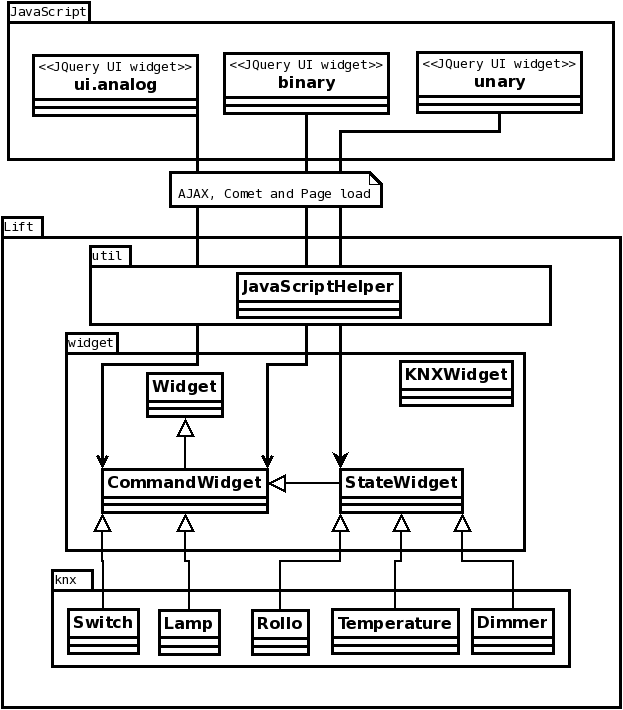
\includegraphics[width=0.80\linewidth]{widgets.png}
  %\input{widgets}
  \caption{widget structure}
  \label{fig:widgets}
  \end{figure}

	\clearpage
\glossary{ name=Individualsoftware, description={Individualsoftware zeichnet sich dadurch aus, dass sie nur f�r einen oder f�r wenige Anwendungsf�lle geschaffen wird.}}
\clearpage
	
	%--------------------------------------------------------------------------
	% Anhang
	%--------------------------------------------------------------------------

	%\chapter[List of Figures]{}

		\addcontentsline{toc}{chapter}{List of Figures}
	\listoffigures
	\clearpage
	
	%\addcontentsline{toc}{section}{List of Tables}
	%\listoftables
	%\clearpage

	\addcontentsline{toc}{chapter}{List of Listings}
	\lstlistoflistings
	\clearpage
	
    	\addcontentsline{toc}{chapter}{Glossary}
    \printglossary 
	\clearpage


  	\addcontentsline{toc}{chapter}{Index}
  \printindex
  \clearpage

	%\bibliographystyle{alpha} 		 %Standardstyle
	%\bibliographystyle{dinat}		 %Style und Layout nach DIN 1502
	%\bibliography{tiger}					 %Literaturverzeichnis einf�gen
	
	\clearpage
	\addcontentsline{toc}{chapter}{Bibliography}
		%So kann zitiert werden (sollte in einer der Unterdateien sein)
	%\citep[vgl. Seite 22]{kopka1:00}
	\begin{thebibliography}{999}
		\bibitem{odersky:08} Martin Odersky, Lex Spoon, Bill Venners:
		  \emph{Programming in Scala},
		  Artima, 2008  \\
		  ISBN: 978-0-9815316-0-1
		\bibitem{pollak:09} David Pollak:
		  \emph{Beginning Scala},
		  Apress, 2009  \\
		  ISBN: 978-1-4302-1989-7
		\bibitem{scala-lang.org}
		  the Scala homepage, \\
		  \url{http://www.scala-lang.org/}
		\bibitem{scala-lang.org:api}
		  the Scala API, \\
		  \url{http://www.scala-lang.org/docu/files/api/index.html}
		\bibitem{scala-lang.org:manuals}
		  official Scala manuals, \\
		  \url{http://www.scala-lang.org/node/198}
		\bibitem{becker:09} Derek Chen-Becker, Tyler Weir, Marius Danciu:
		  \emph{The Definitive Guide to Lift},
		  Apress, 2009  \\
		  ISBN: 978-1-4302-2421-1
		\bibitem{liftweb.net}
		  the Lift homepage, \\
		  \url{http://liftweb.net/}
	  \bibitem{liftweb.net:api}
	    the Lift API, \\
	    \url{http://scala-tools.org/scaladocs/liftweb/1.0/}
	  \bibitem{37signals:10} 37signals, Jason Fried, David Heinemeier Hansson, Matthew Linderman:
	    \emph{Getting Real},
		  37signals, LLC., 2006  \\
		  ISBN: 978-0-578-01281-0
		\bibitem{wilkins:95} David R. Wilkins:
		  \emph{Getting Started with LaTeX} (2nd Edition), 1995 \\
		  \url{http://www.maths.tcd.ie/~dwilkins/LaTeXPrimer/GSWLaTeX.pdf}
		\bibitem{auto.tuwien.ac.at:calimero}
		  Calimero documentation, \\
		  \url{http://www.auto.tuwien.ac.at/downloads/calimero-ng.pdf}
		\bibitem{auto.tuwien.ac.at:knx05}
		  Open-source foundations for PC based KNX/EIB access and management - \\
      Presentation given at the 2005 Konnex Scientific Conference including information on Calimero. \\
		  \url{https://www.auto.tuwien.ac.at/downloads/knxsci05/knx05-access.pdf}
		\bibitem{castledine:10} Earle Castledine, Craig Sharkie:
		  \emph{jQuery: Novice to Ninja},
      SitePoint, 2010 \\
      ISBN: 978-0-9805768-5-6
		\bibitem{htlwrn.ac.at}
		  HTBLuVA Wiener Neustadt homepage, \\
		  \url{http://www.htlwrn.ac.at/}
		\bibitem{auto.tuwien.ac.at:a-lab}
		  A-Lab homepage, \\
		  \url{https://www.auto.tuwien.ac.at/a-lab/home.html}
		\bibitem{fh-degendorf.de:knxathome}
		  KNX@home homepage, \\
		  \url{http://knxathome.fh-deggendorf.de/}
		\bibitem{linuxmce.org}
		  LinuxMCE homepage, \\
		  \url{http://www.linuxmce.org/}
		    \bibitem{google.com:liftgroup}
         Lift User Group, \\
         \url{http://groups.google.com/group/liftweb}
        \bibitem{wikipedia.org:agile}
         Agile software development, \\
         \url{http://en.wikipedia.org/wiki/Agile_software_development}
        \bibitem{agilemanifesto.org}
         Agile Manifesto, \\
         \url{http://agilemanifesto.org/}
        \bibitem{auto.tuwien.ac.at:calimeropdf}
         Calimero NG documentation, \\
         \url{http://www.auto.tuwien.ac.at/downloads/calimero-ng.pdf}
        \bibitem{knx.org}
         What is KNX, \\
         \url{http://www.knx.org/knx/what-is-knx/}
        \bibitem{wikipedia.org:knx}
         A short KNX documentation, \\
         \url{http://en.wikipedia.org/wiki/KNX_(standard}
        \bibitem{wikipedia.org:javascript}
         A short JavaScript documentation, \\
         \url{http://en.wikipedia.org/wiki/Javascript}
        \bibitem{wikipedia.org:ajax}
         A short AJAX documentation, \\
         \url{http://en.wikipedia.org/wiki/Ajax_(programming)}
        \bibitem{wikipedia.org:comet}
         A short Comet documentation, \\
         \url{http://en.wikipedia.org/wiki/Comet_(programming)}
        \bibitem{wikipedia.org:jquery}
         A short JQuery documentation, \\
         \url{http://en.wikipedia.org/wiki/JQuery}
        \bibitem{jqueryui.com}
         JQuery UI homepage, \\
         \url{http://jqueryui.com/}
        \bibitem{bassistance.de}
         JQuery-message plugin homepage, \\
         \url{http://bassistance.de/jquery-plugins/jquery-plugin-message/}
        \bibitem{jquery.com:collision}
         A short documentation of the collision plugin, \\
         \url{http://plugins.jquery.com/taxonomy/term/1837}
        \bibitem{fancybox.net}
         FancyBox homepage, \\
         \url{http://fancybox.net/}
        \bibitem{filamentgroup.com:ipod}
         The homepage of iPod-style drilldown menu, \\
         \url{http://www.filamentgroup.com/lab/jquery_ipod_style_drilldown_menu/}
        \bibitem{wikipedia.org:css}
         A short documentation of CSS, \\
         \url{http://en.wikipedia.org/wiki/Cascading_Style_Sheets}
        \bibitem{yaml.de}
         Yaml homepage, \\
         \url{http://www.yaml.de/}
        \bibitem{apache.org:maven}
         Maven homepage, \\
         \url{maven.apache.org}
        \bibitem{eclipse.org:egit}
         EGit homepage, \\
         \url{http://www.eclipse.org/egit/}
        \bibitem{eclipse.org}
         eclipse homepage, \\
         \url{http://www.eclipse.org/}
	\end{thebibliography}

    \clearpage
\end{document}
